\documentclass{beamer}
\usepackage[latin1]{inputenc}
\usepackage{graphicx}
\usepackage{tipa}
\usepackage{appendixnumberbeamer}

\newcommand\Wider[2][3em]{
\makebox[\linewidth][c]{
  \begin{minipage}{\dimexpr\textwidth+#1\relax}
  \raggedright#2
  \end{minipage}
  }
}

\newcommand{\Bz}{$B_0$}

\usetheme{Madrid}

\title[BnoC Status Report]{BnoC Status Report}
\author[Tim Williams]{Tim Williams on behalf of the BnoC PWG}
\institute[Birmingham]{84th \lhcb week}
\titlegraphic{
\includegraphics[height=2.1cm]{UoBLogo}}%\hspace*{2cm}
\includegraphics[height=2cm]{LhcbLogo}}
\date{13/06/2017}

\usepackage{ifthen} 
\newboolean{uprightparticles}
\setboolean{uprightparticles}{false} %Set true for upright particle symbols
\usepackage{xspace} 
\usepackage{upgreek}

%%% $Id: lhcb-symbols-def.tex 43084 2013-10-29 12:59:55Z roldeman $
%%% ======================================================================
%%% Purpose: Standard LHCb aliases
%%% Author: Originally Ulrik Egede, adapted by Tomasz Skwarnicki for templates,
%%% rewritten by Chris Parkes
%%% Maintainer : Ulrik Egede (2010 - 2012)
%%% =======================================================================

%%% To use this file outside the normal LHCb document environment, the
%%% following should be added in a preamble (before \begin{document}
%%%
%%%\usepackage{ifthen} 
%%%\newboolean{uprightparticles}
%%%\setboolean{uprightparticles}{false} %Set true for upright particle symbols
%%% \usepackage{xspace} 
%%% \usepackage{upgreek}

%%%%%%%%%%%%%%%%%%%%%%%%%%%%%%%%%%%%%%%%%%%%%%%%%%%%%%%%%%%%
%%%
%%% The following is to ensure that the template automatically can process
%%% this file.
%%%
%%% Add comments with at least three %%% preceding.
%%% Add new sections with one % preceding
%%% Add new subsections with two %% preceding
%%%%%%%%%%%%%%%%%%%%%%%%%%%%%%%%%%%%%%%%%%%%%%%%%%%%%%%%%%%%

%%%%%%%%%%%%%
% Experiments
%%%%%%%%%%%%%
\def\lhcb {\mbox{LHCb}\xspace}
\def\atlas  {\mbox{ATLAS}\xspace}
\def\cms    {\mbox{CMS}\xspace}
\def\alice  {\mbox{ALICE}\xspace}
\def\babar  {\mbox{BaBar}\xspace}
\def\belle  {\mbox{Belle}\xspace}
\def\cleo   {\mbox{CLEO}\xspace}
\def\cdf    {\mbox{CDF}\xspace}
\def\dzero  {\mbox{D0}\xspace}
\def\aleph  {\mbox{ALEPH}\xspace}
\def\delphi {\mbox{DELPHI}\xspace}
\def\opal   {\mbox{OPAL}\xspace}
\def\lthree {\mbox{L3}\xspace}
\def\sld    {\mbox{SLD}\xspace}
%%%\def\argus  {\mbox{ARGUS}\xspace}
%%%\def\uaone  {\mbox{UA1}\xspace}
%%%\def\uatwo  {\mbox{UA2}\xspace}
%%%\def\ux85 {\mbox{UX85}\xspace}
\def\cern {\mbox{CERN}\xspace}
\def\lhc    {\mbox{LHC}\xspace}
\def\lep    {\mbox{LEP}\xspace}
\def\tevatron {Tevatron\xspace}

%% LHCb sub-detectors and sub-systems

%%%\def\pu     {PU\xspace}
\def\velo   {VELO\xspace}
\def\rich   {RICH\xspace}
\def\richone {RICH1\xspace}
\def\richtwo {RICH2\xspace}
\def\ttracker {TT\xspace}
\def\intr   {IT\xspace}
\def\st     {ST\xspace}
\def\ot     {OT\xspace}
%%%\def\Tone   {T1\xspace}
%%%\def\Ttwo   {T2\xspace}
%%%\def\Tthree {T3\xspace}
%%%\def\Mone   {M1\xspace}
%%%\def\Mtwo   {M2\xspace}
%%%\def\Mthree {M3\xspace}
%%%\def\Mfour  {M4\xspace}
%%%\def\Mfive  {M5\xspace}
\def\spd    {SPD\xspace}
\def\presh  {PS\xspace}
\def\ecal   {ECAL\xspace}
\def\hcal   {HCAL\xspace}
%%%\def\bcm    {BCM\xspace}

%%%\def\ode    {ODE\xspace}
%%%\def\daq    {DAQ\xspace}
%%%\def\tfc    {TFC\xspace}
%%%\def\ecs    {ECS\xspace}
%%%\def\lone   {L0\xspace}
%%%\def\hlt    {HLT\xspace}
%%%\def\hltone {HLT1\xspace}
%%%\def\hlttwo {HLT2\xspace}

%%% Upright (not slanted) Particles

\ifthenelse{\boolean{uprightparticles}}%
{\def\Palpha      {\ensuremath{\upalpha}\xspace}
 \def\Pbeta       {\ensuremath{\upbeta}\xspace}
 \def\Pgamma      {\ensuremath{\upgamma}\xspace}                 
 \def\Pdelta      {\ensuremath{\updelta}\xspace}                 
 \def\Pepsilon    {\ensuremath{\upepsilon}\xspace}                 
 \def\Pvarepsilon {\ensuremath{\upvarepsilon}\xspace}                 
 \def\Pzeta       {\ensuremath{\upzeta}\xspace}                 
 \def\Peta        {\ensuremath{\upeta}\xspace}                 
 \def\Ptheta      {\ensuremath{\uptheta}\xspace}                 
 \def\Pvartheta   {\ensuremath{\upvartheta}\xspace}                 
 \def\Piota       {\ensuremath{\upiota}\xspace}                 
 \def\Pkappa      {\ensuremath{\upkappa}\xspace}                 
 \def\Plambda     {\ensuremath{\uplambda}\xspace}                 
 \def\Pmu         {\ensuremath{\upmu}\xspace}                 
 \def\Pnu         {\ensuremath{\upnu}\xspace}                 
 \def\Pxi         {\ensuremath{\upxi}\xspace}                 
 \def\Ppi         {\ensuremath{\uppi}\xspace}                 
 \def\Pvarpi      {\ensuremath{\upvarpi}\xspace}                 
 \def\Prho        {\ensuremath{\uprho}\xspace}                 
 \def\Pvarrho     {\ensuremath{\upvarrho}\xspace}                 
 \def\Ptau        {\ensuremath{\uptau}\xspace}                 
 \def\Pupsilon    {\ensuremath{\upupsilon}\xspace}                 
 \def\Pphi        {\ensuremath{\upphi}\xspace}                 
 \def\Pvarphi     {\ensuremath{\upvarphi}\xspace}                 
 \def\Pchi        {\ensuremath{\upchi}\xspace}                 
 \def\Ppsi        {\ensuremath{\uppsi}\xspace}                 
 \def\Pomega      {\ensuremath{\upomega}\xspace}                 

 \def\PDelta      {\ensuremath{\Delta}\xspace}                 
 \def\PXi      {\ensuremath{\Xi}\xspace}                 
 \def\PLambda      {\ensuremath{\Lambda}\xspace}                 
 \def\PSigma      {\ensuremath{\Sigma}\xspace}                 
 \def\POmega      {\ensuremath{\Omega}\xspace}                 
 \def\PUpsilon      {\ensuremath{\Upsilon}\xspace}                 
 
 %\mathchardef\Deltares="7101
 %\mathchardef\Xi="7104
 %\mathchardef\Lambda="7103
 %\mathchardef\Sigma="7106
 %\mathchardef\Omega="710A


 \def\PA      {\ensuremath{\mathrm{A}}\xspace}                 
 \def\PB      {\ensuremath{\mathrm{B}}\xspace}                 
 \def\PC      {\ensuremath{\mathrm{C}}\xspace}                 
 \def\PD      {\ensuremath{\mathrm{D}}\xspace}                 
 \def\PE      {\ensuremath{\mathrm{E}}\xspace}                 
 \def\PF      {\ensuremath{\mathrm{F}}\xspace}                 
 \def\PG      {\ensuremath{\mathrm{G}}\xspace}                 
 \def\PH      {\ensuremath{\mathrm{H}}\xspace}                 
 \def\PI      {\ensuremath{\mathrm{I}}\xspace}                 
 \def\PJ      {\ensuremath{\mathrm{J}}\xspace}                 
 \def\PK      {\ensuremath{\mathrm{K}}\xspace}                 
 \def\PL      {\ensuremath{\mathrm{L}}\xspace}                 
 \def\PM      {\ensuremath{\mathrm{M}}\xspace}                 
 \def\PN      {\ensuremath{\mathrm{N}}\xspace}                 
 \def\PO      {\ensuremath{\mathrm{O}}\xspace}                 
 \def\PP      {\ensuremath{\mathrm{P}}\xspace}                 
 \def\PQ      {\ensuremath{\mathrm{Q}}\xspace}                 
 \def\PR      {\ensuremath{\mathrm{R}}\xspace}                 
 \def\PS      {\ensuremath{\mathrm{S}}\xspace}                 
 \def\PT      {\ensuremath{\mathrm{T}}\xspace}                 
 \def\PU      {\ensuremath{\mathrm{U}}\xspace}                 
 \def\PV      {\ensuremath{\mathrm{V}}\xspace}                 
 \def\PW      {\ensuremath{\mathrm{W}}\xspace}                 
 \def\PX      {\ensuremath{\mathrm{X}}\xspace}                 
 \def\PY      {\ensuremath{\mathrm{Y}}\xspace}                 
 \def\PZ      {\ensuremath{\mathrm{Z}}\xspace}                 
 \def\Pa      {\ensuremath{\mathrm{a}}\xspace}                 
 \def\Pb      {\ensuremath{\mathrm{b}}\xspace}                 
 \def\Pc      {\ensuremath{\mathrm{c}}\xspace}                 
 \def\Pd      {\ensuremath{\mathrm{d}}\xspace}                 
 \def\Pe      {\ensuremath{\mathrm{e}}\xspace}                 
 \def\Pf      {\ensuremath{\mathrm{f}}\xspace}                 
 \def\Pg      {\ensuremath{\mathrm{g}}\xspace}                 
 \def\Ph      {\ensuremath{\mathrm{h}}\xspace}                 
 \def\Pi      {\ensuremath{\mathrm{i}}\xspace}                 
 \def\Pj      {\ensuremath{\mathrm{j}}\xspace}                 
 \def\Pk      {\ensuremath{\mathrm{k}}\xspace}                 
 \def\Pl      {\ensuremath{\mathrm{l}}\xspace}                 
 \def\Pm      {\ensuremath{\mathrm{m}}\xspace}                 
 \def\Pn      {\ensuremath{\mathrm{n}}\xspace}                 
 \def\Po      {\ensuremath{\mathrm{o}}\xspace}                 
 \def\Pp      {\ensuremath{\mathrm{p}}\xspace}                 
 \def\Pq      {\ensuremath{\mathrm{q}}\xspace}                 
 \def\Pr      {\ensuremath{\mathrm{r}}\xspace}                 
 \def\Ps      {\ensuremath{\mathrm{s}}\xspace}                 
 \def\Pt      {\ensuremath{\mathrm{t}}\xspace}                 
 \def\Pu      {\ensuremath{\mathrm{u}}\xspace}                 
 \def\Pv      {\ensuremath{\mathrm{v}}\xspace}                 
 \def\Pw      {\ensuremath{\mathrm{w}}\xspace}                 
 \def\Px      {\ensuremath{\mathrm{x}}\xspace}                 
 \def\Py      {\ensuremath{\mathrm{y}}\xspace}                 
 \def\Pz      {\ensuremath{\mathrm{z}}\xspace}                 
}
{\def\Palpha      {\ensuremath{\alpha}\xspace}
 \def\Pbeta       {\ensuremath{\beta}\xspace}
 \def\Pgamma      {\ensuremath{\gamma}\xspace}                 
 \def\Pdelta      {\ensuremath{\delta}\xspace}                 
 \def\Pepsilon    {\ensuremath{\epsilon}\xspace}                 
 \def\Pvarepsilon {\ensuremath{\varepsilon}\xspace}                 
 \def\Pzeta       {\ensuremath{\zeta}\xspace}                 
 \def\Peta        {\ensuremath{\eta}\xspace}                 
 \def\Ptheta      {\ensuremath{\theta}\xspace}                 
 \def\Pvartheta   {\ensuremath{\vartheta}\xspace}                 
 \def\Piota       {\ensuremath{\iota}\xspace}                 
 \def\Pkappa      {\ensuremath{\kappa}\xspace}                 
 \def\Plambda     {\ensuremath{\lambda}\xspace}                 
 \def\Pmu         {\ensuremath{\mu}\xspace}                 
 \def\Pnu         {\ensuremath{\nu}\xspace}                 
 \def\Pxi         {\ensuremath{\xi}\xspace}                 
 \def\Ppi         {\ensuremath{\pi}\xspace}                 
 \def\Pvarpi      {\ensuremath{\varpi}\xspace}                 
 \def\Prho        {\ensuremath{\rho}\xspace}                 
 \def\Pvarrho     {\ensuremath{\varrho}\xspace}                 
 \def\Ptau        {\ensuremath{\tau}\xspace}                 
 \def\Pupsilon    {\ensuremath{\upsilon}\xspace}                 
 \def\Pphi        {\ensuremath{\phi}\xspace}                 
 \def\Pvarphi     {\ensuremath{\varphi}\xspace}                 
 \def\Pchi        {\ensuremath{\chi}\xspace}                 
 \def\Ppsi        {\ensuremath{\psi}\xspace}                 
 \def\Pomega      {\ensuremath{\omega}\xspace}                 
 \mathchardef\PDelta="7101
 \mathchardef\PXi="7104
 \mathchardef\PLambda="7103
 \mathchardef\PSigma="7106
 \mathchardef\POmega="710A
 \mathchardef\PUpsilon="7107
 \def\PA      {\ensuremath{A}\xspace}                 
 \def\PB      {\ensuremath{B}\xspace}                 
 \def\PC      {\ensuremath{C}\xspace}                 
 \def\PD      {\ensuremath{D}\xspace}                 
 \def\PE      {\ensuremath{E}\xspace}                 
 \def\PF      {\ensuremath{F}\xspace}                 
 \def\PG      {\ensuremath{G}\xspace}                 
 \def\PH      {\ensuremath{H}\xspace}                 
 \def\PI      {\ensuremath{I}\xspace}                 
 \def\PJ      {\ensuremath{J}\xspace}                 
 \def\PK      {\ensuremath{K}\xspace}                 
 \def\PL      {\ensuremath{L}\xspace}                 
 \def\PM      {\ensuremath{M}\xspace}                 
 \def\PN      {\ensuremath{N}\xspace}                 
 \def\PO      {\ensuremath{O}\xspace}                 
 \def\PP      {\ensuremath{P}\xspace}                 
 \def\PQ      {\ensuremath{Q}\xspace}                 
 \def\PR      {\ensuremath{R}\xspace}                 
 \def\PS      {\ensuremath{S}\xspace}                 
 \def\PT      {\ensuremath{T}\xspace}                 
 \def\PU      {\ensuremath{U}\xspace}                 
 \def\PV      {\ensuremath{V}\xspace}                 
 \def\PW      {\ensuremath{W}\xspace}                 
 \def\PX      {\ensuremath{X}\xspace}                 
 \def\PY      {\ensuremath{Y}\xspace}                 
 \def\PZ      {\ensuremath{Z}\xspace}                 
 \def\Pa      {\ensuremath{a}\xspace}                 
 \def\Pb      {\ensuremath{b}\xspace}                 
 \def\Pc      {\ensuremath{c}\xspace}                 
 \def\Pd      {\ensuremath{d}\xspace}                 
 \def\Pe      {\ensuremath{e}\xspace}                 
 \def\Pf      {\ensuremath{f}\xspace}                 
 \def\Pg      {\ensuremath{g}\xspace}                 
 \def\Ph      {\ensuremath{h}\xspace}                 
 \def\Pi      {\ensuremath{i}\xspace}                 
 \def\Pj      {\ensuremath{j}\xspace}                 
 \def\Pk      {\ensuremath{k}\xspace}                 
 \def\Pl      {\ensuremath{l}\xspace}                 
 \def\Pm      {\ensuremath{m}\xspace}                 
 \def\Pn      {\ensuremath{n}\xspace}                 
 \def\Po      {\ensuremath{o}\xspace}                 
 \def\Pp      {\ensuremath{p}\xspace}                 
 \def\Pq      {\ensuremath{q}\xspace}                 
 \def\Pr      {\ensuremath{r}\xspace}                 
 \def\Ps      {\ensuremath{s}\xspace}                 
 \def\Pt      {\ensuremath{t}\xspace}                 
 \def\Pu      {\ensuremath{u}\xspace}                 
 \def\Pv      {\ensuremath{v}\xspace}                 
 \def\Pw      {\ensuremath{w}\xspace}                 
 \def\Px      {\ensuremath{x}\xspace}                 
 \def\Py      {\ensuremath{y}\xspace}                 
 \def\Pz      {\ensuremath{z}\xspace}                 
}

%%%%%%%%%%%%%%%%%%%%%%%%%%%%%%%%%%%%%%%%%%%%%%%
% Particles

%% Leptons

\let\emi\en
\def\electron   {\ensuremath{\Pe}\xspace}
\def\en         {\ensuremath{\Pe^-}\xspace}   % electron negative (\em is taken)
\def\ep         {\ensuremath{\Pe^+}\xspace}
\def\epm        {\ensuremath{\Pe^\pm}\xspace} 
\def\epem       {\ensuremath{\Pe^+\Pe^-}\xspace}
%%%\def\ee         {\ensuremath{\Pe^-\Pe^-}\xspace}

\def\muon       {\ensuremath{\Pmu}\xspace}
\def\mup        {\ensuremath{\Pmu^+}\xspace}
\def\mun        {\ensuremath{\Pmu^-}\xspace} % muon negative (\mum is taken)
\def\mumu       {\ensuremath{\Pmu^+\Pmu^-}\xspace}

\def\tauon      {\ensuremath{\Ptau}\xspace}
\def\taup       {\ensuremath{\Ptau^+}\xspace}
\def\taum       {\ensuremath{\Ptau^-}\xspace}
\def\tautau     {\ensuremath{\Ptau^+\Ptau^-}\xspace}

\def\lepton     {\ensuremath{\ell}\xspace}
\def\ellm       {\ensuremath{\ell^-}\xspace}
\def\ellp       {\ensuremath{\ell^+}\xspace}
%%%\def\ellell     {\ensuremath{\ell^+ \ell^-}\xspace}

\def\neu        {\ensuremath{\Pnu}\xspace}
\def\neub       {\ensuremath{\overline{\Pnu}}\xspace}
%%%\def\nuenueb    {\ensuremath{\neu\neub}\xspace}
\def\neue       {\ensuremath{\neu_e}\xspace}
\def\neueb      {\ensuremath{\neub_e}\xspace}
%%%\def\neueneueb  {\ensuremath{\neue\neueb}\xspace}
\def\neum       {\ensuremath{\neu_\mu}\xspace}
\def\neumb      {\ensuremath{\neub_\mu}\xspace}
%%%\def\neumneumb  {\ensuremath{\neum\neumb}\xspace}
\def\neut       {\ensuremath{\neu_\tau}\xspace}
\def\neutb      {\ensuremath{\neub_\tau}\xspace}
%%%\def\neutneutb  {\ensuremath{\neut\neutb}\xspace}
\def\neul       {\ensuremath{\neu_\ell}\xspace}
\def\neulb      {\ensuremath{\neub_\ell}\xspace}
%%%\def\neulneulb  {\ensuremath{\neul\neulb}\xspace}

%% Gauge bosons and scalars

\def\g      {\ensuremath{\Pgamma}\xspace}
\def\H      {\ensuremath{\PH^0}\xspace}
\def\Hp     {\ensuremath{\PH^+}\xspace}
\def\Hm     {\ensuremath{\PH^-}\xspace}
\def\Hpm    {\ensuremath{\PH^\pm}\xspace}
\def\W      {\ensuremath{\PW}\xspace}
\def\Wp     {\ensuremath{\PW^+}\xspace}
\def\Wm     {\ensuremath{\PW^-}\xspace}
\def\Wpm    {\ensuremath{\PW^\pm}\xspace}
\def\Z      {\ensuremath{\PZ}\xspace}

%% Quarks

\def\quark     {\ensuremath{\Pq}\xspace}
\def\quarkbar  {\ensuremath{\overline \quark}\xspace}
\def\qqbar     {\ensuremath{\quark\quarkbar}\xspace}
\def\uquark    {\ensuremath{\Pu}\xspace}
\def\uquarkbar {\ensuremath{\overline \uquark}\xspace}
\def\uubar     {\ensuremath{\uquark\uquarkbar}\xspace}
\def\dquark    {\ensuremath{\Pd}\xspace}
\def\dquarkbar {\ensuremath{\overline \dquark}\xspace}
\def\ddbar     {\ensuremath{\dquark\dquarkbar}\xspace}
\def\squark    {\ensuremath{\Ps}\xspace}
\def\squarkbar {\ensuremath{\overline \squark}\xspace}
\def\ssbar     {\ensuremath{\squark\squarkbar}\xspace}
\def\cquark    {\ensuremath{\Pc}\xspace}
\def\cquarkbar {\ensuremath{\overline \cquark}\xspace}
\def\ccbar     {\ensuremath{\cquark\cquarkbar}\xspace}
\def\bquark    {\ensuremath{\Pb}\xspace}
\def\bquarkbar {\ensuremath{\overline \bquark}\xspace}
\def\bbbar     {\ensuremath{\bquark\bquarkbar}\xspace}
\def\tquark    {\ensuremath{\Pt}\xspace}
\def\tquarkbar {\ensuremath{\overline \tquark}\xspace}
\def\ttbar     {\ensuremath{\tquark\tquarkbar}\xspace}

%% Light mesons

\def\hadron {\ensuremath{\Ph}\xspace}
\def\pion  {\ensuremath{\Ppi}\xspace}
\def\piz   {\ensuremath{\pion^0}\xspace}
\def\pizs  {\ensuremath{\pion^0\mbox\,\rm{s}}\xspace}
%%%\def\ppz   {\ensuremath{\pion^0\pion^0}\xspace}
\def\pip   {\ensuremath{\pion^+}\xspace}
\def\pim   {\ensuremath{\pion^-}\xspace}
%%%\def\pipi  {\ensuremath{\pion^+\pion^-}\xspace}
\def\pipm  {\ensuremath{\pion^\pm}\xspace}
\def\pimp  {\ensuremath{\pion^\mp}\xspace}

\def\rhomeson  {\ensuremath{\Prho}\xspace}
\def\rhoz   {\ensuremath{\rhomeson^0}\xspace}
\def\rhop   {\ensuremath{\rhomeson^+}\xspace}
\def\rhom   {\ensuremath{\rhomeson^-}\xspace}
\def\rhopm  {\ensuremath{\rhomeson^\pm}\xspace}
\def\rhomp  {\ensuremath{\rhomeson^\mp}\xspace}

\def\kaon  {\ensuremath{\PK}\xspace}
%%% do NOT use ensuremath here
  \def\Kbar  {\kern 0.2em\overline{\kern -0.2em \PK}{}\xspace}
\def\Kb    {\ensuremath{\Kbar}\xspace}
\def\Kz    {\ensuremath{\kaon^0}\xspace}
\def\Kzb   {\ensuremath{\Kbar^0}\xspace}
%%%\def\KzKzb {\ensuremath{\Kz \kern -0.16em \Kzb}\xspace}
\def\Kp    {\ensuremath{\kaon^+}\xspace}
\def\Km    {\ensuremath{\kaon^-}\xspace}
\def\Kpm   {\ensuremath{\kaon^\pm}\xspace}
\def\Kmp   {\ensuremath{\kaon^\mp}\xspace}
%%%\def\KpKm  {\ensuremath{\Kp \kern -0.16em \Km}\xspace}
\def\KS    {\ensuremath{\kaon^0_{\rm\scriptscriptstyle S}}\xspace} 
\def\KL    {\ensuremath{\kaon^0_{\rm\scriptscriptstyle L}}\xspace} 
\def\Kstarz  {\ensuremath{\kaon^{*0}}\xspace}
\def\Kstarzb {\ensuremath{\Kbar^{*0}}\xspace}
\def\Kstar   {\ensuremath{\kaon^*}\xspace}
\def\Kstarb  {\ensuremath{\Kbar^*}\xspace}
\def\Kstarp  {\ensuremath{\kaon^{*+}}\xspace}
\def\Kstarm  {\ensuremath{\kaon^{*-}}\xspace}
\def\Kstarpm {\ensuremath{\kaon^{*\pm}}\xspace}
\def\Kstarmp {\ensuremath{\kaon^{*\mp}}\xspace}

\newcommand{\etaz}{\ensuremath{\Peta}\xspace}
\newcommand{\etapr}{\ensuremath{\Peta^{\prime}}\xspace}
\newcommand{\phiz}{\ensuremath{\Pphi}\xspace}
\newcommand{\omegaz}{\ensuremath{\Pomega}\xspace}

%% Heavy mesons

%%% do NOT use ensuremath here
  \def\Dbar    {\kern 0.2em\overline{\kern -0.2em \PD}{}\xspace}
\def\D       {\ensuremath{\PD}\xspace}
\def\Db      {\ensuremath{\Dbar}\xspace}
\def\Dz      {\ensuremath{\D^0}\xspace}
\def\Dzb     {\ensuremath{\Dbar^0}\xspace}
%%%\def\DzDzb   {\ensuremath{\Dz {\kern -0.16em \Dzb}}\xspace}
\def\Dp      {\ensuremath{\D^+}\xspace}
\def\Dm      {\ensuremath{\D^-}\xspace}
\def\Dpm     {\ensuremath{\D^\pm}\xspace}
\def\Dmp     {\ensuremath{\D^\mp}\xspace}
%%%\def\DpDm    {\ensuremath{\Dp {\kern -0.16em \Dm}}\xspace}
\def\Dstar   {\ensuremath{\D^*}\xspace}
\def\Dstarb  {\ensuremath{\Dbar^*}\xspace}
\def\Dstarz  {\ensuremath{\D^{*0}}\xspace}
\def\Dstarzb {\ensuremath{\Dbar^{*0}}\xspace}
\def\Dstarp  {\ensuremath{\D^{*+}}\xspace}
\def\Dstarm  {\ensuremath{\D^{*-}}\xspace}
\def\Dstarpm {\ensuremath{\D^{*\pm}}\xspace}
\def\Dstarmp {\ensuremath{\D^{*\mp}}\xspace}
\def\Ds      {\ensuremath{\D^+_\squark}\xspace}
\def\Dsp     {\ensuremath{\D^+_\squark}\xspace}
\def\Dsm     {\ensuremath{\D^-_\squark}\xspace}
\def\Dspm    {\ensuremath{\D^{\pm}_\squark}\xspace}
\def\Dsmp    {\ensuremath{\D^{\mp}_\squark}\xspace}
\def\Dss     {\ensuremath{\D^{*+}_\squark}\xspace}
\def\Dssp    {\ensuremath{\D^{*+}_\squark}\xspace}
\def\Dssm    {\ensuremath{\D^{*-}_\squark}\xspace}
\def\Dsspm   {\ensuremath{\D^{*\pm}_\squark}\xspace}
\def\Dssmp   {\ensuremath{\D^{*\mp}_\squark}\xspace}

\def\B       {\ensuremath{\PB}\xspace}
%%% do NOT use ensuremath here
\def\Bbar    {\ensuremath{\kern 0.18em\overline{\kern -0.18em \PB}{}}\xspace}
\def\Bb      {\ensuremath{\Bbar}\xspace}
%%%\def\BBbar   {\ensuremath{\B\Bbar}\xspace} 
\def\Bz      {\ensuremath{\B^0}\xspace}
\def\Bzb     {\ensuremath{\Bbar^0}\xspace}
\def\Bu      {\ensuremath{\B^+}\xspace}
\def\Bub     {\ensuremath{\B^-}\xspace}
\def\Bp      {\ensuremath{\Bu}\xspace}
\def\Bm      {\ensuremath{\Bub}\xspace}
\def\Bpm     {\ensuremath{\B^\pm}\xspace}
\def\Bmp     {\ensuremath{\B^\mp}\xspace}
\def\Bd      {\ensuremath{\B^0}\xspace}
\def\Bs      {\ensuremath{\B^0_\squark}\xspace}
\def\Bsb     {\ensuremath{\Bbar^0_\squark}\xspace}
\def\Bdb     {\ensuremath{\Bbar^0}\xspace}
\def\Bc      {\ensuremath{\B_\cquark^+}\xspace}
\def\Bcp     {\ensuremath{\B_\cquark^+}\xspace}
\def\Bcm     {\ensuremath{\B_\cquark^-}\xspace}
\def\Bcpm    {\ensuremath{\B_\cquark^\pm}\xspace}

%% Onia

\def\jpsi     {\ensuremath{{\PJ\mskip -3mu/\mskip -2mu\Ppsi\mskip 2mu}}\xspace}
\def\psitwos  {\ensuremath{\Ppsi{(2S)}}\xspace}
\def\psiprpr  {\ensuremath{\Ppsi(3770)}\xspace}
\def\etac     {\ensuremath{\Peta_\cquark}\xspace}
\def\chiczero {\ensuremath{\Pchi_{\cquark 0}}\xspace}
\def\chicone  {\ensuremath{\Pchi_{\cquark 1}}\xspace}
\def\chictwo  {\ensuremath{\Pchi_{\cquark 2}}\xspace}
  %\mathchardef\Upsilon="7107
  \def\Y#1S{\ensuremath{\PUpsilon{(#1S)}}\xspace}% no space before {...}!
\def\OneS  {\Y1S}
\def\TwoS  {\Y2S}
\def\ThreeS{\Y3S}
\def\FourS {\Y4S}
\def\FiveS {\Y5S}

\def\chic  {\ensuremath{\Pchi_{c}}\xspace}

%% Baryons

\def\proton      {\ensuremath{\Pp}\xspace}
\def\antiproton  {\ensuremath{\overline \proton}\xspace}
\def\neutron     {\ensuremath{\Pn}\xspace}
\def\antineutron {\ensuremath{\overline \neutron}\xspace}

\def\Deltares {\ensuremath{\PDelta}\xspace}
\def\Deltaresbar{\ensuremath{\overline \Deltares}\xspace}
\def\Xires {\ensuremath{\PXi}\xspace}
\def\Xiresbar{\ensuremath{\overline \Xires}\xspace}
\def\Lz {\ensuremath{\PLambda}\xspace}
\def\Lbar {\ensuremath{\kern 0.1em\overline{\kern -0.1em\PLambda}}\xspace}
\def\Lambdares {\ensuremath{\PLambda}\xspace}
\def\Lambdaresbar{\ensuremath{\Lbar}\xspace}
\def\Sigmares {\ensuremath{\PSigma}\xspace}
\def\Sigmaresbar{\ensuremath{\overline \Sigmares}\xspace}
\def\Omegares {\ensuremath{\POmega^-}\xspace}
\def\Omegaresbar{\ensuremath{\overline{\POmega}^+}\xspace}

%%% do NOT use ensuremath here
 % \def\Deltabar{\kern 0.25em\overline{\kern -0.25em \Deltares}{}\xspace}
 % \def\Sigbar{\kern 0.2em\overline{\kern -0.2em \Sigma}{}\xspace}
 % \def\Xibar{\kern 0.2em\overline{\kern -0.2em \Xi}{}\xspace}
 % \def\Obar{\kern 0.2em\overline{\kern -0.2em \Omega}{}\xspace}
 % \def\Nbar{\kern 0.2em\overline{\kern -0.2em N}{}\xspace}
 % \def\Xb{\kern 0.2em\overline{\kern -0.2em X}{}\xspace}

\def\Lb      {\ensuremath{\Lz^0_\bquark}\xspace}
\def\Lbbar   {\ensuremath{\Lbar^0_\bquark}\xspace}
\def\Lc      {\ensuremath{\Lz^+_\cquark}\xspace}
\def\Lcbar   {\ensuremath{\Lbar^-_\cquark}\xspace}

%%%%%%%%%%%%%%%%%%
% Physics symbols
%%%%%%%%%%%%%%%%%

%% Decays
\def\BF         {{\ensuremath{\cal B}\xspace}}
\def\BRvis      {{\ensuremath{\BR_{\rm{vis}}}}}
\def\BR         {\BF}
\newcommand{\decay}[2]{\ensuremath{#1\!\to #2}\xspace}         % {\Pa}{\Pb \Pc}
\def\ra                 {\ensuremath{\rightarrow}\xspace}
\def\to                 {\ensuremath{\rightarrow}\xspace}

%% Lifetimes
\newcommand{\tauBs}{\ensuremath{\tau_{\Bs}}\xspace}
\newcommand{\tauBd}{\ensuremath{\tau_{\Bd}}\xspace}
\newcommand{\tauBz}{\ensuremath{\tau_{\Bz}}\xspace}
\newcommand{\tauBu}{\ensuremath{\tau_{\Bp}}\xspace}
\newcommand{\tauDp}{\ensuremath{\tau_{\Dp}}\xspace}
\newcommand{\tauDz}{\ensuremath{\tau_{\Dz}}\xspace}
\newcommand{\tauL}{\ensuremath{\tau_{\rm L}}\xspace}
\newcommand{\tauH}{\ensuremath{\tau_{\rm H}}\xspace}

%% Masses
\newcommand{\mBd}{\ensuremath{m_{\Bd}}\xspace}
\newcommand{\mBp}{\ensuremath{m_{\Bp}}\xspace}
\newcommand{\mBs}{\ensuremath{m_{\Bs}}\xspace}
\newcommand{\mBc}{\ensuremath{m_{\Bc}}\xspace}
\newcommand{\mLb}{\ensuremath{m_{\Lb}}\xspace}

%% EW theory, groups
\def\grpsuthree {\ensuremath{\mathrm{SU}(3)}\xspace}
\def\grpsutw    {\ensuremath{\mathrm{SU}(2)}\xspace}
\def\grpuone    {\ensuremath{\mathrm{U}(1)}\xspace}

\def\ssqtw {\ensuremath{\sin^{2}\!\theta_{\mathrm{W}}}\xspace}
\def\csqtw {\ensuremath{\cos^{2}\!\theta_{\mathrm{W}}}\xspace}
\def\stw   {\ensuremath{\sin\theta_{\mathrm{W}}}\xspace}
\def\ctw   {\ensuremath{\cos\theta_{\mathrm{W}}}\xspace}
\def\ssqtwef {\ensuremath{{\sin}^{2}\theta_{\mathrm{W}}^{\mathrm{eff}}}\xspace}
\def\csqtwef {\ensuremath{{\cos}^{2}\theta_{\mathrm{W}}^{\mathrm{eff}}}\xspace}
\def\stwef {\ensuremath{\sin\theta_{\mathrm{W}}^{\mathrm{eff}}}\xspace}
\def\ctwef {\ensuremath{\cos\theta_{\mathrm{W}}^{\mathrm{eff}}}\xspace}
\def\gv    {\ensuremath{g_{\mbox{\tiny V}}}\xspace}
\def\ga    {\ensuremath{g_{\mbox{\tiny A}}}\xspace}

\def\order   {\ensuremath{\mathcal{O}}\xspace}
\def\ordalph {\ensuremath{\mathcal{O}(\alpha)}\xspace}
\def\ordalsq {\ensuremath{\mathcal{O}(\alpha^{2})}\xspace}
\def\ordalcb {\ensuremath{\mathcal{O}(\alpha^{3})}\xspace}

%% QCD parameters
\newcommand{\as}{\ensuremath{\alpha_s}\xspace}
\newcommand{\MSb}{\ensuremath{\overline{\mathrm{MS}}}\xspace}
\newcommand{\lqcd}{\ensuremath{\Lambda_{\mathrm{QCD}}}\xspace}
\def\qsq       {\ensuremath{q^2}\xspace}

%% CKM, CP violation

\def\eps   {\ensuremath{\varepsilon}\xspace}
\def\epsK  {\ensuremath{\varepsilon_K}\xspace}
\def\epsB  {\ensuremath{\varepsilon_B}\xspace}
\def\epsp  {\ensuremath{\varepsilon^\prime_K}\xspace}

\def\CP                {\ensuremath{C\!P}\xspace}
\def\CPT               {\ensuremath{C\!PT}\xspace}

\def\rhobar {\ensuremath{\overline \rho}\xspace}
\def\etabar {\ensuremath{\overline \eta}\xspace}

\def\Vud  {\ensuremath{V_{\uquark\dquark}}\xspace}
\def\Vcd  {\ensuremath{V_{\cquark\dquark}}\xspace}
\def\Vtd  {\ensuremath{V_{\tquark\dquark}}\xspace}
\def\Vus  {\ensuremath{V_{\uquark\squark}}\xspace}
\def\Vcs  {\ensuremath{V_{\cquark\squark}}\xspace}
\def\Vts  {\ensuremath{V_{\tquark\squark}}\xspace}
\def\Vub  {\ensuremath{V_{\uquark\bquark}}\xspace}
\def\Vcb  {\ensuremath{V_{\cquark\bquark}}\xspace}
\def\Vtb  {\ensuremath{V_{\tquark\bquark}}\xspace}

%% Oscillations

\newcommand{\dm}{\ensuremath{\Delta m}\xspace}
\newcommand{\dms}{\ensuremath{\Delta m_{\squark}}\xspace}
\newcommand{\dmd}{\ensuremath{\Delta m_{\dquark}}\xspace}
\newcommand{\DG}{\ensuremath{\Delta\Gamma}\xspace}
\newcommand{\DGs}{\ensuremath{\Delta\Gamma_{\squark}}\xspace}
\newcommand{\DGd}{\ensuremath{\Delta\Gamma_{\dquark}}\xspace}
\newcommand{\Gs}{\ensuremath{\Gamma_{\squark}}\xspace}
\newcommand{\Gd}{\ensuremath{\Gamma_{\dquark}}\xspace}

\newcommand{\MBq}{\ensuremath{M_{\B_\quark}}\xspace}
\newcommand{\DGq}{\ensuremath{\Delta\Gamma_{\quark}}\xspace}
\newcommand{\Gq}{\ensuremath{\Gamma_{\quark}}\xspace}
\newcommand{\dmq}{\ensuremath{\Delta m_{\quark}}\xspace}
\newcommand{\GL}{\ensuremath{\Gamma_{\rm L}}\xspace}
\newcommand{\GH}{\ensuremath{\Gamma_{\rm H}}\xspace}

\newcommand{\DGsGs}{\ensuremath{\Delta\Gamma_{\squark}/\Gamma_{\squark}}\xspace}
\newcommand{\Dem}{\mbox{$\Delta m $}\xspace}
\newcommand{\ACP}{\ensuremath{{\cal A}^{\CP}}\xspace}
\newcommand{\Adir}{\ensuremath{{\cal A}^{\rm dir}}\xspace}
\newcommand{\Amix}{\ensuremath{{\cal A}^{\rm mix}}\xspace}
\newcommand{\ADelta}{\ensuremath{{\cal A}^\Delta}\xspace}
\newcommand{\phid}{\ensuremath{\phi_{\dquark}}\xspace}
\newcommand{\sinphid}{\ensuremath{\sin\!\phid}\xspace}
\newcommand{\phis}{\ensuremath{\phi_{\squark}}\xspace}
\newcommand{\betas}{\ensuremath{\beta_{\squark}}\xspace}
\newcommand{\sbetas}{\ensuremath{\sigma(\beta_{\squark})}\xspace}
\newcommand{\stbetas}{\ensuremath{\sigma(2\beta_{\squark})}\xspace}
\newcommand{\stphis}{\ensuremath{\sigma(\phi_{\squark})}\xspace}
\newcommand{\sinphis}{\ensuremath{\sin\!\phis}\xspace}

%% Tagging
\newcommand{\edet}{{\ensuremath{\varepsilon_{\rm det}}}\xspace}
\newcommand{\erec}{{\ensuremath{\varepsilon_{\rm rec/det}}}\xspace}
\newcommand{\esel}{{\ensuremath{\varepsilon_{\rm sel/rec}}}\xspace}
\newcommand{\etrg}{{\ensuremath{\varepsilon_{\rm trg/sel}}}\xspace}
\newcommand{\etot}{{\ensuremath{\varepsilon_{\rm tot}}}\xspace}

\newcommand{\mistag}{\ensuremath{\omega}\xspace}
\newcommand{\wcomb}{\ensuremath{\omega^{\rm comb}}\xspace}
\newcommand{\etag}{{\ensuremath{\varepsilon_{\rm tag}}}\xspace}
\newcommand{\etagcomb}{{\ensuremath{\varepsilon_{\rm tag}^{\rm comb}}}\xspace}
\newcommand{\effeff}{\ensuremath{\varepsilon_{\rm eff}}\xspace}
\newcommand{\effeffcomb}{\ensuremath{\varepsilon_{\rm eff}^{\rm comb}}\xspace}
\newcommand{\efftag}{{\ensuremath{\etag(1-2\omega)^2}}\xspace}
\newcommand{\effD}{{\ensuremath{\etag D^2}}\xspace}

\newcommand{\etagprompt}{{\ensuremath{\varepsilon_{\rm tag}^{\rm Pr}}}\xspace}
\newcommand{\etagLL}{{\ensuremath{\varepsilon_{\rm tag}^{\rm LL}}}\xspace}

%% Key decay channels

\def\BdToKstmm    {\decay{\Bd}{\Kstarz\mup\mun}}
\def\BdbToKstmm   {\decay{\Bdb}{\Kstarzb\mup\mun}}

\def\BsToJPsiPhi  {\decay{\Bs}{\jpsi\phi}}
\def\BdToJPsiKst  {\decay{\Bd}{\jpsi\Kstarz}}
\def\BdbToJPsiKst {\decay{\Bdb}{\jpsi\Kstarzb}}

\def\BsPhiGam     {\decay{\Bs}{\phi \g}}
\def\BdKstGam     {\decay{\Bd}{\Kstarz \g}}

\def\BTohh        {\decay{\B}{\Ph^+ \Ph'^-}}
\def\BdTopipi     {\decay{\Bd}{\pip\pim}}
\def\BdToKpi      {\decay{\Bd}{\Kp\pim}}
\def\BsToKK       {\decay{\Bs}{\Kp\Km}}
\def\BsTopiK      {\decay{\Bs}{\pip\Km}}

%% Rare decays
\def\BdKstee  {\decay{\Bd}{\Kstarz\epem}}
\def\BdbKstee {\decay{\Bdb}{\Kstarzb\epem}}
\def\bsll     {\decay{\bquark}{\squark \ell^+ \ell^-}}
\def\AFB      {\ensuremath{A_{\mathrm{FB}}}\xspace}
\def\FL       {\ensuremath{F_{\mathrm{L}}}\xspace}
\def\AT#1     {\ensuremath{A_{\mathrm{T}}^{#1}}\xspace}           % 2
\def\btosgam  {\decay{\bquark}{\squark \g}}
\def\btodgam  {\decay{\bquark}{\dquark \g}}
\def\Bsmm     {\decay{\Bs}{\mup\mun}}
\def\Bdmm     {\decay{\Bd}{\mup\mun}}
\def\ctl       {\ensuremath{\cos{\theta_\ell}}\xspace}
\def\ctk       {\ensuremath{\cos{\theta_K}}\xspace}

%% Wilson coefficients and operators
\def\C#1      {\ensuremath{\mathcal{C}_{#1}}\xspace}                       % 9
\def\Cp#1     {\ensuremath{\mathcal{C}_{#1}^{'}}\xspace}                    % 7
\def\Ceff#1   {\ensuremath{\mathcal{C}_{#1}^{\mathrm{(eff)}}}\xspace}        % 9  
\def\Cpeff#1  {\ensuremath{\mathcal{C}_{#1}^{'\mathrm{(eff)}}}\xspace}       % 7
\def\Ope#1    {\ensuremath{\mathcal{O}_{#1}}\xspace}                       % 2
\def\Opep#1   {\ensuremath{\mathcal{O}_{#1}^{'}}\xspace}                    % 7

%% Charm

\def\xprime     {\ensuremath{x^{\prime}}\xspace}
\def\yprime     {\ensuremath{y^{\prime}}\xspace}
\def\ycp        {\ensuremath{y_{\CP}}\xspace}
\def\agamma     {\ensuremath{A_{\Gamma}}\xspace}
%%%\def\kpi        {\ensuremath{\PK\Ppi}\xspace}
%%%\def\kk         {\ensuremath{\PK\PK}\xspace}
%%%\def\dkpi       {\decay{\PD}{\PK\Ppi}}
%%%\def\dkk        {\decay{\PD}{\PK\PK}}
\def\dkpicf     {\decay{\Dz}{\Km\pip}}

%% QM
\newcommand{\bra}[1]{\ensuremath{\langle #1|}}             % {a}
\newcommand{\ket}[1]{\ensuremath{|#1\rangle}}              % {b}
\newcommand{\braket}[2]{\ensuremath{\langle #1|#2\rangle}} % {a}{b}

%%%%%%%%%%%%%%%%%%%%%%%%%%%%%%%%%%%%%%%%%%%%%%%%%%
% Units
%%%%%%%%%%%%%%%%%%%%%%%%%%%%%%%%%%%%%%%%%%%%%%%%%%
\newcommand{\unit}[1]{\ensuremath{\rm\,#1}\xspace}          % {kg}

%% Energy and momentum
\newcommand{\tev}{\ifthenelse{\boolean{inbibliography}}{\ensuremath{~T\kern -0.05em eV}\xspace}{\ensuremath{\mathrm{\,Te\kern -0.1em V}}\xspace}}
\newcommand{\gev}{\ensuremath{\mathrm{\,Ge\kern -0.1em V}}\xspace}
\newcommand{\mev}{\ensuremath{\mathrm{\,Me\kern -0.1em V}}\xspace}
\newcommand{\kev}{\ensuremath{\mathrm{\,ke\kern -0.1em V}}\xspace}
\newcommand{\ev}{\ensuremath{\mathrm{\,e\kern -0.1em V}}\xspace}
\newcommand{\gevc}{\ensuremath{{\mathrm{\,Ge\kern -0.1em V\!/}c}}\xspace}
\newcommand{\mevc}{\ensuremath{{\mathrm{\,Me\kern -0.1em V\!/}c}}\xspace}
\newcommand{\gevcc}{\ensuremath{{\mathrm{\,Ge\kern -0.1em V\!/}c^2}}\xspace}
\newcommand{\gevgevcccc}{\ensuremath{{\mathrm{\,Ge\kern -0.1em V^2\!/}c^4}}\xspace}
\newcommand{\mevcc}{\ensuremath{{\mathrm{\,Me\kern -0.1em V\!/}c^2}}\xspace}

%% Distance and area
\def\km   {\ensuremath{\rm \,km}\xspace}
\def\m    {\ensuremath{\rm \,m}\xspace}
\def\cm   {\ensuremath{\rm \,cm}\xspace}
\def\cma  {\ensuremath{{\rm \,cm}^2}\xspace}
\def\mm   {\ensuremath{\rm \,mm}\xspace}
\def\mma  {\ensuremath{{\rm \,mm}^2}\xspace}
\def\mum  {\ensuremath{{\,\upmu\rm m}}\xspace}
\def\muma {\ensuremath{{\,\upmu\rm m^2}}\xspace}
\def\nm   {\ensuremath{\rm \,nm}\xspace}
\def\fm   {\ensuremath{\rm \,fm}\xspace}
\def\barn{\ensuremath{\rm \,b}\xspace}
%%%\def\barnhyph{\ensuremath{\rm -b}\xspace}
\def\mbarn{\ensuremath{\rm \,mb}\xspace}
\def\mub{\ensuremath{{\rm \,\upmu b}}\xspace}
%%%\def\mbarnhyph{\ensuremath{\rm -mb}\xspace}
\def\nb {\ensuremath{\rm \,nb}\xspace}
\def\invnb {\ensuremath{\mbox{\,nb}^{-1}}\xspace}
\def\pb {\ensuremath{\rm \,pb}\xspace}
\def\invpb {\ensuremath{\mbox{\,pb}^{-1}}\xspace}
\def\fb   {\ensuremath{\mbox{\,fb}}\xspace}
\def\invfb   {\ensuremath{\mbox{\,fb}^{-1}}\xspace}

%% Time 
\def\sec  {\ensuremath{\rm {\,s}}\xspace}
\def\ms   {\ensuremath{{\rm \,ms}}\xspace}
\def\mus  {\ensuremath{{\,\upmu{\rm s}}}\xspace}
\def\ns   {\ensuremath{{\rm \,ns}}\xspace}
\def\ps   {\ensuremath{{\rm \,ps}}\xspace}
\def\fs   {\ensuremath{\rm \,fs}\xspace}

\def\mhz  {\ensuremath{{\rm \,MHz}}\xspace}
\def\khz  {\ensuremath{{\rm \,kHz}}\xspace}
\def\hz   {\ensuremath{{\rm \,Hz}}\xspace}

\def\invps{\ensuremath{{\rm \,ps^{-1}}}\xspace}

\def\yr   {\ensuremath{\rm \,yr}\xspace}
\def\hr   {\ensuremath{\rm \,hr}\xspace}

%% Temperature
\def\degc {\ensuremath{^\circ}{C}\xspace}
\def\degk {\ensuremath {\rm K}\xspace}

%% Material lengths, radiation
\def\Xrad {\ensuremath{X_0}\xspace}
\def\NIL{\ensuremath{\lambda_{int}}\xspace}
\def\mip {MIP\xspace}
\def\neutroneq {\ensuremath{\rm \,n_{eq}}\xspace}
\def\neqcmcm {\ensuremath{\rm \,n_{eq} / cm^2}\xspace}
\def\kRad {\ensuremath{\rm \,kRad}\xspace}
\def\MRad {\ensuremath{\rm \,MRad}\xspace}
\def\ci {\ensuremath{\rm \,Ci}\xspace}
\def\mci {\ensuremath{\rm \,mCi}\xspace}

%% Uncertainties
\def\sx    {\ensuremath{\sigma_x}\xspace}    
\def\sy    {\ensuremath{\sigma_y}\xspace}   
\def\sz    {\ensuremath{\sigma_z}\xspace}    

\newcommand{\stat}{\ensuremath{\mathrm{\,(stat)}}\xspace}
\newcommand{\syst}{\ensuremath{\mathrm{\,(syst)}}\xspace}

%% Maths

\def\order{{\ensuremath{\cal O}}\xspace}
\newcommand{\chisq}{\ensuremath{\chi^2}\xspace}
\newcommand{\chisqndf}{\ensuremath{\chi^2/\mathrm{ndf}}\xspace}
\newcommand{\chisqip}{\ensuremath{\chi^2_{\rm IP}}\xspace}
\newcommand{\chisqvs}{\ensuremath{\chi^2_{\rm VS}}\xspace}
\newcommand{\chisqvtx}{\ensuremath{\chi^2_{\rm vtx}}\xspace}

\def\deriv {\ensuremath{\mathrm{d}}}

\def\gsim{{~\raise.15em\hbox{$>$}\kern-.85em
          \lower.35em\hbox{$\sim$}~}\xspace}
\def\lsim{{~\raise.15em\hbox{$<$}\kern-.85em
          \lower.35em\hbox{$\sim$}~}\xspace}

\newcommand{\mean}[1]{\ensuremath{\left\langle #1 \right\rangle}} % {x}
\newcommand{\abs}[1]{\ensuremath{\left\|#1\right\|}} % {x}
\newcommand{\Real}{\ensuremath{\mathcal{R}e}\xspace}
\newcommand{\Imag}{\ensuremath{\mathcal{I}m}\xspace}

\def\PDF {PDF\xspace}

\def\sPlot{\mbox{\em sPlot}}
\def\sWeight{\mbox{\em sWeight}}
%%%%%%%%%%%%%%%%%%%%%%%%%%%%%%%%%%%%%%%%%%%%%%%%%%
% Kinematics
%%%%%%%%%%%%%%%%%%%%%%%%%%%%%%%%%%%%%%%%%%%%%%%%%%

%% Energy, Momenta
\def\Ebeam {\ensuremath{E_{\mbox{\tiny BEAM}}}\xspace}
\def\sqs   {\ensuremath{\protect\sqrt{s}}\xspace}

\def\ptot       {\mbox{$p$}\xspace}
\def\pt         {\mbox{$p_{\rm T}$}\xspace}
\def\et         {\mbox{$E_{\rm T}$}\xspace}
\def\mt         {\mbox{$M_{\rm T}$}\xspace}
\def\dpp        {\ensuremath{\Delta p/p}\xspace}

\newcommand{\dedx}{\ensuremath{\mathrm{d}\hspace{-0.1em}E/\mathrm{d}x}\xspace}

%% PID

\def\dllkpi     {\ensuremath{\mathrm{DLL}_{\kaon\pion}}\xspace}
\def\dllppi     {\ensuremath{\mathrm{DLL}_{\proton\pion}}\xspace}
\def\dllpk     {\ensuremath{\mathrm{DLL}_{\proton\kaon}}\xspace}
\def\dllepi     {\ensuremath{\mathrm{DLL}_{\electron\pion}}\xspace}
\def\dllmupi    {\ensuremath{\mathrm{DLL}_{\muon\pi}}\xspace}

%% Geometry
%%%\def\mphi       {\mbox{$\phi$}\xspace}
%%%\def\mtheta     {\mbox{$\theta$}\xspace}
%%%\def\ctheta     {\mbox{$\cos\theta$}\xspace}
%%%\def\stheta     {\mbox{$\sin\theta$}\xspace}
%%%\def\ttheta     {\mbox{$\tan\theta$}\xspace}

\def\degrees{\ensuremath{^{\circ}}\xspace}
\def\krad {\ensuremath{\rm \,krad}\xspace}
\def\mrad{\ensuremath{\rm \,mrad}\xspace}
\def\rad{\ensuremath{\rm \,rad}\xspace}

%% Accelerator
\def\betastar {\ensuremath{\beta^*}}
\newcommand{\lum} {\ensuremath{\mathcal{L}}\xspace}
\newcommand{\intlum}[1]{\ensuremath{\int\lum=#1\xspace}}  % {2 \,\invfb}

%%%%%%%%%%%%%%%%%%%%%%%%%%%%%%%%%%%%%%%%%%%%%%%%%%%%%%%%%%%%%%%%%%%%
% Software
%%%%%%%%%%%%%%%%%%%%%%%%%%%%%%%%%%%%%%%%%%%%%%%%%%%%%%%%%%%%%%%%%%%%

%% Programs
%%%\def\ansys      {\mbox{\textsc{Ansys}}\xspace}
\def\bcvegpy    {\mbox{\textsc{Bcvegpy}}\xspace}
\def\boole      {\mbox{\textsc{Boole}}\xspace}
\def\brunel     {\mbox{\textsc{Brunel}}\xspace}
\def\davinci    {\mbox{\textsc{DaVinci}}\xspace}
\def\dirac      {\mbox{\textsc{Dirac}}\xspace}
%%%\def\erasmus    {\mbox{\textsc{Erasmus}}\xspace}
\def\evtgen     {\mbox{\textsc{EvtGen}}\xspace}
\def\fewz       {\mbox{\textsc{Fewz}}\xspace}
\def\fluka      {\mbox{\textsc{Fluka}}\xspace}
\def\ganga      {\mbox{\textsc{Ganga}}\xspace}
%%%\def\garfield   {\mbox{\textsc{Garfield}}\xspace}
\def\gaudi      {\mbox{\textsc{Gaudi}}\xspace}
\def\gauss      {\mbox{\textsc{Gauss}}\xspace}
\def\geant      {\mbox{\textsc{Geant4}}\xspace}
\def\hepmc      {\mbox{\textsc{HepMC}}\xspace}
\def\herwig     {\mbox{\textsc{Herwig}}\xspace}
\def\moore      {\mbox{\textsc{Moore}}\xspace}
\def\neurobayes {\mbox{\textsc{NeuroBayes}}\xspace}
\def\photos     {\mbox{\textsc{Photos}}\xspace}
\def\powheg     {\mbox{\textsc{Powheg}}\xspace}
%%%\def\pyroot     {\mbox{\textsc{PyRoot}}\xspace}
\def\pythia     {\mbox{\textsc{Pythia}}\xspace}
\def\resbos     {\mbox{\textsc{ResBos}}\xspace}
\def\roofit     {\mbox{\textsc{RooFit}}\xspace}
\def\root       {\mbox{\textsc{Root}}\xspace}
\def\spice      {\mbox{\textsc{Spice}}\xspace}
%%%\def\tosca      {\mbox{\textsc{Tosca}}\xspace}
\def\urania     {\mbox{\textsc{Urania}}\xspace}

%% Languages
\def\cpp        {\mbox{\textsc{C\raisebox{0.1em}{{\footnotesize{++}}}}}\xspace}
%%%\def\python     {\mbox{\textsc{Python}}\xspace}
\def\ruby       {\mbox{\textsc{Ruby}}\xspace}
\def\fortran    {\mbox{\textsc{Fortran}}\xspace}
\def\svn        {\mbox{\textsc{SVN}}\xspace}

%% Data processing
\def\kbytes     {\ensuremath{{\rm \,kbytes}}\xspace}
\def\kbsps      {\ensuremath{{\rm \,kbytes/s}}\xspace}
\def\kbits      {\ensuremath{{\rm \,kbits}}\xspace}
\def\kbsps      {\ensuremath{{\rm \,kbits/s}}\xspace}
\def\mbsps      {\ensuremath{{\rm \,Mbits/s}}\xspace}
\def\mbytes     {\ensuremath{{\rm \,Mbytes}}\xspace}
\def\mbps       {\ensuremath{{\rm \,Mbyte/s}}\xspace}
\def\mbsps      {\ensuremath{{\rm \,Mbytes/s}}\xspace}
\def\gbsps      {\ensuremath{{\rm \,Gbits/s}}\xspace}
\def\gbytes     {\ensuremath{{\rm \,Gbytes}}\xspace}
\def\gbsps      {\ensuremath{{\rm \,Gbytes/s}}\xspace}
\def\tbytes     {\ensuremath{{\rm \,Tbytes}}\xspace}
\def\tbpy       {\ensuremath{{\rm \,Tbytes/yr}}\xspace}

\def\dst        {DST\xspace}

%%%%%%%%%%%%%%%%%%%%%%%%%%%
% Detector related
%%%%%%%%%%%%%%%%%%%%%%%%%%%

%% Detector technologies
\def\nonn {\ensuremath{\rm {\it{n^+}}\mbox{-}on\mbox{-}{\it{n}}}\xspace}
\def\ponn {\ensuremath{\rm {\it{p^+}}\mbox{-}on\mbox{-}{\it{n}}}\xspace}
\def\nonp {\ensuremath{\rm {\it{n^+}}\mbox{-}on\mbox{-}{\it{p}}}\xspace}
\def\cvd  {CVD\xspace}
\def\mwpc {MWPC\xspace}
\def\gem  {GEM\xspace}

%% Detector components, electronics
\def\tell1  {TELL1\xspace}
\def\ukl1   {UKL1\xspace}
\def\beetle {Beetle\xspace}
\def\otis   {OTIS\xspace}
\def\croc   {CROC\xspace}
\def\carioca {CARIOCA\xspace}
\def\dialog {DIALOG\xspace}
\def\sync   {SYNC\xspace}
\def\cardiac {CARDIAC\xspace}
\def\gol    {GOL\xspace}
\def\vcsel  {VCSEL\xspace}
\def\ttc    {TTC\xspace}
\def\ttcrx  {TTCrx\xspace}
\def\hpd    {HPD\xspace}
\def\pmt    {PMT\xspace}
\def\specs  {SPECS\xspace}
\def\elmb   {ELMB\xspace}
\def\fpga   {FPGA\xspace}
\def\plc    {PLC\xspace}
\def\rasnik {RASNIK\xspace}
\def\elmb   {ELMB\xspace}
\def\can    {CAN\xspace}
\def\lvds   {LVDS\xspace}
\def\ntc    {NTC\xspace}
\def\adc    {ADC\xspace}
\def\led    {LED\xspace}
\def\ccd    {CCD\xspace}
\def\hv     {HV\xspace}
\def\lv     {LV\xspace}
\def\pvss   {PVSS\xspace}
\def\cmos   {CMOS\xspace}
\def\fifo   {FIFO\xspace}
\def\ccpc   {CCPC\xspace}

%% Chemical symbols
\def\cfourften     {\ensuremath{\rm C_4 F_{10}}\xspace}
\def\cffour        {\ensuremath{\rm CF_4}\xspace}
\def\cotwo         {\ensuremath{\rm CO_2}\xspace} 
\def\csixffouteen  {\ensuremath{\rm C_6 F_{14}}\xspace} 
\def\mgftwo     {\ensuremath{\rm Mg F_2}\xspace} 
\def\siotwo     {\ensuremath{\rm SiO_2}\xspace} 

%%%%%%%%%%%%%%%
% Special Text 
%%%%%%%%%%%%%%%
\newcommand{\eg}{\mbox{\itshape e.g.}\xspace}
\newcommand{\ie}{\mbox{\itshape i.e.}\xspace}
\newcommand{\etal}{\mbox{\itshape et al.}\xspace}
\newcommand{\etc}{\mbox{\itshape etc.}\xspace}
\newcommand{\cf}{\mbox{\itshape cf.}\xspace}
\newcommand{\ffp}{\mbox{\itshape ff.}\xspace}
\newcommand{\vs}{\mbox{\itshape vs.}\xspace}

%%%%Symbols%%%%

\def\etaorpr {\ensuremath{\Peta^{(\prime)}}\xspace}

%%%%Decays%%%%

\def\BdEtapKs    {\decay{\Bd}{\KS\etapr}\xspace}
\def\BdEtaKs     {\decay{\Bd}{\KS\Peta}\xspace}
\def\BdEtaEtapKs {\decay{\Bd}{\KS\etaorpr}\xspace}


\def\BdEtapKz    {\decay{\Bd}{\Kz\etapr}\xspace}
\def\BdEtaKz     {\decay{\Bd}{\Kz\Peta}\xspace}
\def\BdEtaEtapKz {\decay{\Bd}{\Kz\etaorpr}\xspace}

\def\LbEtapL     {\decay{\Lb}{\Lz\etapr}\xspace}
\def\LbEtaL      {\decay{\Lb}{\Lz\Peta}\xspace}
\def\LbEtaEtapL  {\decay{\Lb}{\Lz\etaorpr}\xspace}

\def\EtaGG       {\decay{\Peta}{\gamma\gamma}\xspace}
\def\EtaPiPiPi   {\decay{\Peta}{\pip\pim\piz}\xspace}
\def\EtapPiPiG   {\decay{\etapr}{\pip\pim\gamma}\xspace}
\def\EtapPiPiEta {\decay{\etapr}{\pip\pim\Peta}\xspace}


\def\BdEtapKsPiPiEta {\BdEtapKs(\EtapPiPiEta)\xspace}
\def\BdEtaKsPiPiPiz {\BdEtaKs(\EtaPiPiPi)\xspace}

\def\LbEtapLPiPiG {\LbEtapL(\EtapPiPiG)\xspace}
\def\LbEtapLPiPiEta {\LbEtapL(\EtapPiPiEta)\xspace}
\def\LbEtaLPiPiPiz {\LbEtaL(\EtaPiPiPi)\xspace}

\def\LbpkEtaz {\decay{\Lb}{\proton\kaon\etaz}\xspace}
\def\LbpkEtaorpr {\decay{\Lb}{\proton\kaon\etaorpr}\xspace}
\def\LbpkEtapr {\decay{\Lb}{\proton\kaon\etapr}\xspace}

\def\BpKetapr {\decay{\Bp}{\Kp \etapr}\xspace}

\def\LbPkPhi {\decay{\Lb}{\proton\kaon\phi}}
\def\PhiPiPiPi {\decay{\phi}{\pip\pim\piz}}

%%%%%%% PID Variables %%%%%%%
\def\probnnpi {$ProbNN_{\pi}$\xspace}
\def\probnnk {$ProbNN_{\kaon}$\xspace}
\def\probnnp {$ProbNN_{\proton}$\xspace}
\def\dllp {$\mathrm{DLL_{\pion\proton}}$\xspace}
\def\dllk {$\mathrm{DLL_{\kaon\proton}}$\xspace}




\begin{document}
%_________________________________ TITLE SLIDE ___________________________________
\begin{frame}
  \titlepage
\end{frame}

\begin{frame}{PWG Organisation}
  \begin{itemize}
  \item WG Convenors: \textbf{Stefano Perazzini, Sean Benson}
  \item Sub-WG Convenors:
    \begin{itemize}
    \item 3 Body: \textbf{Rafael Coutinho, Eli Ben-Haim}
    \item 2 \& 4 Body: \textbf{Roberta Cardinale, Laurence Carson}
    \end{itemize}
  \item Regular BiWeekly Meetings: \textbf{Thursdays 2PM}
  \end{itemize}
  \begin{center}
    \href{https://twiki.cern.ch/twiki/bin/viewauth/LHCbPhysics/BnoCTwikiPage}{\textcolor{blue}{Link to BnoC Twiki Page}}
  \end{center}
\end{frame}

\begin{frame}{PWG Liaisons}
  \begin{exampleblock}{Current Liaisons}
    \begin{itemize}
    \item Simulation: \textbf{Maria Vieites Diaz} \\
    \item Stripping: \textbf{Tim Williams (Stepping Down) \& Alvaro Gomes Dos Santos Neto} \\
    \item Trigger: \textbf{Andrea Merli} \\
    \item Tracking: \textbf{Gediminas Sarpis} \\
    \item Flavour Tagging: \textbf{Julian Garcia} \\
    \item PID: \textbf{Abhijit Mathiad} \\
    \item Calo Tools: \textbf{Jason Andrews} \\
    \item Statistics and ML Tools:\textbf{Timon Schmelzer}
    \end{itemize}
  \end{exampleblock}
  \begin{center}
    \LARGE{Thanks for all your work!}
  \end{center}
\end{frame}

\begin{frame}{BnoC Physics Case}
  \begin{columns}
    \begin{column}{.5\textwidth}
      \begin{itemize}
      \item Study decays of \bquark -hadrons to charmless hadronic final states:
        \begin{itemize}
        \item \decay{\bquark}{\uquark} tree level decays
        \item \decay{\bquark}{\squark, \dquark} penguin decays
        \end{itemize}
      \end{itemize}
    \end{column}
    \begin{column}{.5\textwidth}
      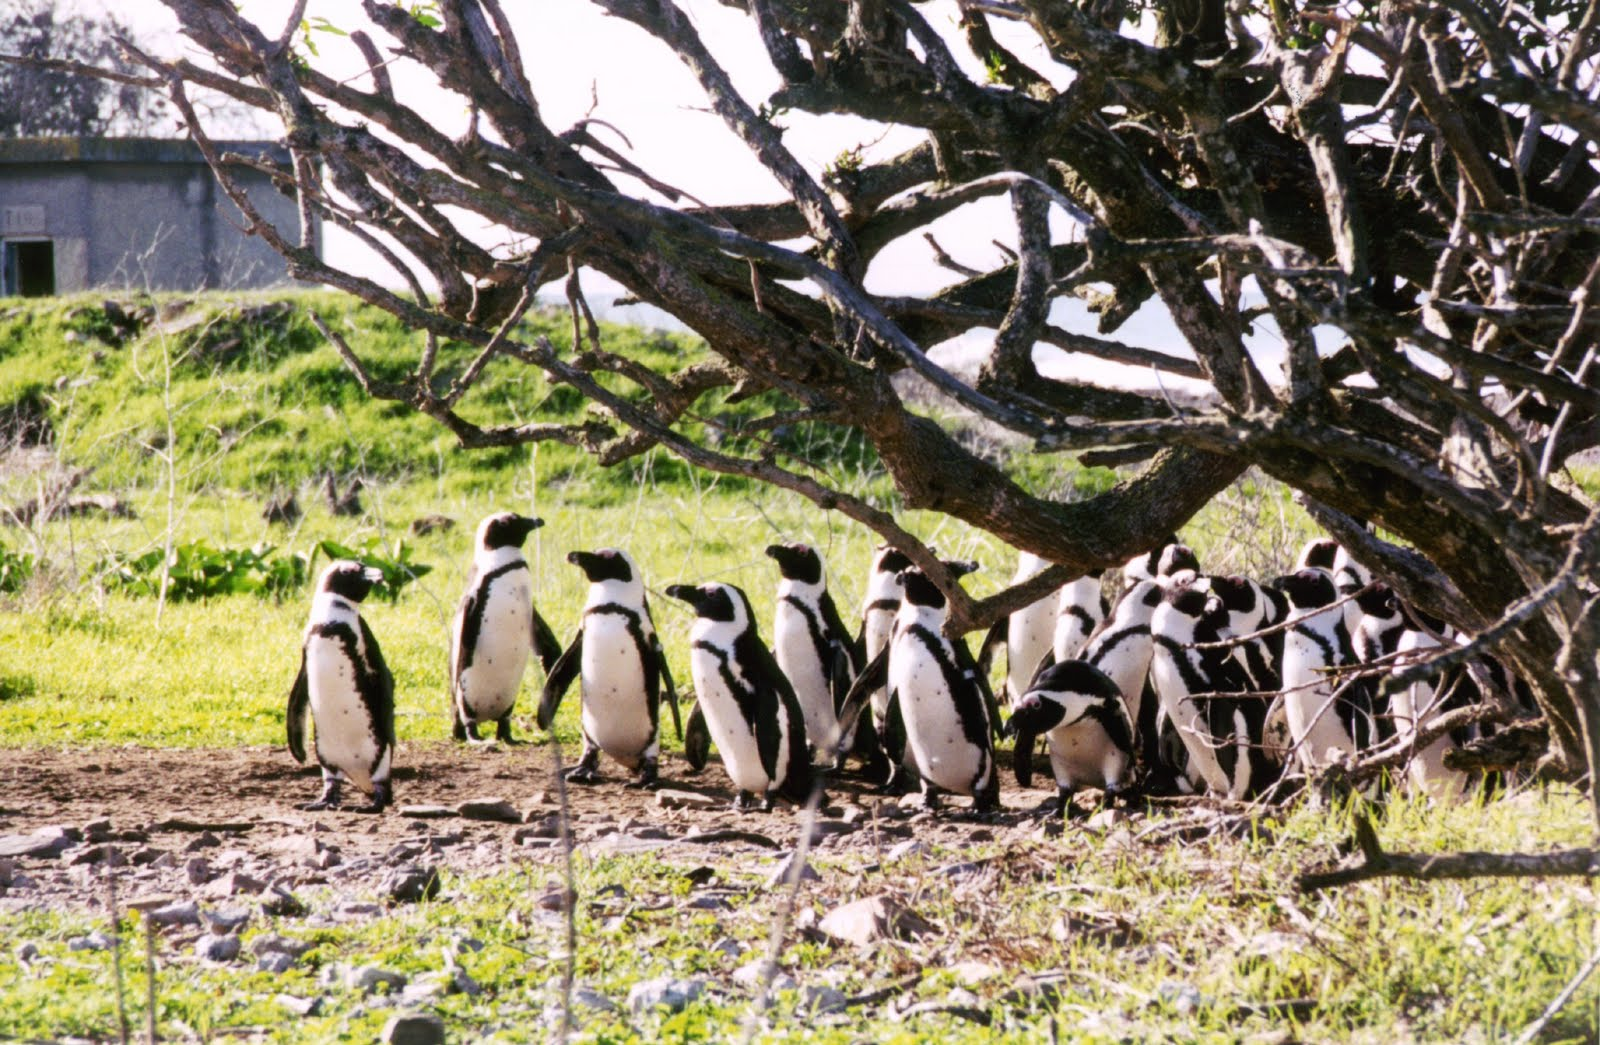
\includegraphics[width=\textwidth]{PenguinTree.jpg}
    \end{column}
  \end{columns}
    \begin{itemize}
    \item Measurements of branching fractions and CPV observables provide tests of standard model and searches for new physics
    \item \textbf{2 \& 4 Body Examples:} Searches for \decay{\PB}{baryon} decays, Angular analysis of \decay{\PB}{VV} decays, time (in)dependent CPV
    \item \textbf{3 Body Examples:} Dalitz analyses and CPV observables, Bc decays, searches for unobserved decays
    \end{itemize}
\end{frame}

\begin{frame}{BnoC Activities}
  \begin{itemize}
  \item \textbf{Currently in review:}
    6 Analyses in WG review, 7 with review committee \& 1 in collaboration wide review
  \item \textbf{Since last \lhcb week:}
    \begin{itemize}
    \item 2 Papers Published:
      \begin{itemize}
      \item $4.1\sigma$ evidence for the decay \decay{\Bp}{\proton \Lbar} (LHCb-PAPER-2016-048)\\
      \item Upper limit on \BF(\decay{\Bs}{\phiz \etapr}) $< 0.82 \times 10^{-6}$ at $90\%$ CL. (LHCB-PAPER-2016-060)
      \end{itemize}
    \item 2 Papers Submitted:
      \begin{itemize}
      \item First observation of a baryonic \Bs decay (LHCB-PAPER-2017-012)
      \item Observation of the charmless baryonic decays \decay{\PB^{0}_{(s)}}{\proton \antiproton h^{+} h^{-}} (LHCb-PAPER-2017-005)
      \end{itemize}
    \end{itemize}
  \item 32 Analyses in preperation - only able to present a few today.
  \item Details of all past and present analyses can be found in the \href{https://lhcb-wg.web.cern.ch/lhcb-WG/bnoc/list.py}{\textcolor{blue}{WG database}}
  \end{itemize}
\end{frame}

\begin{frame}
  \begin{center}
    \begin{block}{}
      \centering \Huge \decay{\PB^{0}_{(s)}}{\proton\antiproton} Update
    \end{block}
    \href{https://lhcb-wg.web.cern.ch/lhcb-WG/bnoc/listentry.py?name=2011\%2B12+B+-\%3E+p+pbar+BFs\&cat=analysis}{\textcolor{blue}{Link to WG Database}}
  \end{center}
\end{frame}

\begin{frame}{\decay{\PB^{0}_{(s)}}{\proton\antiproton} Motivation and Status}
  \begin{block}{Motivation}
    \begin{itemize}
    \item No baryonic 2 body charmless $\PB^{0}$ decay has been observed.
    \item \decay{\PB^{0}_{(s)}}{\proton\antiproton} decays predicted to be simplest to search for experimentally
    \end{itemize}
  \end{block}
  \begin{itemize}
  \item Previous analysis using 2011 data saw $3.3\sigma$ evidence for \decay{\Bd}{\proton\antiproton} but no evidence for the suppressed \decay{\Bs}{\proton\antiproton} seen.
  \item Hopefully addition of 2012 data can lead to an observation.
  \end{itemize}
  \begin{columns}
    \begin{column}{0.65\textwidth}
      \begin{itemize}
      \item Branching fraction results using 2011 data: \\
        \BF(\decay{\Bd}{\proton\antiproton})$ = (1.47^{+0.62+0.35}_{-0.51-0.14})\times 10^{-8}$\\
        \BF(\decay{\Bs}{\proton \antiproton})$ = (2.84^{+2.03 +0.85}_{-1.68 -0.18}) \times 10^{-8}$
      \item All previous theory calculations ruled out by at least 1 order of magnitude!
      \end{itemize}
    \end{column}
    \begin{column}{0.34\textwidth}
      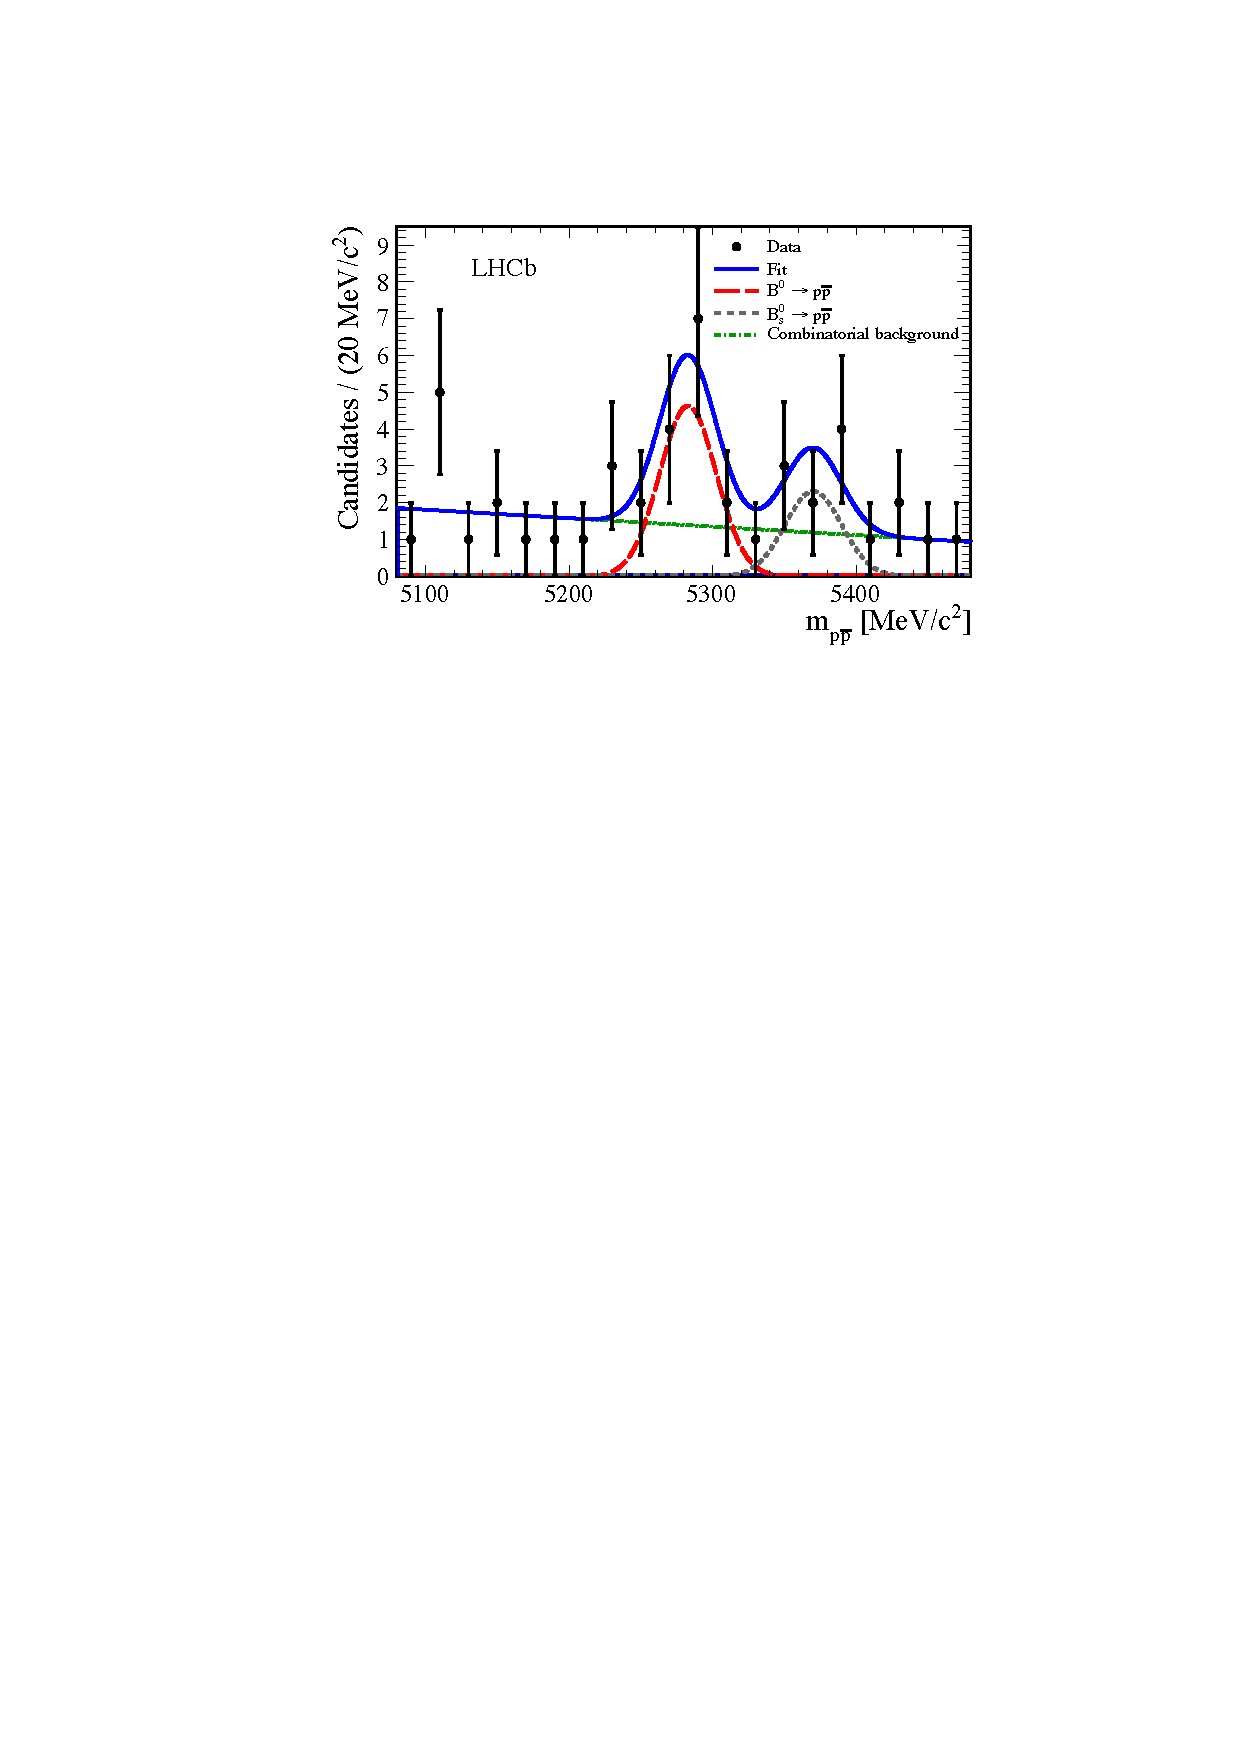
\includegraphics[width=\textwidth]{2011PPbar.pdf}
    \end{column}
  \end{columns}
\end{frame}

\begin{frame}{Selection}
  \small
  \begin{itemize}
  \item PID Selection optimises \dllppi and \dllpk cuts for Punzi FoM with $a=5\sigma$
  \item MVA selection (applied after PID selection) makes use of MLP with 10 variables, again optimised for Punzi FoM.
    \begin{center}
      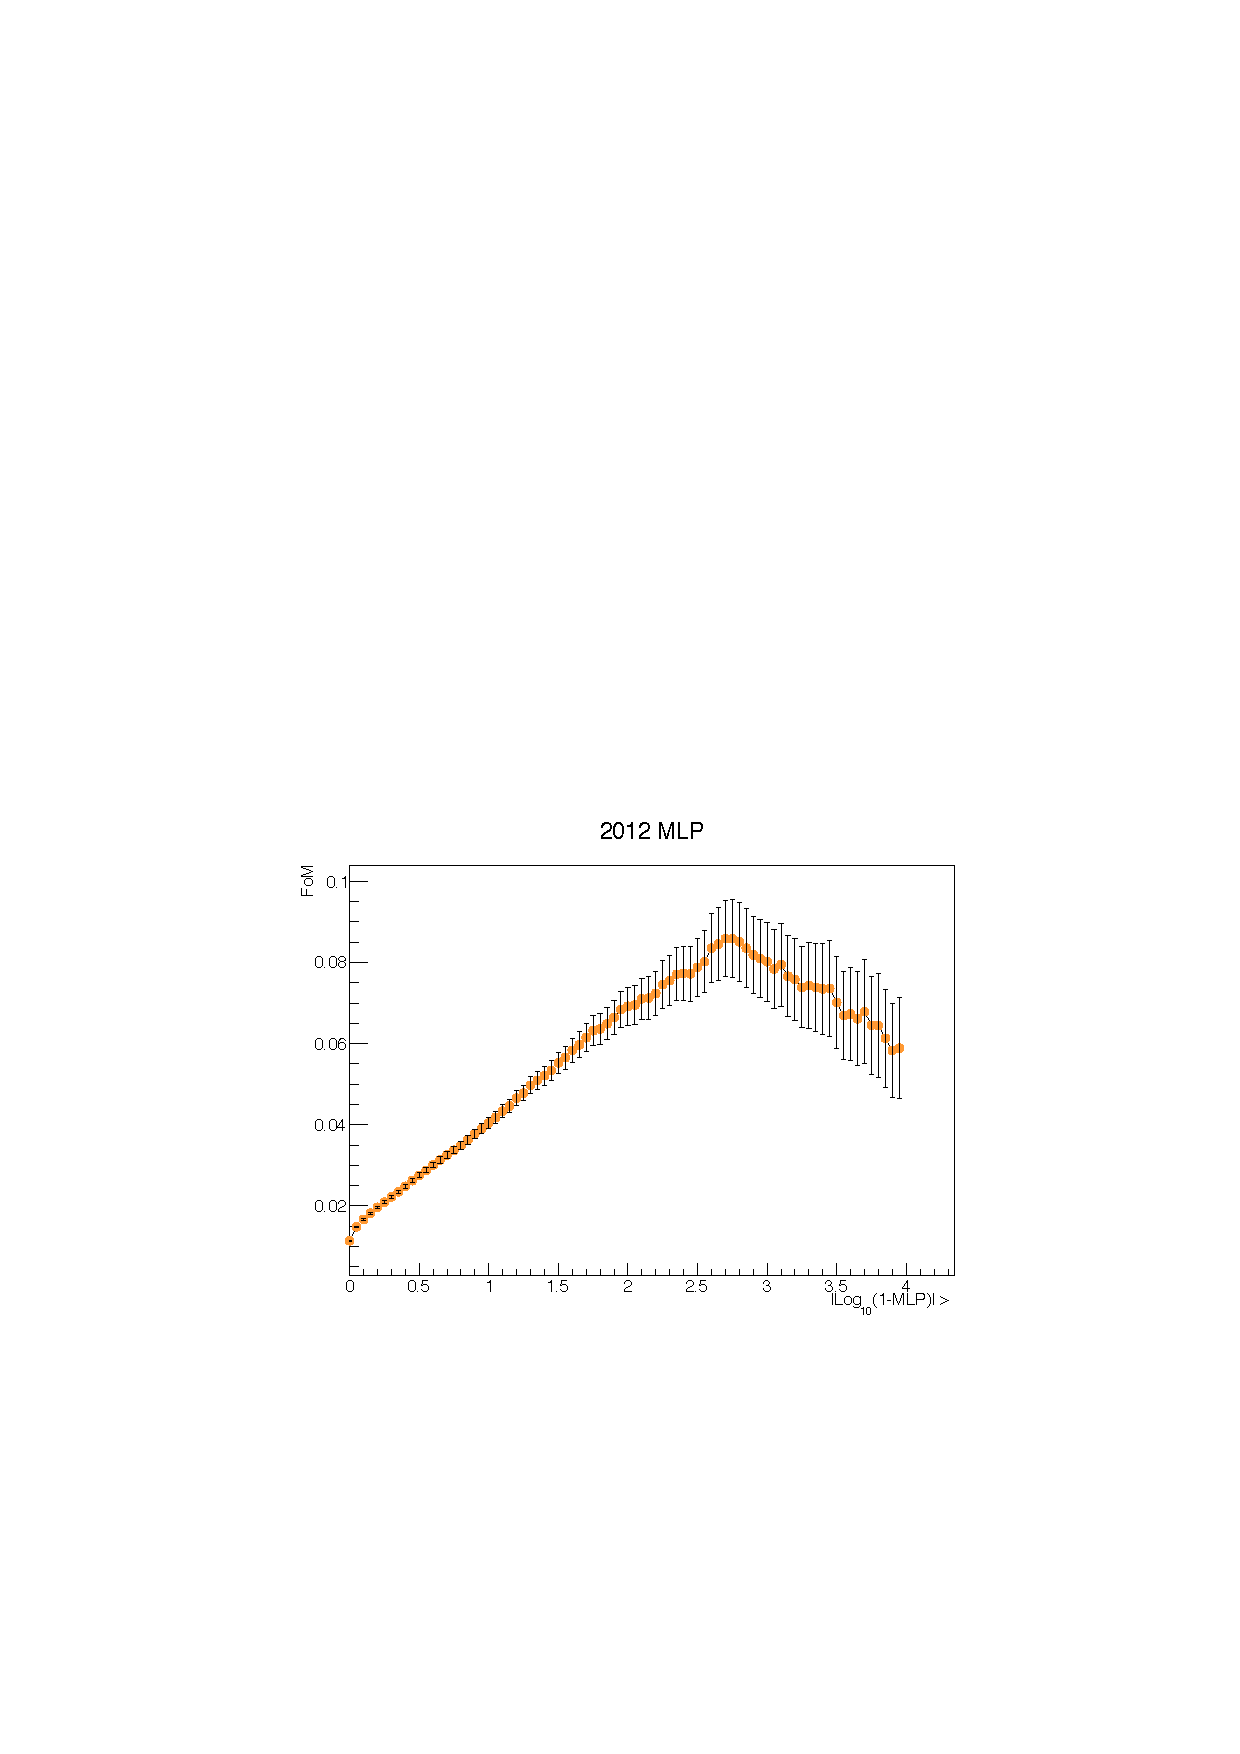
\includegraphics[width=.4\textwidth]{PPOptimisation.pdf}
      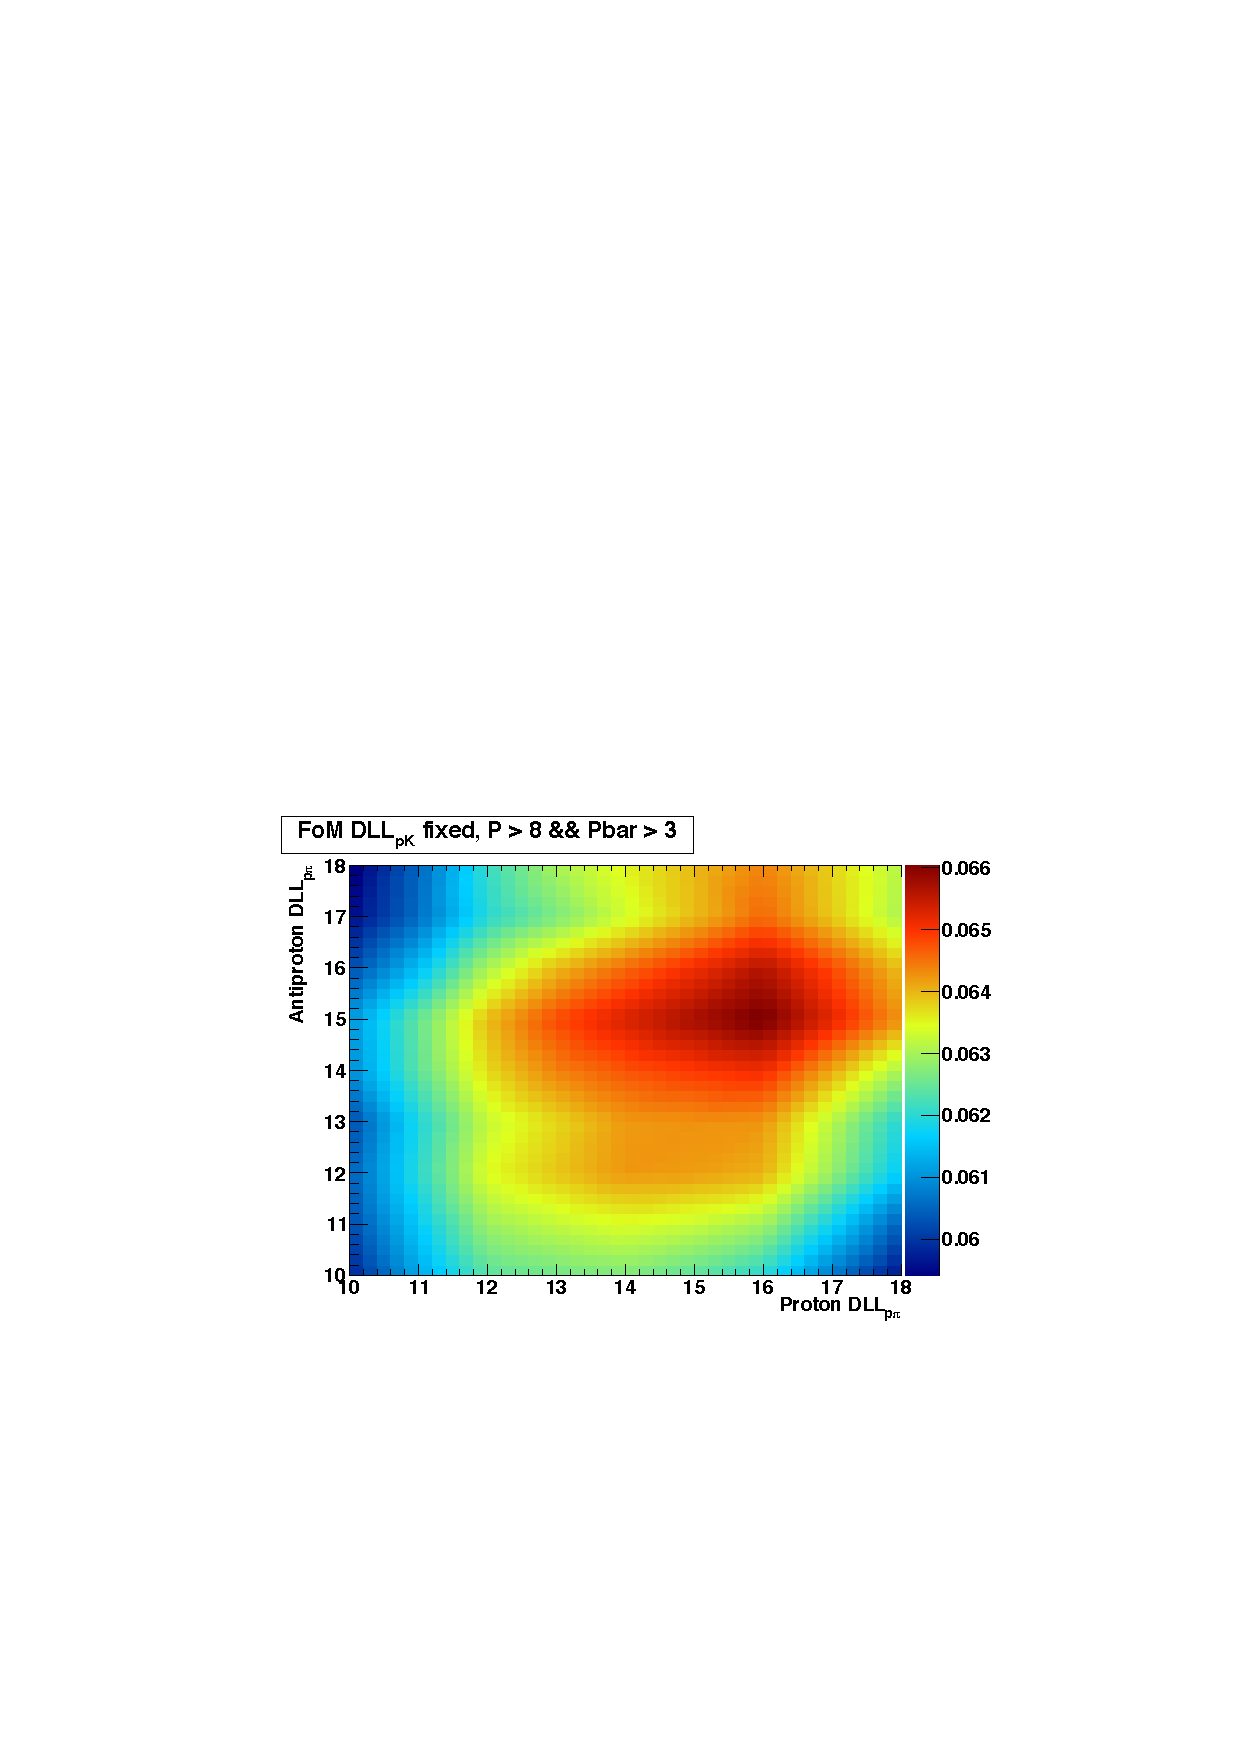
\includegraphics[width=.4\textwidth]{PPBarPIDOptimisation.pdf}
    \end{center}
  \item Normalisation channel, \decay{\Bd}{\Kp\pim}, PID selection optimised for maximum selection efficiency whilst rejecting various mis-ID backgrounds.    % READ.
  \item Similar MLP also used in normalisation channel, but optimised for signal significance.
  \end{itemize}
\end{frame}

\begin{frame}{Fits}
  \small
  \begin{itemize}
  \item \textbf{Normalisation channel:} Mass fit seperated by charge due to known production assymmetries
  \begin{center}
    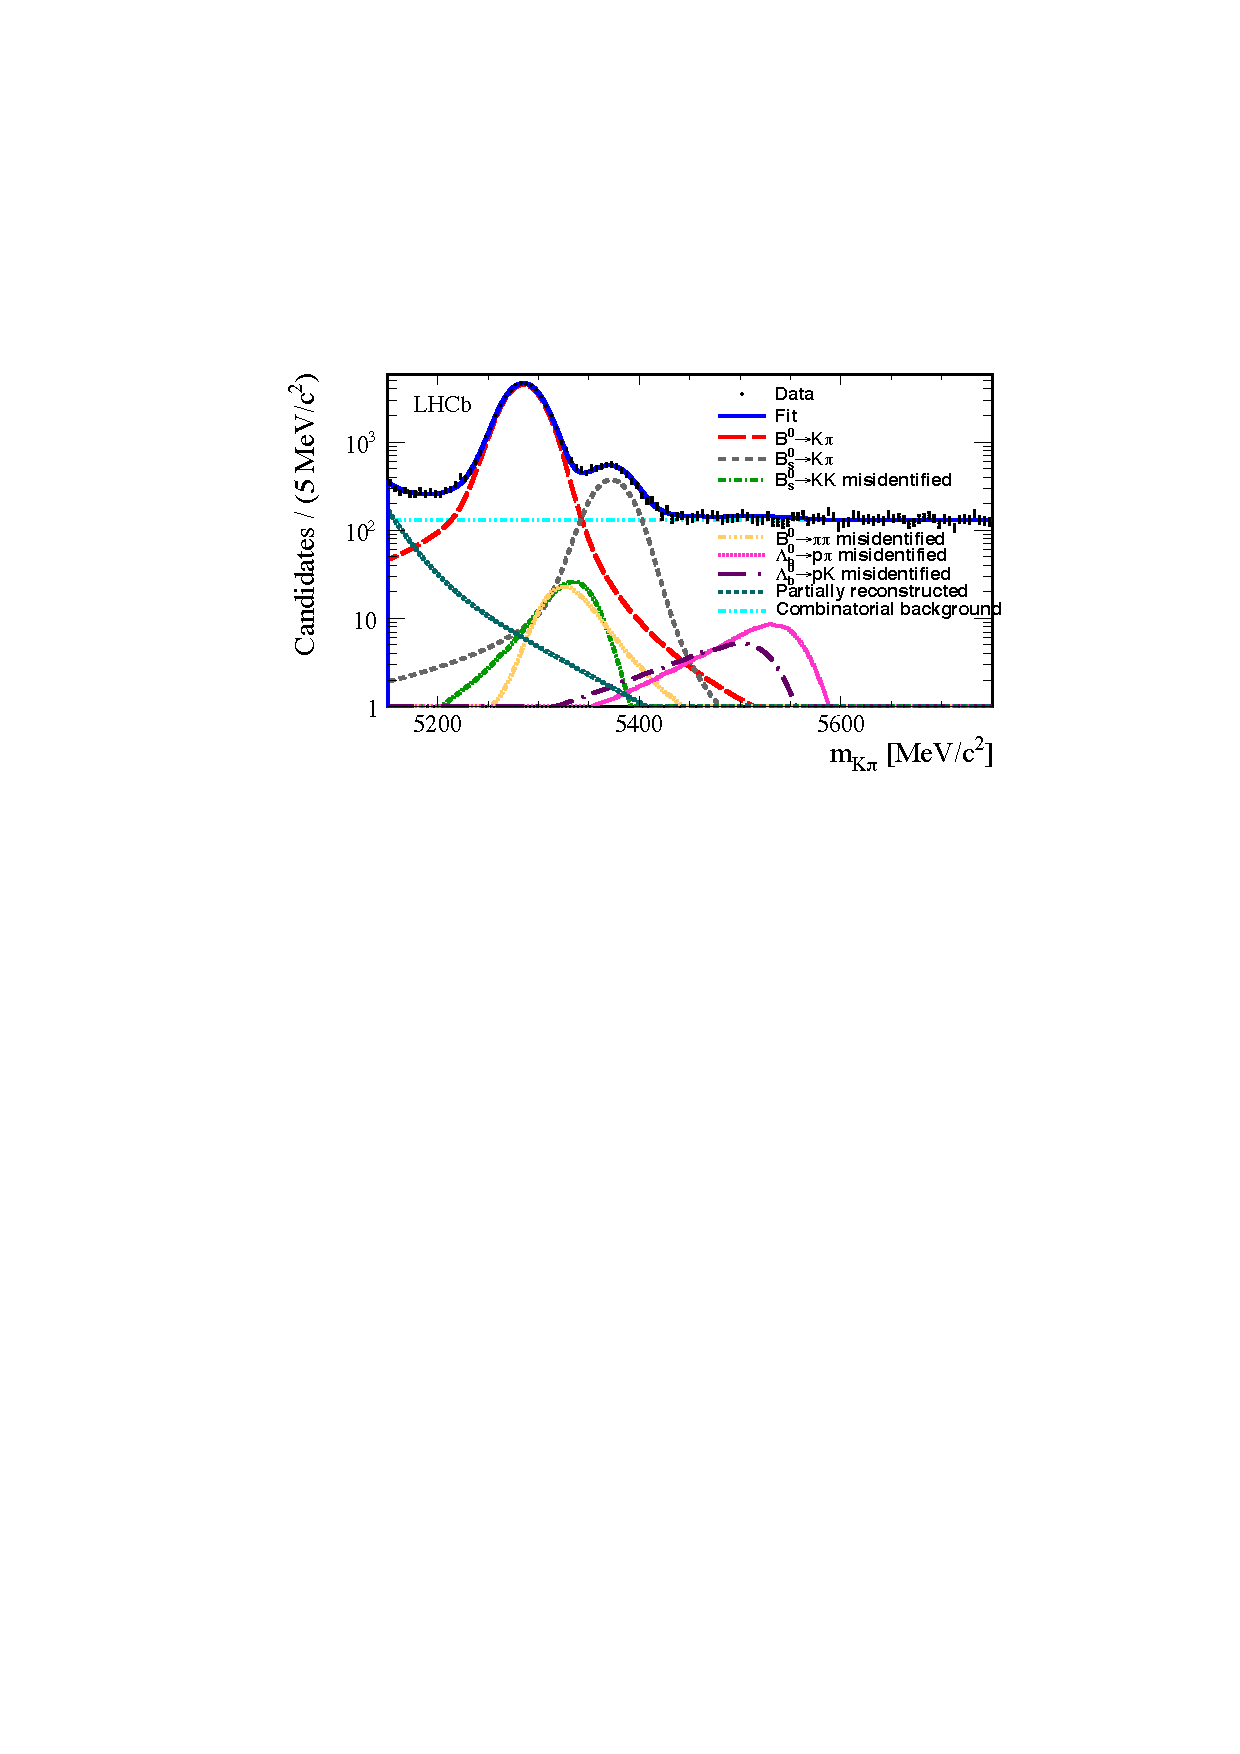
\includegraphics[width=0.32\textwidth]{PPNormMassFit.pdf}
    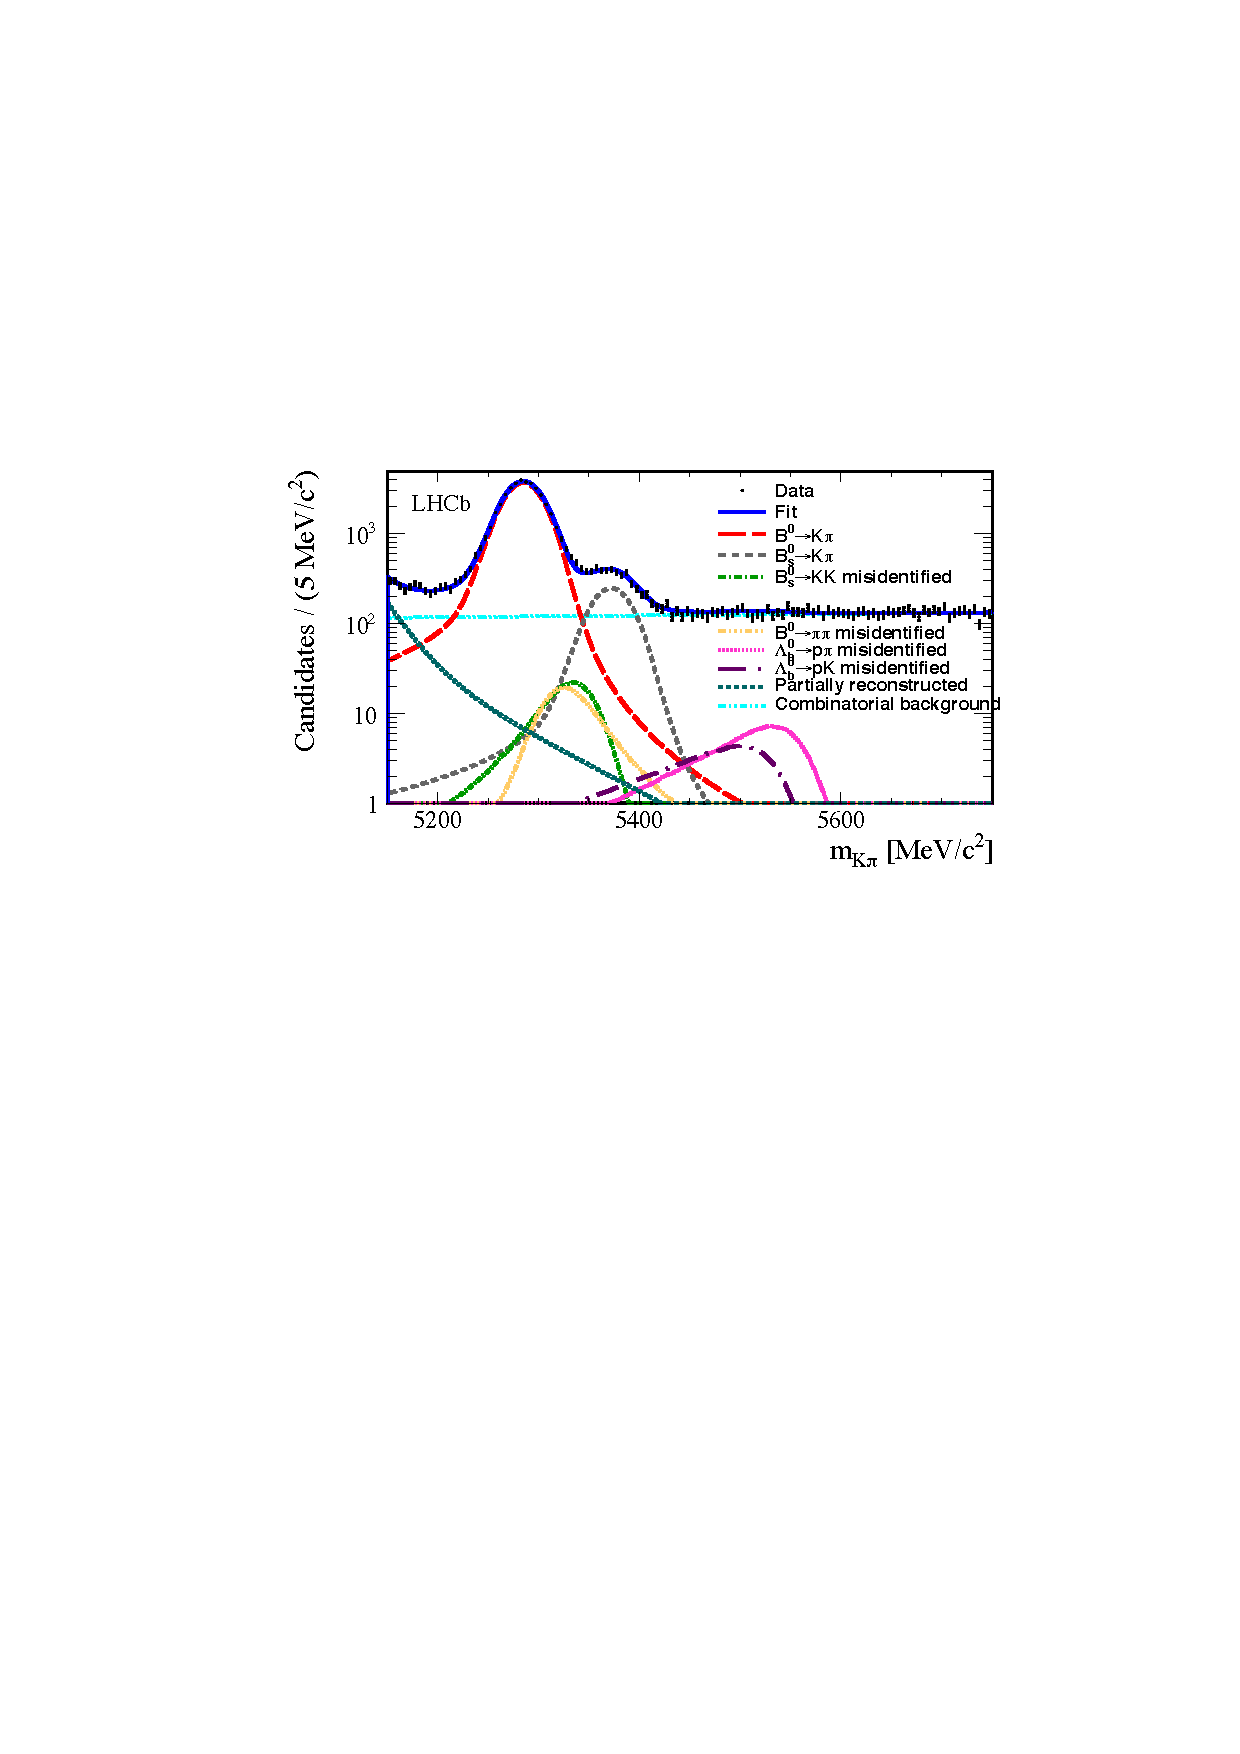
\includegraphics[width=0.32\textwidth]{PPNormMassFitBar.pdf}
  \end{center}
  \item \textbf{Signal channel:} Only signal and combinatorial background present - $38.7\pm8.4(stat only)$ \decay{\Bd}{\proton\antiproton} decays observed!
    % \item $N(\decay{\Bd}{\proton\antiproton} = 38.7\pm8.4 (stat only)$ and $N(\decay{\Bs}{\proton\antiproton} = 1.5\pm4.4 (stat only)$.
    \begin{center}
      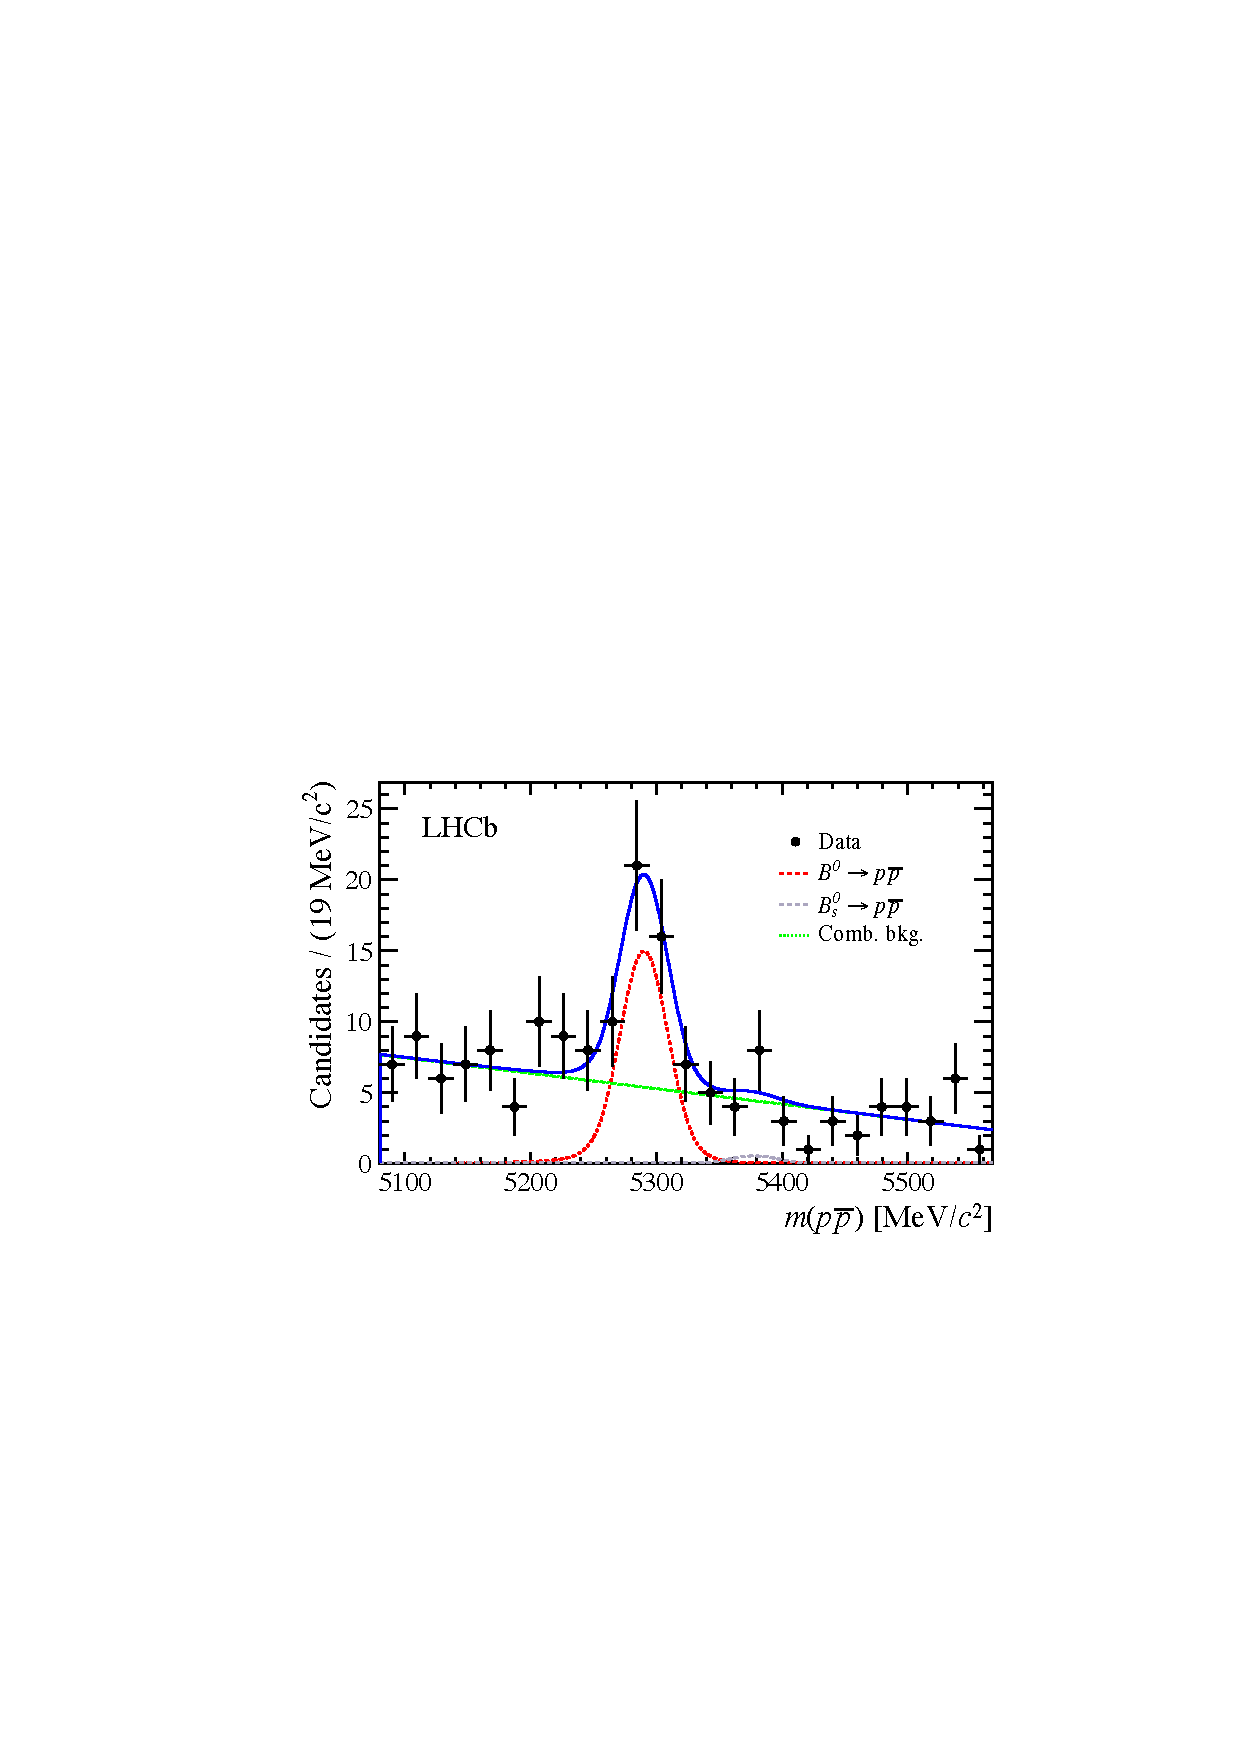
\includegraphics[width=.4\textwidth]{PPSignalMassFit.pdf}
    \end{center}
  \end{itemize}
\end{frame}

\begin{frame}{Results and Outlook}
  \begin{itemize}
  \item First obeservation of \decay{\Bd}{\proton \antiproton} with significance of $5.3\sigma$ -first obseration of 2 body charmless baryonic \Bd decay!
  \item \BF(\decay{\Bd}{\proton \antiproton})$ = (1.25\pm0.27\pm0.18) \times 10^{-8}$.
  \item \decay{\Bs}{\proton \antiproton} yield of only $1.5\pm4.4$ events, limit set using Feldman-Cousins method.
    \begin{center}
      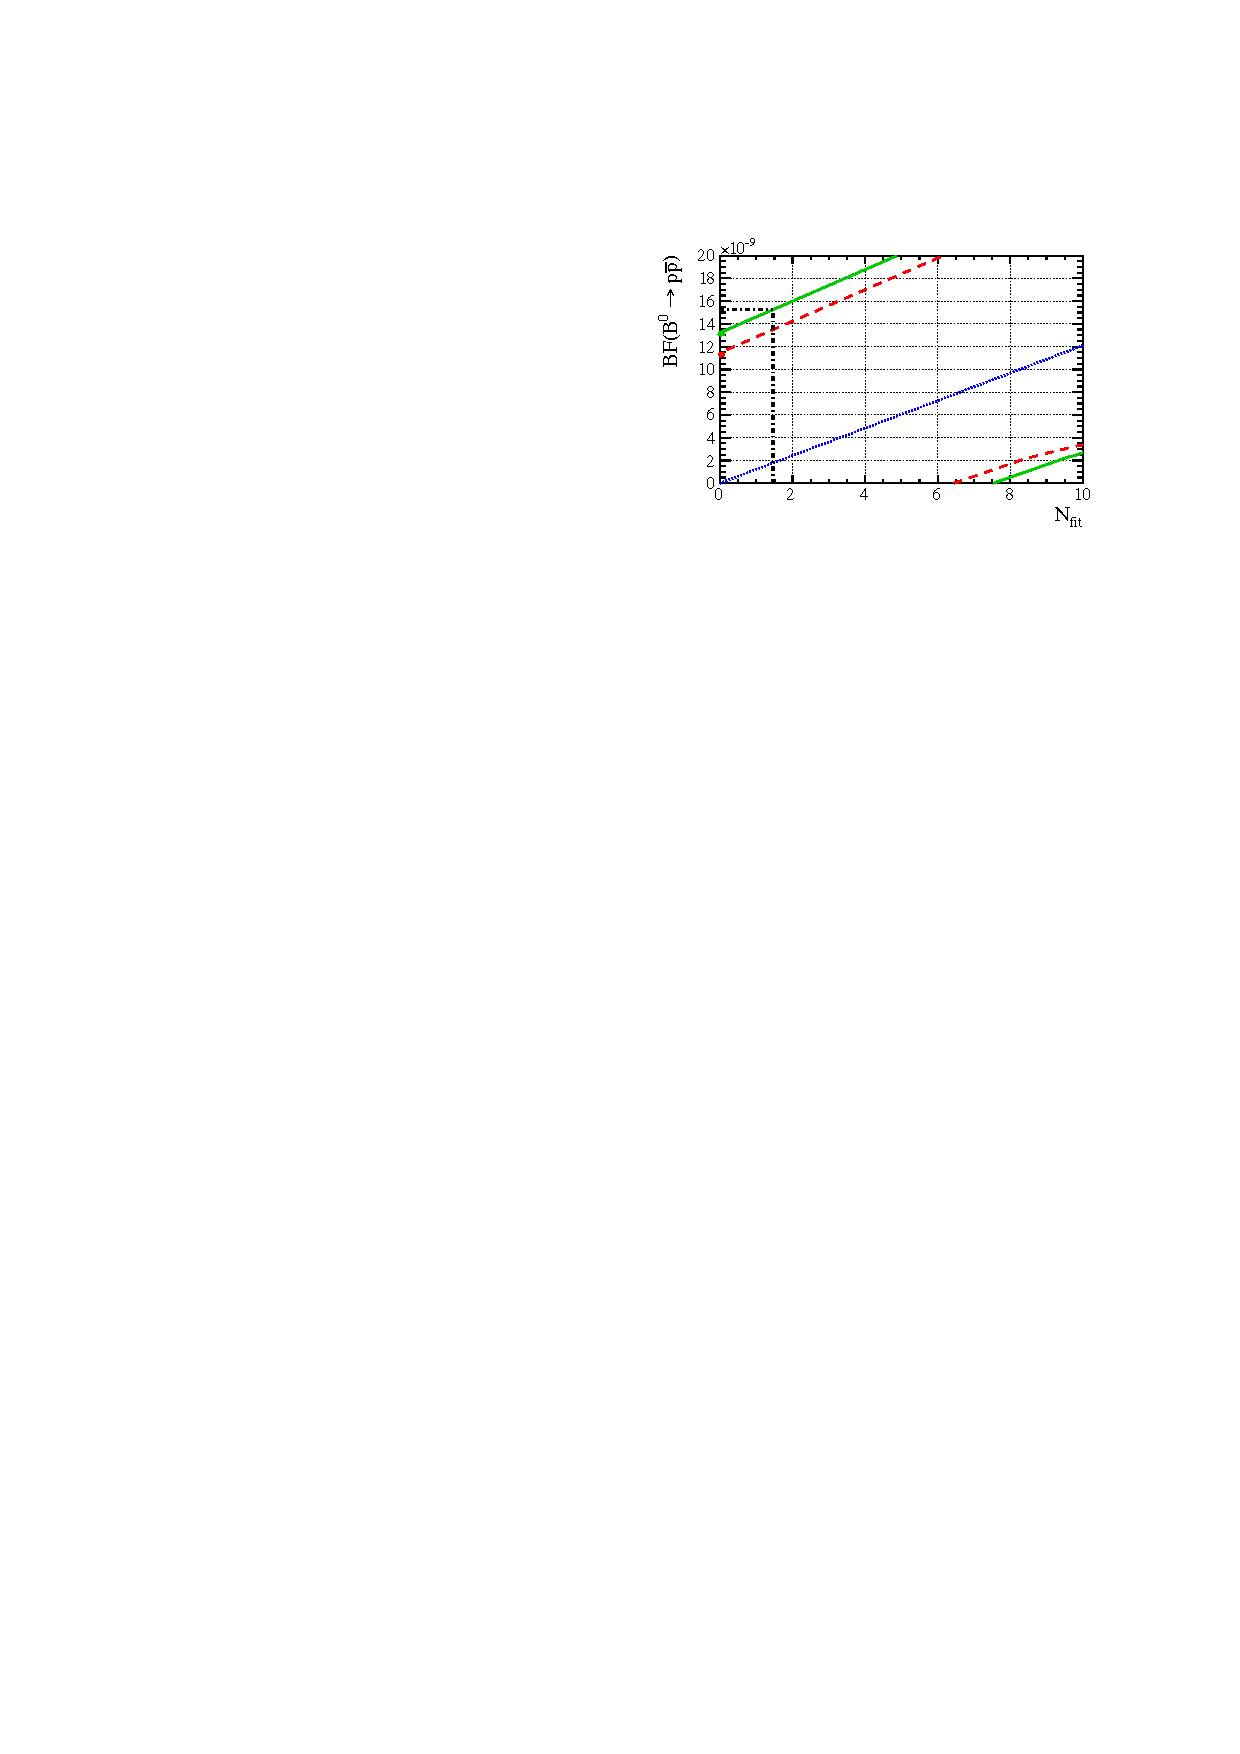
\includegraphics[width=0.4\textwidth]{PPBarFC.pdf}
    \end{center}
  \item \BF(\decay{\Bs}{\proton \antiproton})$ < 1.5 \times 10^{-8} $ at $90\%$ confidence level.
  \item Analysis close to publication, paper currently in collaboration wide review.
  \end{itemize}
\end{frame}

\begin{frame}
  \begin{block}{}
    \centering Amplitude analysis of \Large \decay{\Bd}{(\pip \pim)(\Kp\pim)} decays
  \end{block}
  \centering \href{https://lhcb-wg.web.cern.ch/lhcb-WG/bnoc/listentry.py?name=2011\%2B12+B+-\%3E+K\%2A0+rho0+BF\&cat=analysis}{\textcolor{blue}{Link to WG database}}
\end{frame}

\begin{frame}{The \decay{\Bd}{\rhoz(\pi \pi)\Kstarz(\Kp\pim)} decay}
  \begin{columns}
    \begin{column}{.75\textwidth}
      \begin{itemize}
        \item Proceeds either via:
        \begin{itemize}
        \item A doubly Cabibbo suppressed tree
        \item A gluonic \decay{\bquark}{\squark} penguin
        \item Both have similar amplitudes, good for $a_{cp}$!
        \end{itemize}
      \item Self tagged decay: \\ \decay{\textcolor{red}{\Bd}}{\rhoz(\pi \pi)\Kstarz(\textcolor{red}{\Kp}\pim)} \\ \decay{\textcolor{red}{\Bdb}}{\rhoz(\pi \pi)\Kstarz(\textcolor{red}{\Km}\pip)}
      \item \textbf{Aim:} Measure longitudinal polarisation fraction $f_L$, \ACP and accessible triple product assymmetries.
      \item Amplitude analysis required to disentangle different helicity amplitudes and final states.
      \end{itemize}
    \end{column}
    \begin{column}{.24\textwidth}
      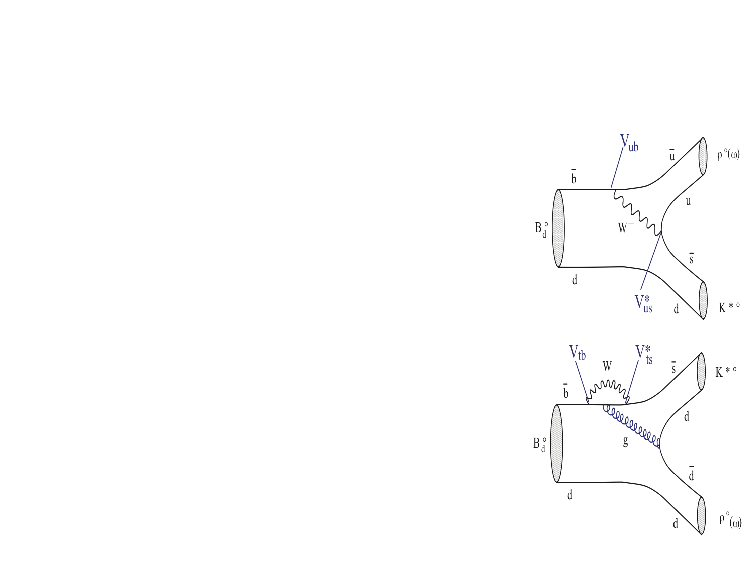
\includegraphics[width=\textwidth]{KstarRhoFeynman.pdf}
    \end{column}
  \end{columns}
\end{frame}

\begin{frame}{Event Selection}
  \begin{itemize}
  \item A BDT is used to reject combinatorial background, cut chosen rejects $~99\%$ of background samples whilst retaining $\geq90\%$ of signal MC.
  \item Charm resonances removed with vetoes
  \item Tight PID cuts remove most mis-ID backgrounds. \\ \vspace{0.2cm}
    \begin{columns}
      \begin{column}{0.6\textwidth}
        \textbf{\decay{\Bs}{\Kstarz\Kstarzb} background:}
        \begin{itemize}
        \item PID cuts modified to create seperate sample with high purity of these events, M(\kaon\pion\kaon\pion) fitted to determine level of contamination.
        \item Simulated \decay{\Bs}{\Kstarz\Kstarzb} events injected with negative weights to remove \decay{\Bs}{\Kstarz(\Km\pip)\Kstarzb(\Kp\pim)} background.
        \end{itemize}
      \end{column}
      \begin{column}{0.39\textwidth}
        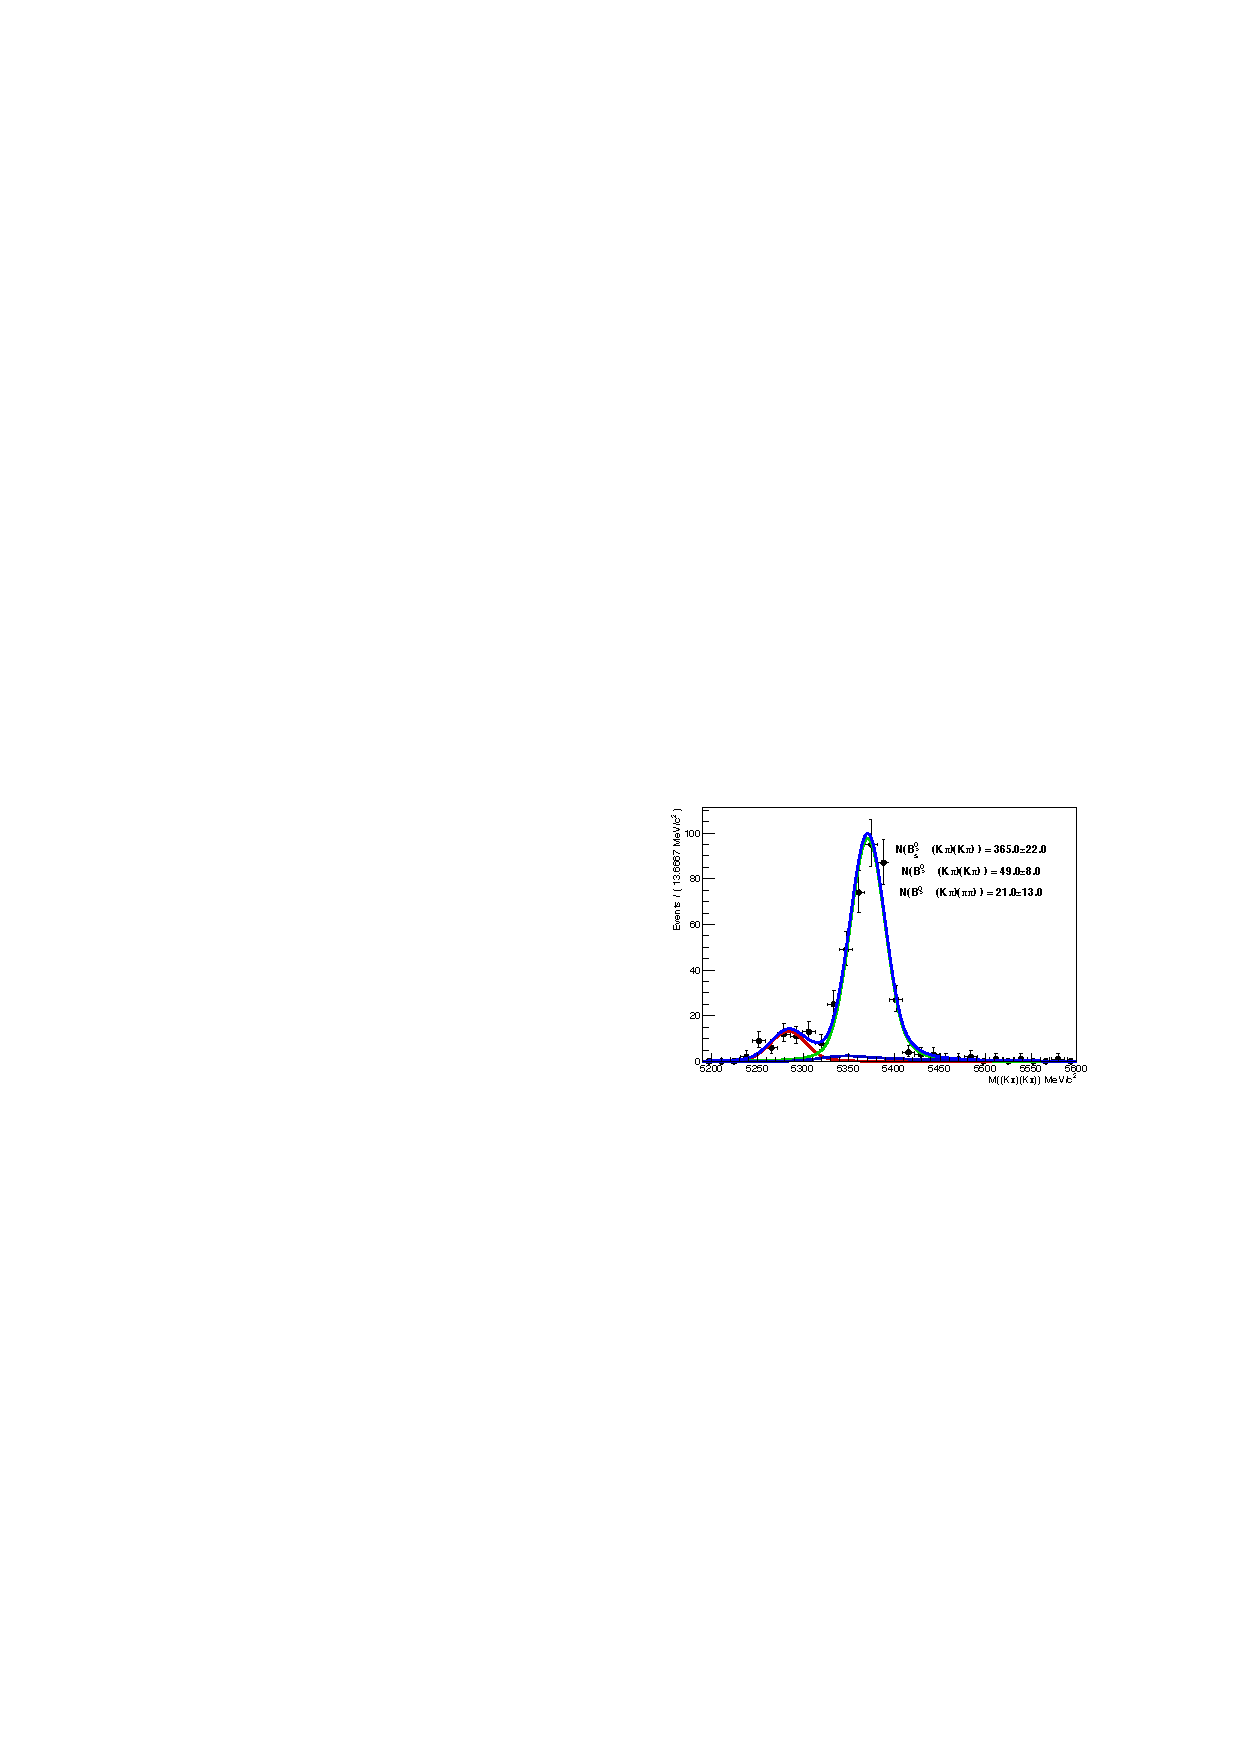
\includegraphics[width=\textwidth]{KstarKstarSelection.pdf}
      \end{column}
    \end{columns}
  \end{itemize}
\end{frame}

\begin{frame}{Four Body Mass Fit}
  \begin{itemize}
  \item \textbf{Aim: Perform fit to M(\pion\pion\kaon\pion) distribution and extract sWeights}
  \item \decay{\PB^{0}_{(s)}}{(\Kp\pim)(\pip\pim)} peaks modelled with Hypatia function, combinatorial background modelled with exponential.
    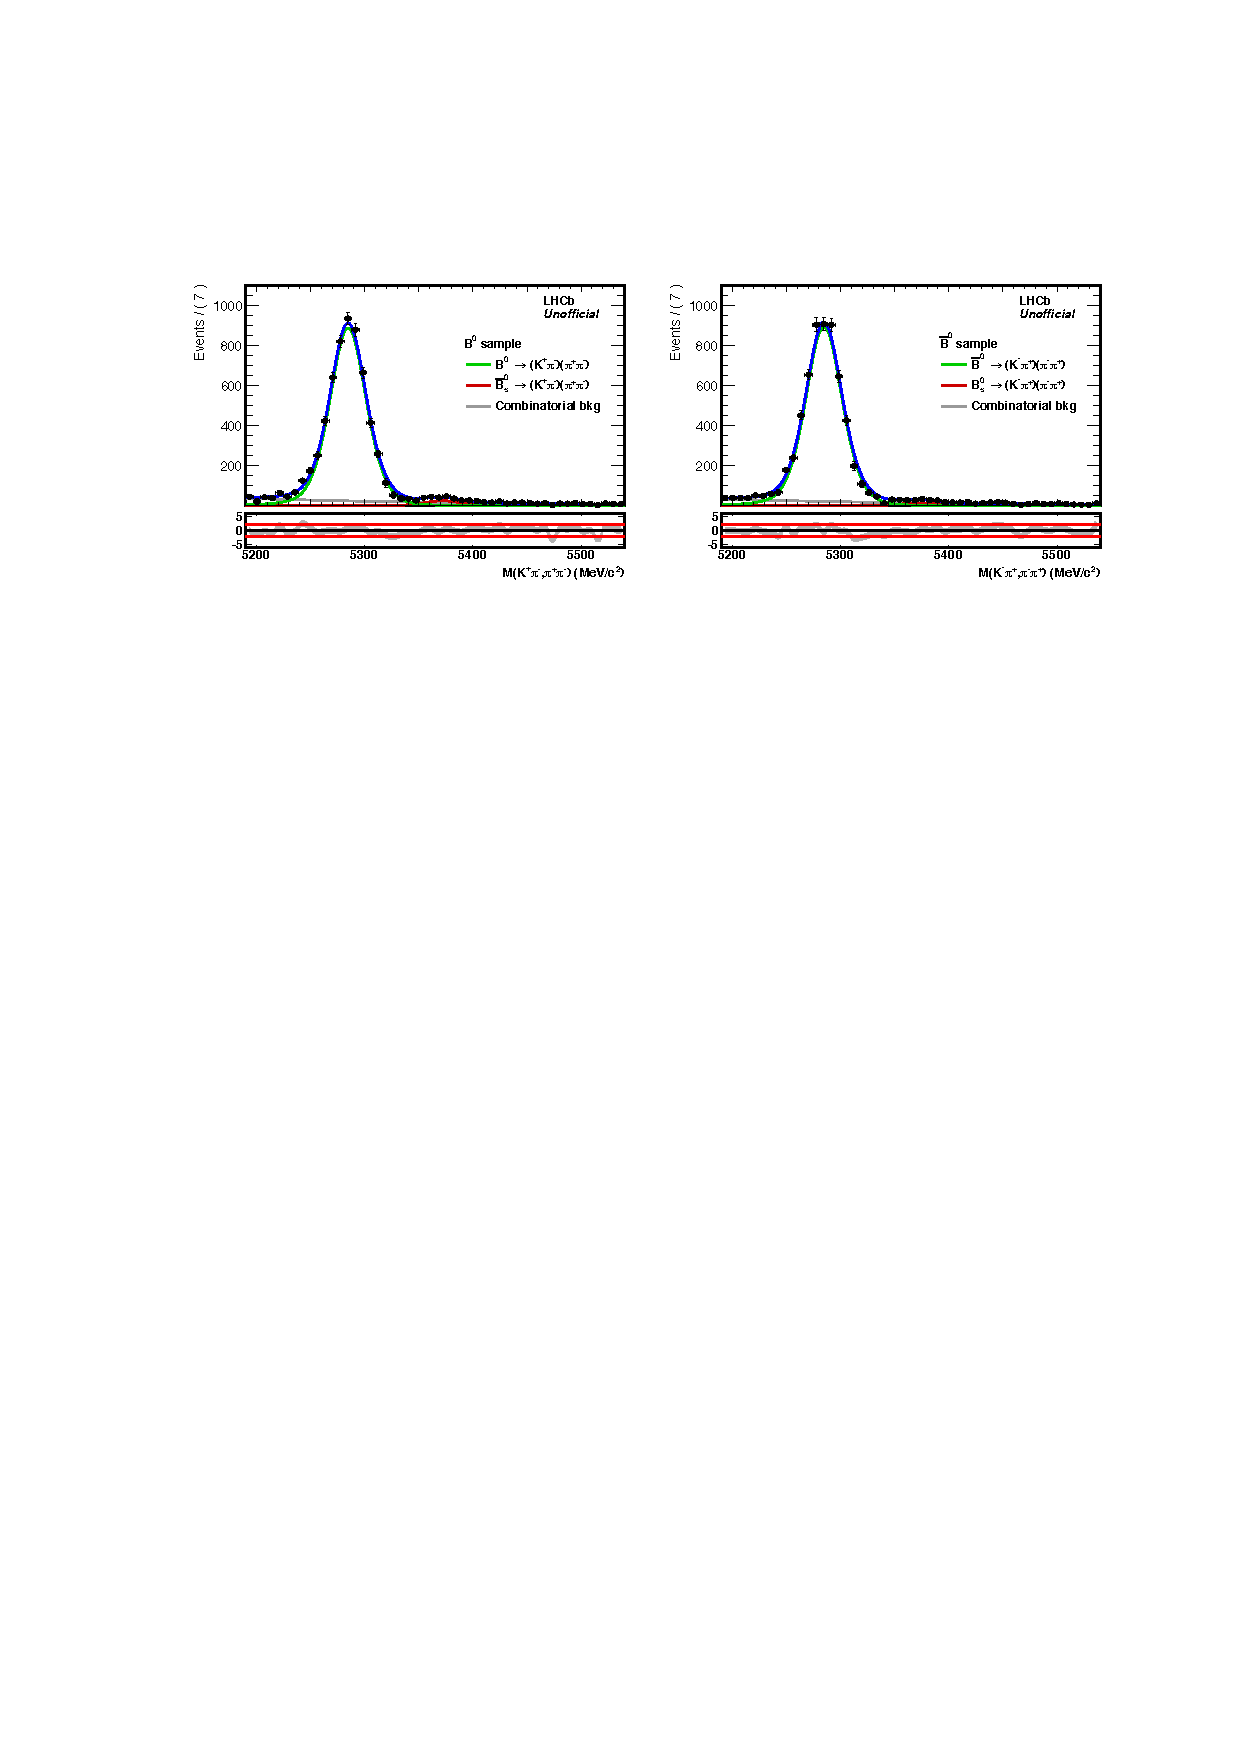
\includegraphics[width=.9\textwidth]{KstarRho4Bod.pdf}
  \item Total of 11290 \decay{\Bd}{(\pip\pim)(\Kp\pim)} signal events.
  \end{itemize}
\end{frame}

\begin{frame}{Amplitude Analysis Formalism}
  \begin{itemize}
  \item Isobar model used to paramaterise the total \decay{\Bd}{(\pip\pim)(\Kp\pim)} decay amplitude:
    \begin{equation}
      A_{T}=\sum_i A_i \times g_i(\theta_{\pip\pim},\theta_{\Kp\pim},\phi) \times M_i(m_{\pip\pim},m_{\Kp\pim})
    \end{equation}
  \item $g_i$ are the legendre polynomials describing the angular distributions
  \item $M_i(\pip\pim,\Kp\pim)$ are functions to model the effective two body masses.
  \end{itemize}
  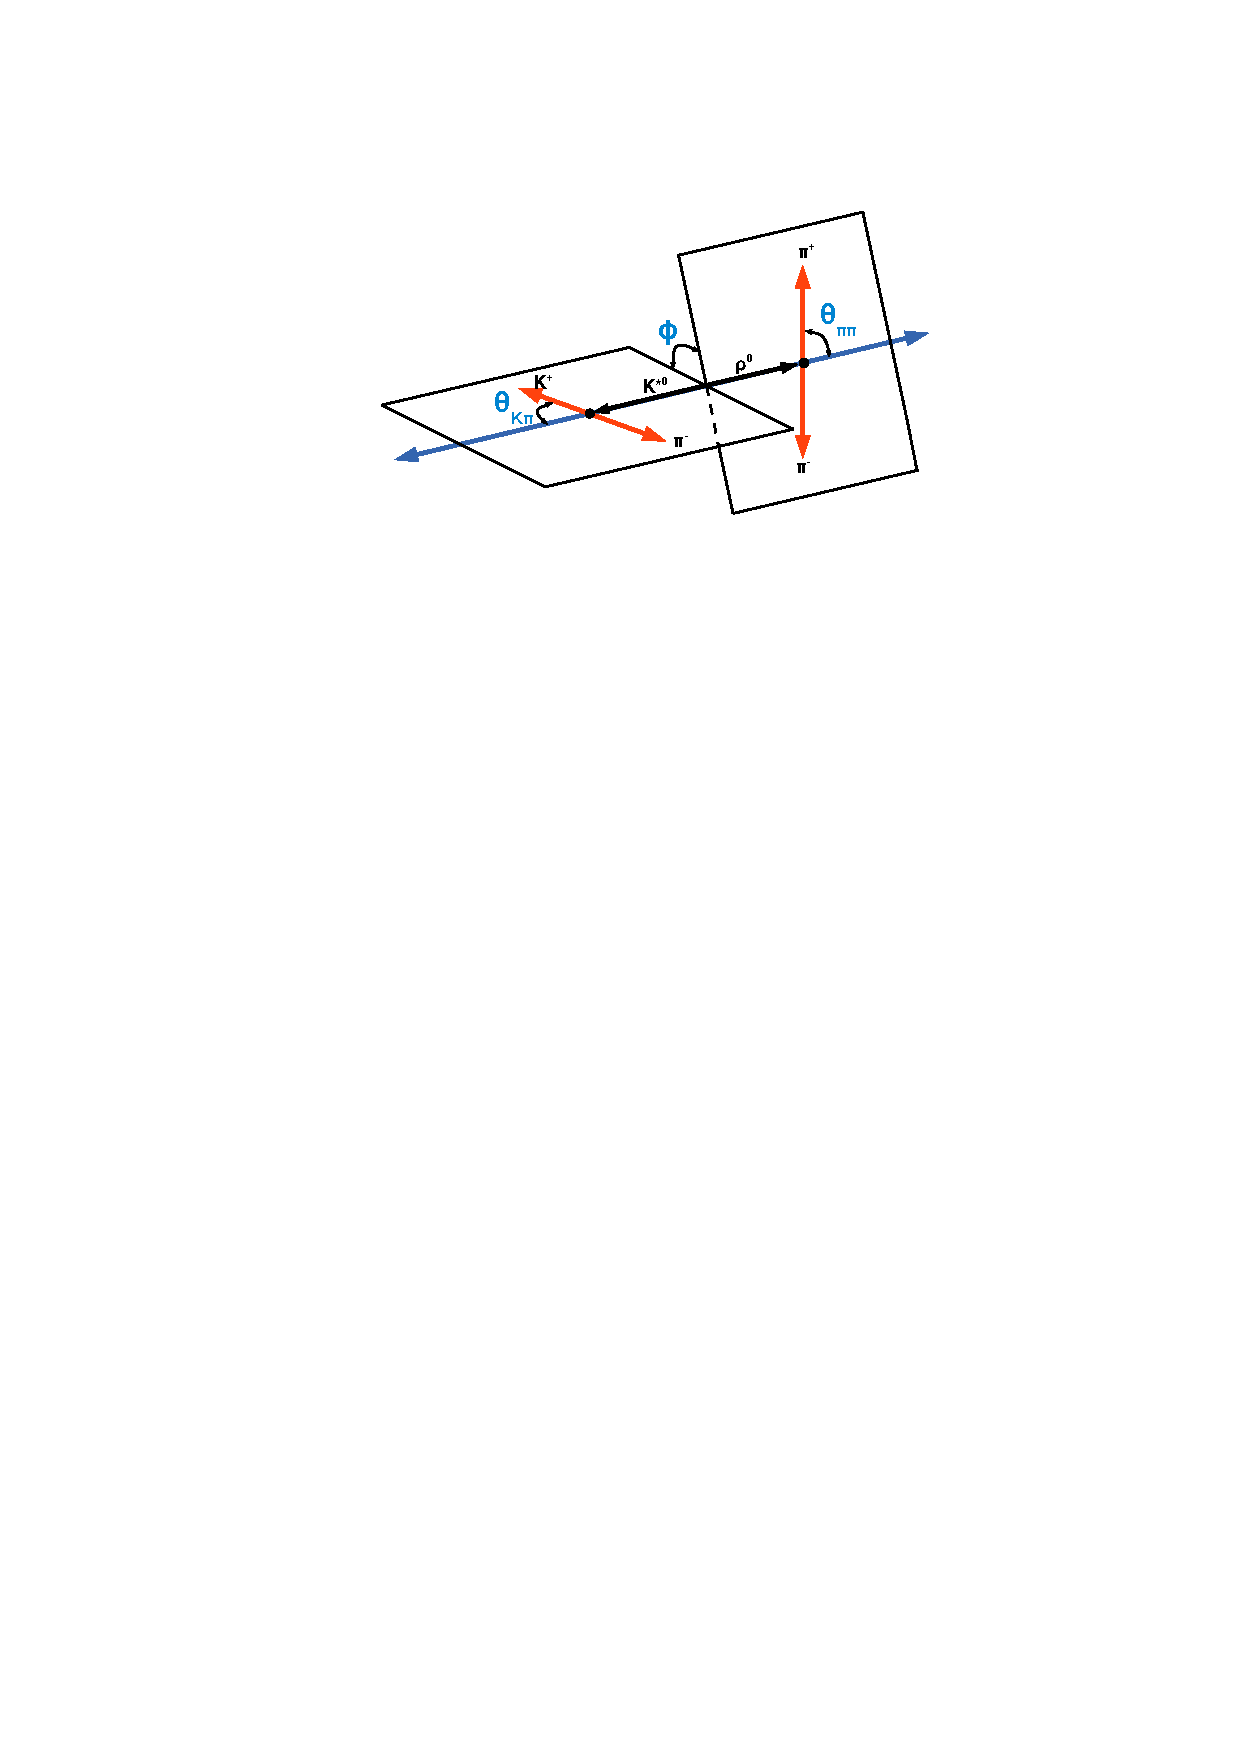
\includegraphics[width=.5\textwidth]{KstarRhozAngles.pdf}
\end{frame}

\begin{frame}{Amplitude Fit}
  \scriptsize
  \begin{itemize}
  \item A PDF has been created to model 11 decay channels and 14 amplitudes.
  \end{itemize}
  \begin{columns}
    \begin{column}{0.3\textwidth}
      \textbf{Nominal Mass Propogators:}
      \begin{itemize}
      \item \textcolor{red}{\Kstarz, \Pomega, $f_0(500)$,$f_0(1370)$:}\\
        Relativistic Breit-Wigner
      \item \textcolor{red}{\rhoz:}\\
        Gounaris-Sakurai
      \item \textcolor{red}{$f_0(980)$:}\\
        Flatte
      \item \textcolor{red}{$(\kaon\pion)_0$}\\
        LASS
      \end{itemize}
    \end{column}
    \begin{column}{0.69\textwidth}
      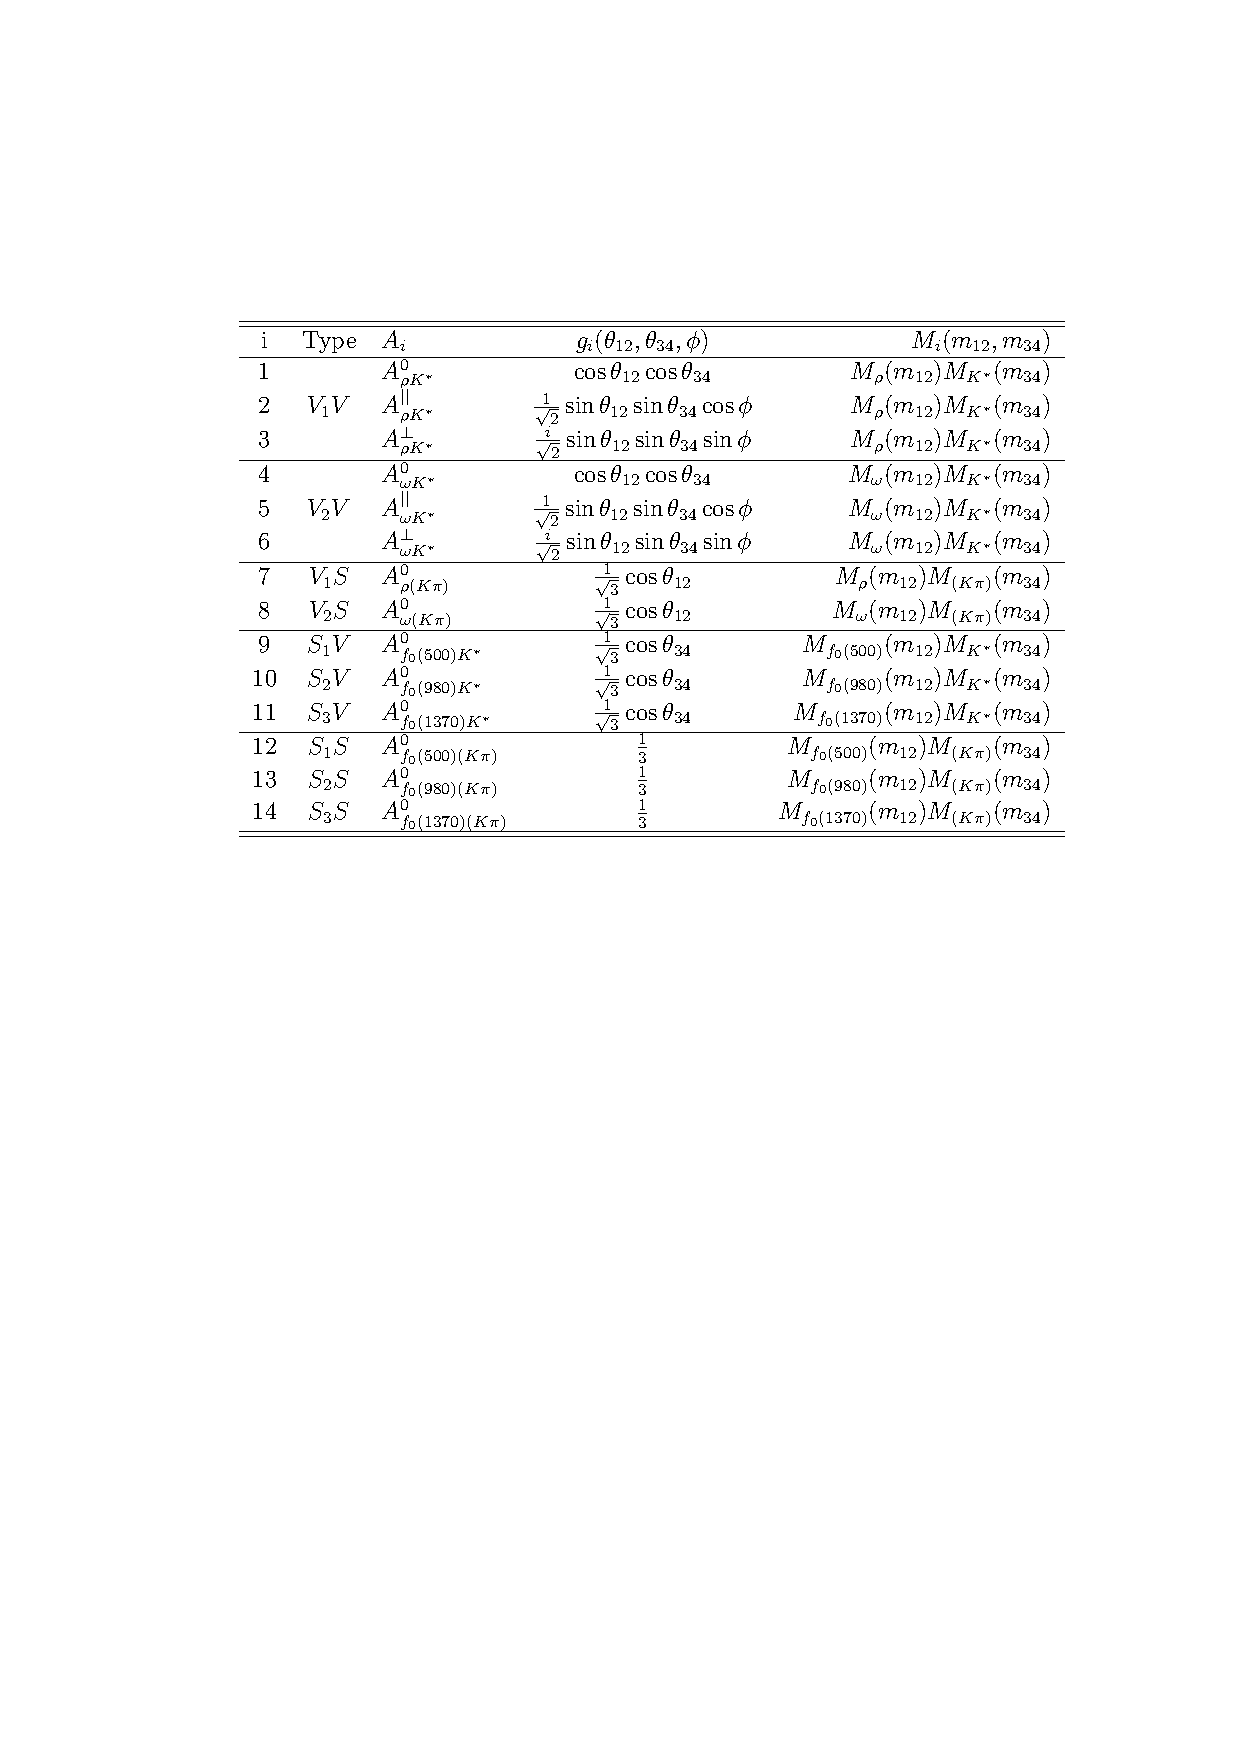
\includegraphics[width=\textwidth]{KstarRhoAmplitudes.pdf}
    \end{column}
  \end{columns}
  \begin{itemize}
  \item Detector acceptance accounted for with normalisation weights
  \end{itemize}
\end{frame}

\begin{frame}{Results and Outlook}
  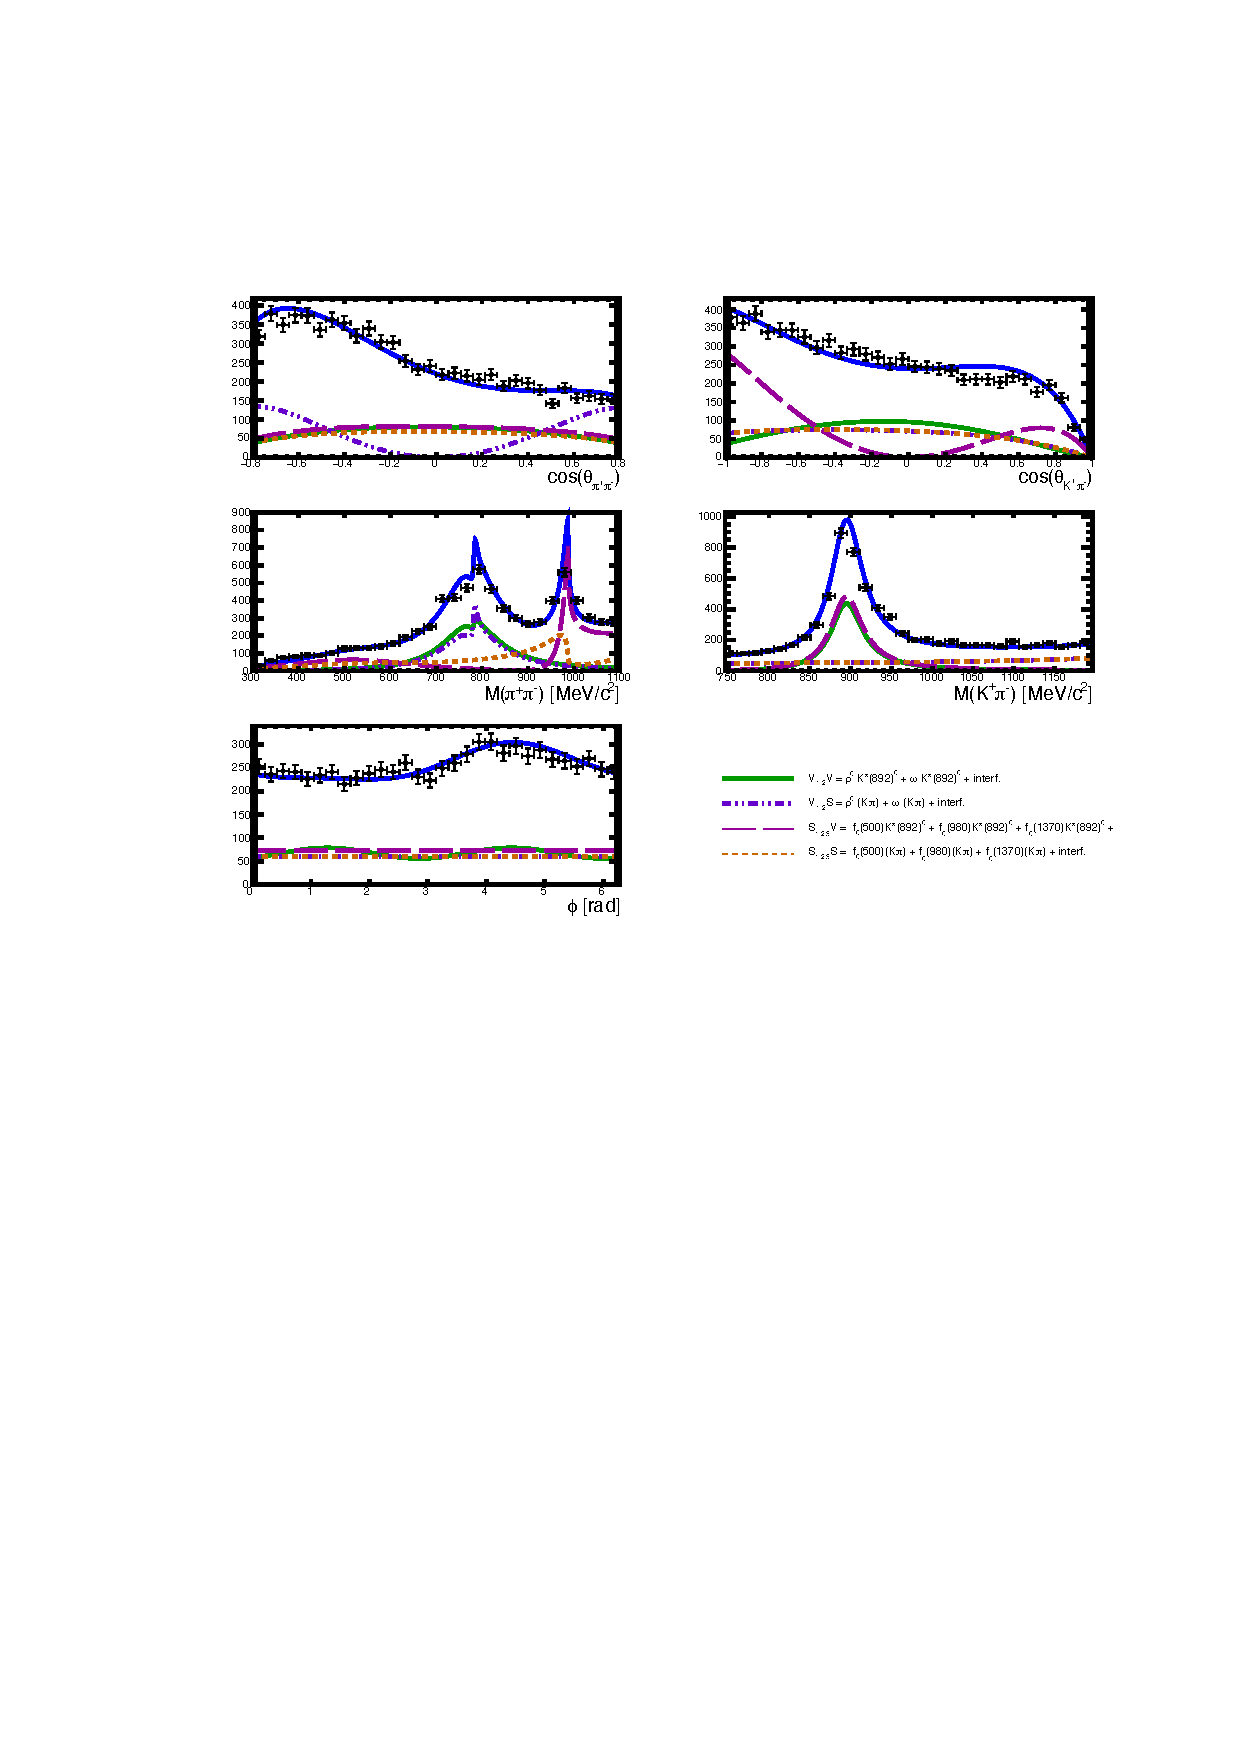
\includegraphics[width=.75\textwidth]{FiveBodyFitResults.pdf}
  \begin{itemize}
  \item All CPV observables still blind
  \item Analysis in WG review.
  \end{itemize}
\end{frame}

\begin{frame}
  \begin{block}{}
    \centering \Huge Search for the decay  \LbpkEtapr
  \end{block}
  \centering \href{https://lhcb-wg.web.cern.ch/lhcb-WG/bnoc/listentry.py?name=2011\%2B12+Lb+-\%3E+p+K+eta\%28\%27\%29+BFs\&cat=analysis}{\textcolor{blue}{Link to WG database}}
\end{frame}

\begin{frame}{Motivation}
  \begin{itemize}
  \item \etapr still not fully understood - size of gluon component in meson wavefunction?
    \begin{equation}
      \ket{\etapr} \approx \cos{\phi_{g}}\sin{\phi_{p}}\frac{1}{\sqrt{2}}\ket{\uubar + \ddbar} + \cos{\phi_{g}}\cos{\phi_{p}}\ket{\ssbar}+sin{\phi_g}\ket{gg}
    \end{equation}
    Latest measurement by \lhcb:  $\phi_{g}=(0\pm 24.6)\degrees$ (arXiv:1411.0943),  $\phi_{p} = (43.5^{+1.4}_{-1.3}) \degrees$.
  \item The decay of a \bquark baryon to an \etaorpr final state has never been observed, completely unexplored area of charmless B physics.
  \item $3\sigma$ evidence seen for \LbEtaL at \lhcb, $\mathcal{B}  = 9.3^{+7.3}_{-5.3} \times 10^{-6}$, and limit set on \LbEtapL, $\mathcal{B}<3.1 \times 10^{-6}$ (90\%) (LHCB-PAPER-2015-019).
  \end{itemize}
\end{frame}

\begin{frame}{Analysis Strategy}
  \begin{itemize}
  \item Perform blind search for \LbpkEtapr using Run I data.
  \item Reconstruct \etapr in two channels: \EtapPiPiG (BF=0.291) and \EtapPiPiEta (\EtaGG) (BF=0.169)
  \item \BpKetapr (\EtapPiPiG) used as a control channel for both rare channels.
    \begin{block}{Ratio of branching fractions extracted as:}
      \begin{equation*}
        \frac{\mathcal{B}(\Lb)}{\mathcal{B}(\Bp)} = \big(\frac{\epsilon_CN_\gamma}{\epsilon_\gamma N_C} + \frac{\epsilon_C N_\eta}{\epsilon_\eta N_C}\big)\frac{\mathcal{B}(\EtapPiPiG)}{\mathcal{B}(\EtapPiPiEta) + \mathcal{B}(\EtapPiPiG)} \frac{f_u}{f_\Lambda}
      \end{equation*}
    \end{block}
  \item $N_C (\epsilon_C)$,$N_{\gamma} (\epsilon_{\gamma})$ and $ N_{\eta} (\epsilon_{\eta})$ are yields (efficiencies) in control, \EtapPiPiG and \EtapPiPiEta channels respecitvely.
  \item Fit all channels simultaneously and extract ratio of branching fractions directly from fit.
  \end{itemize}
\end{frame}

\begin{frame}{Selection}
  \small
  \begin{itemize}
  \item Train seperate BDTs for each rare channel and optimise for Punzi FoM with $\sigma=5$.
    \begin{center}
      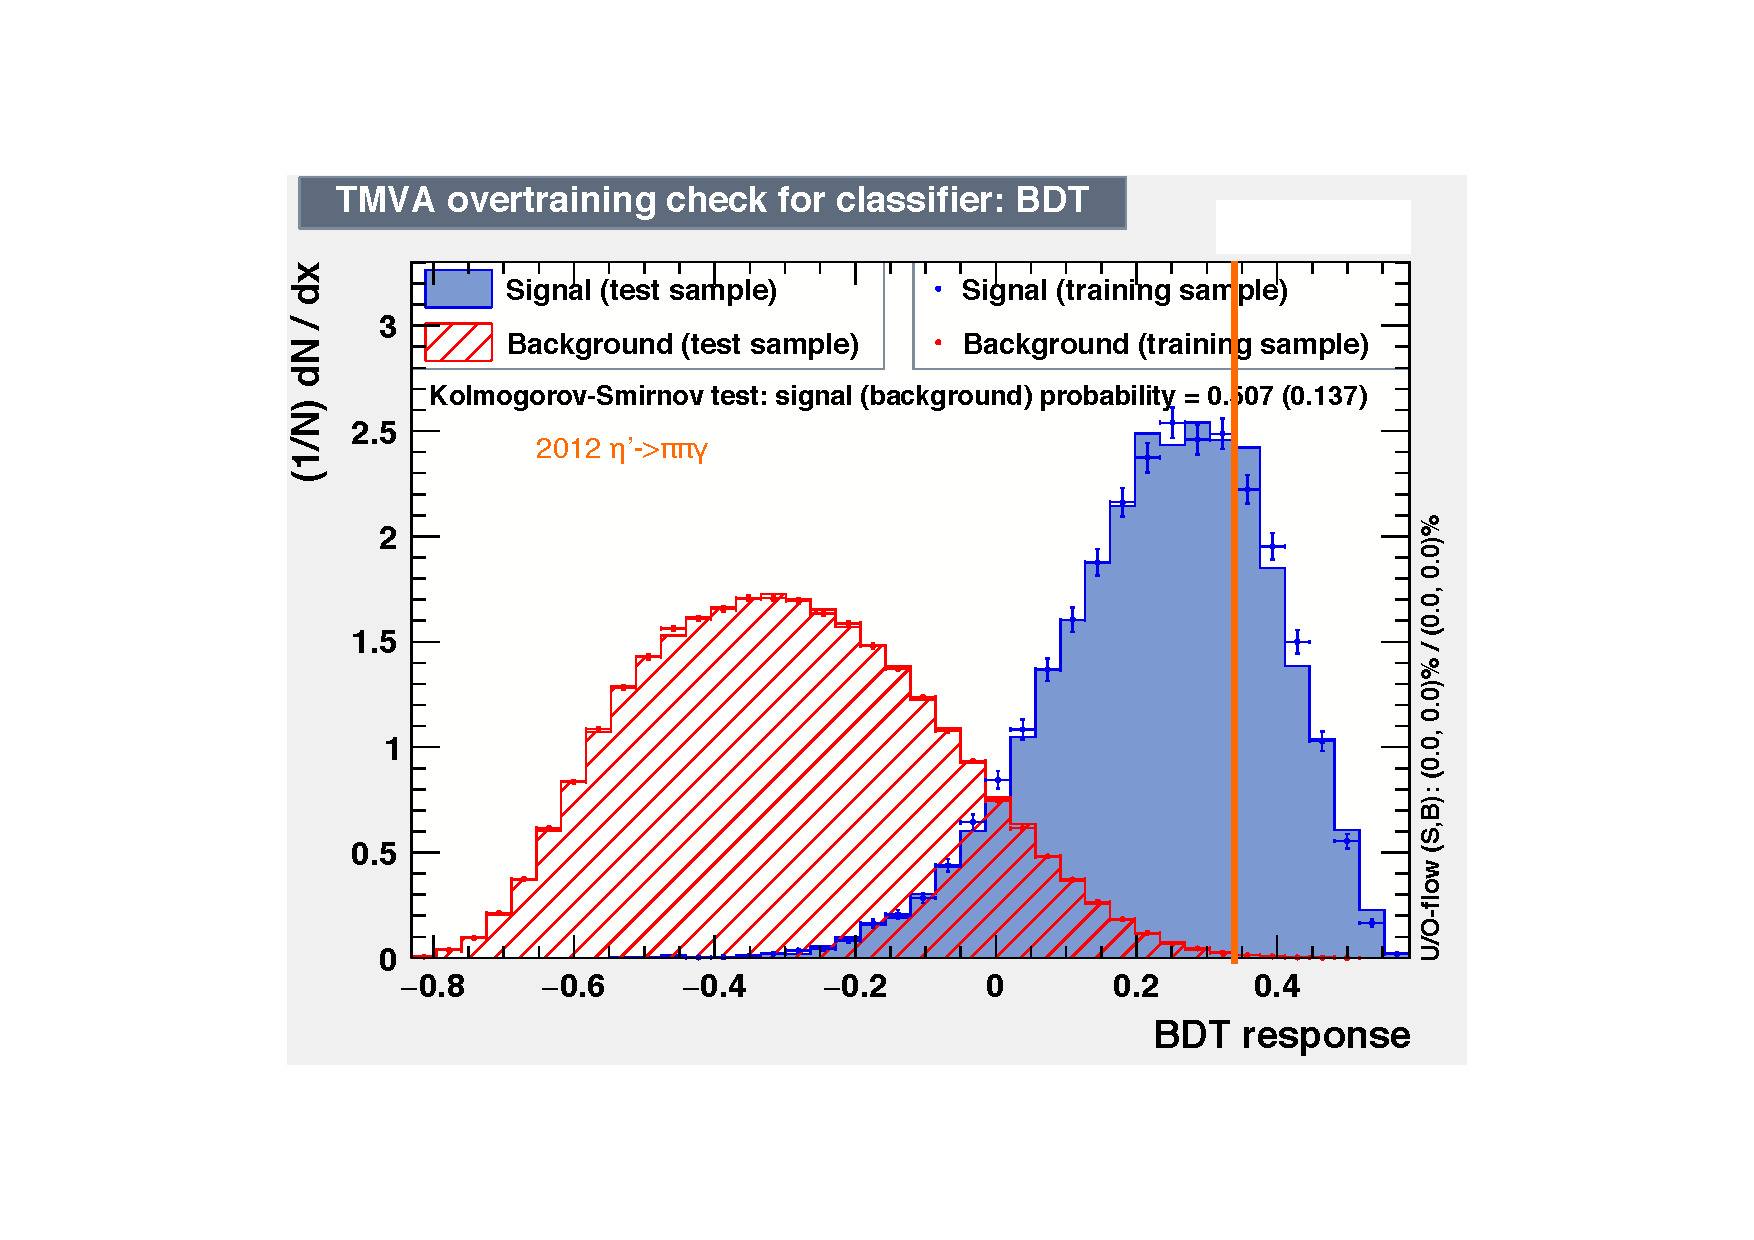
\includegraphics[width=.41\textwidth]{2012IOPpipig.pdf}
      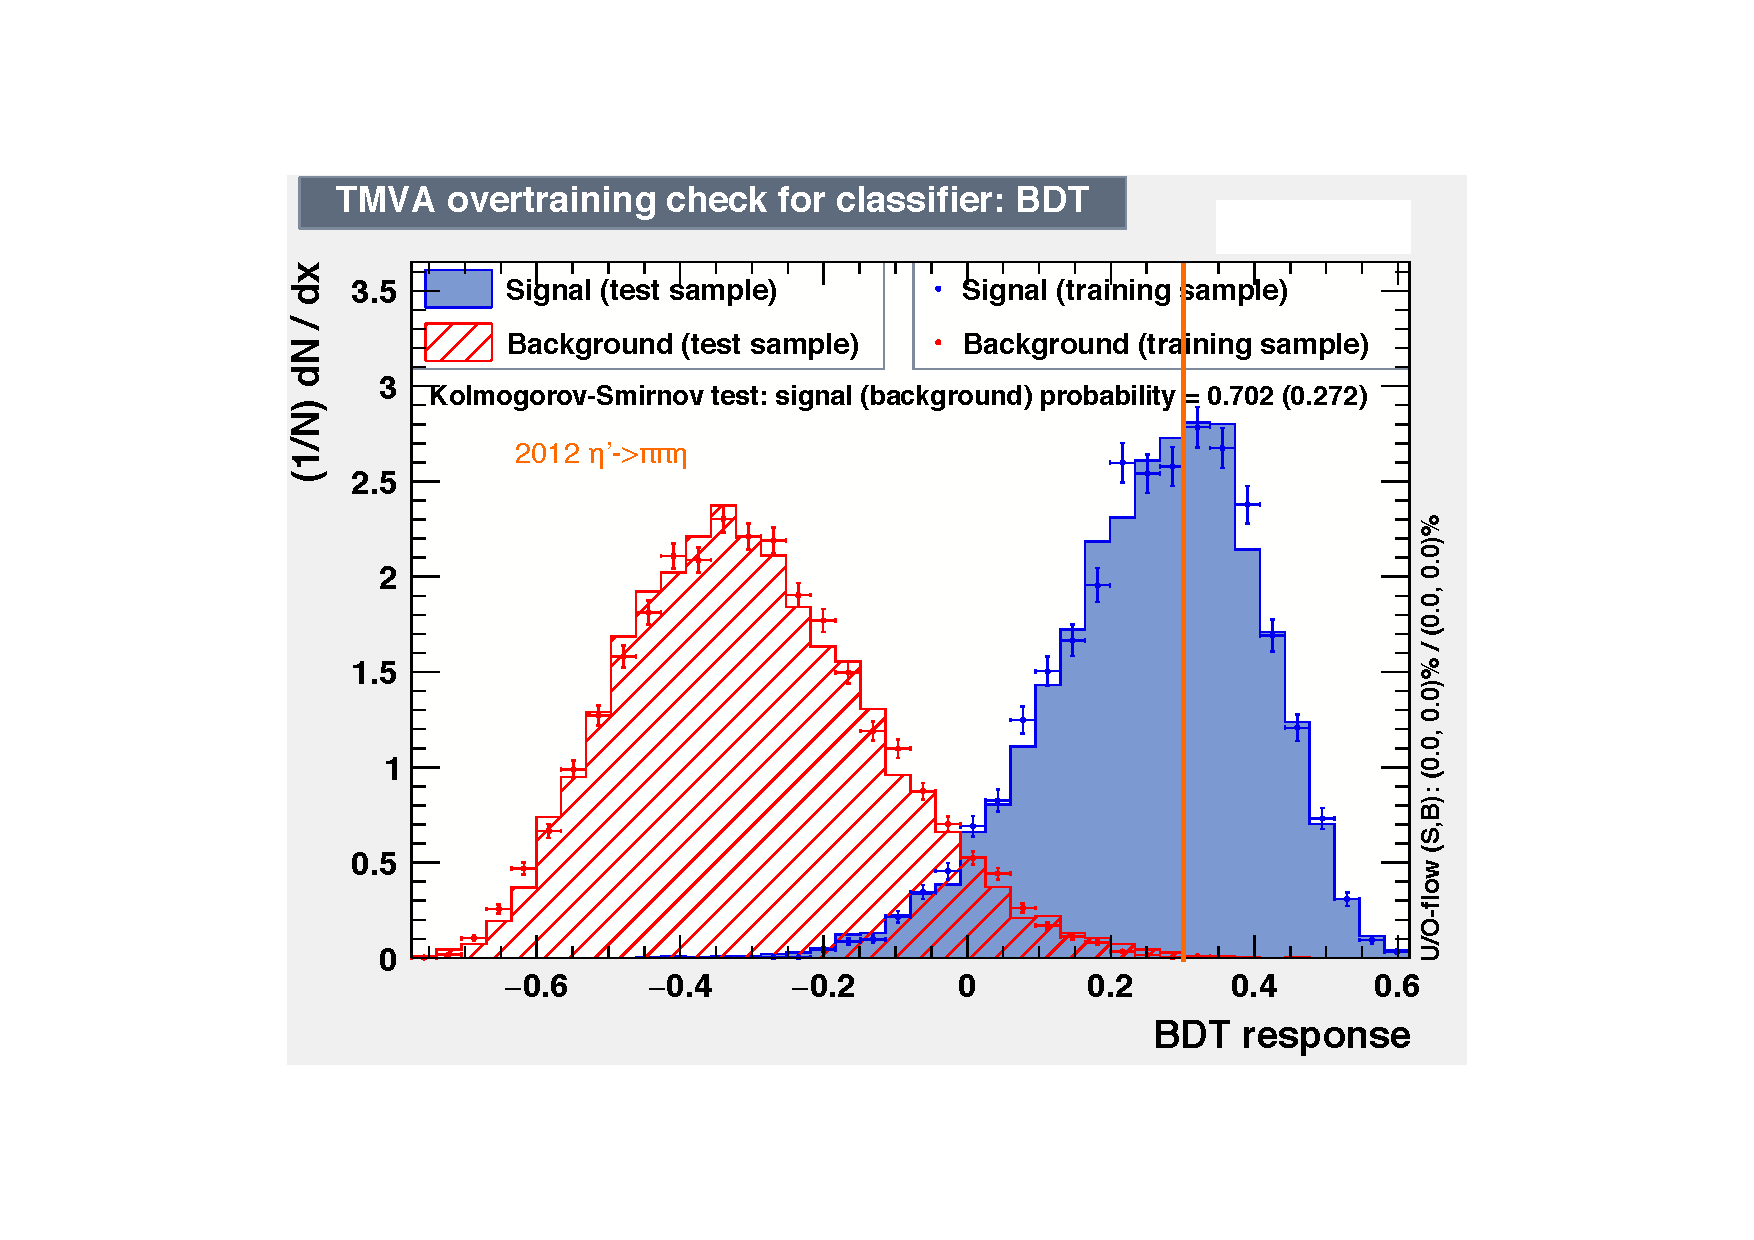
\includegraphics[width=.41\textwidth]{pipieta12IOP.pdf}
    \end{center}
  \item Similar BDT used for normalisation channel but optimised for signal significance.
  \item 3D PID optimisation performed, results in tight cuts on \texttt{ProbNN} PID variables for Proton and Kaon, looser cuts for Pions.
  \item Specific mass vetoes for charm resonances and \decay{\Lb}{\proton \Km \pip \pim} decays.
%  \item Require M(\pip \pim)\textgreater 510.0\mev in \EtapPiPiG channel to remove low mass background
%  \item Require $480.0\mev < M(\etaz)_{DTF}< 620.0 \mev$ in \EtapPiPiEta channel.

  \end{itemize}
\end{frame}

\begin{frame}{Efficiency Calculation Procedure}
\begin{itemize}
\item Rich resonant structure expected in M(\proton \Km) spectrum but not a priori known.
  \begin{columns}
    \column{.49\textwidth}
    \begin{block}{if Significance \textgreater $5\sigma$}
      \begin{itemize}
      \item Bin efficiency in square Dalitz plot (SDP) variables m' and $\theta'$.
      \item Extract sWeights from mass fit - background subtraction.
      \item Efficiency taken as:
        \begin{equation}
          \epsilon = \frac{\sum_i^{N}W_i}{\sum_i^{N}\frac{W_i}{\epsilon_i}}
        \end{equation}
        where $\epsilon_i$ is efficiency in the bin of SDP occupied by event i.
      \end{itemize}
    \end{block}
    \column{.49\textwidth}
    \begin{itemize}
    \item Need to take into account efficiency variation over phase space of \LbpkEtapr decay.
    \end{itemize}
    \begin{block}{if Significance \textless $5\sigma$}
      \begin{itemize}
      \item Fill 1D histogram of efficiency for each bin of SDP.
      \item Use mean value for efficiency and assign RMS as systematic uncertainty.
      \end{itemize}
    \end{block}
  \end{columns}
\end{itemize}
\end{frame}

\begin{frame}{Signal Channel Mass Fits}
  \begin{itemize}
  \item All signal shapes modelled with DCB
  \item Combinatorial background modelled with exponential (2nd order polynomial) in rare (control) channel.
  \item \EtapPiPiG channel also suffers from \decay{\Lb}{4h + \piz} background, modelled with bifurcated Gaussian - shape fixed to MC.
  \end{itemize}
  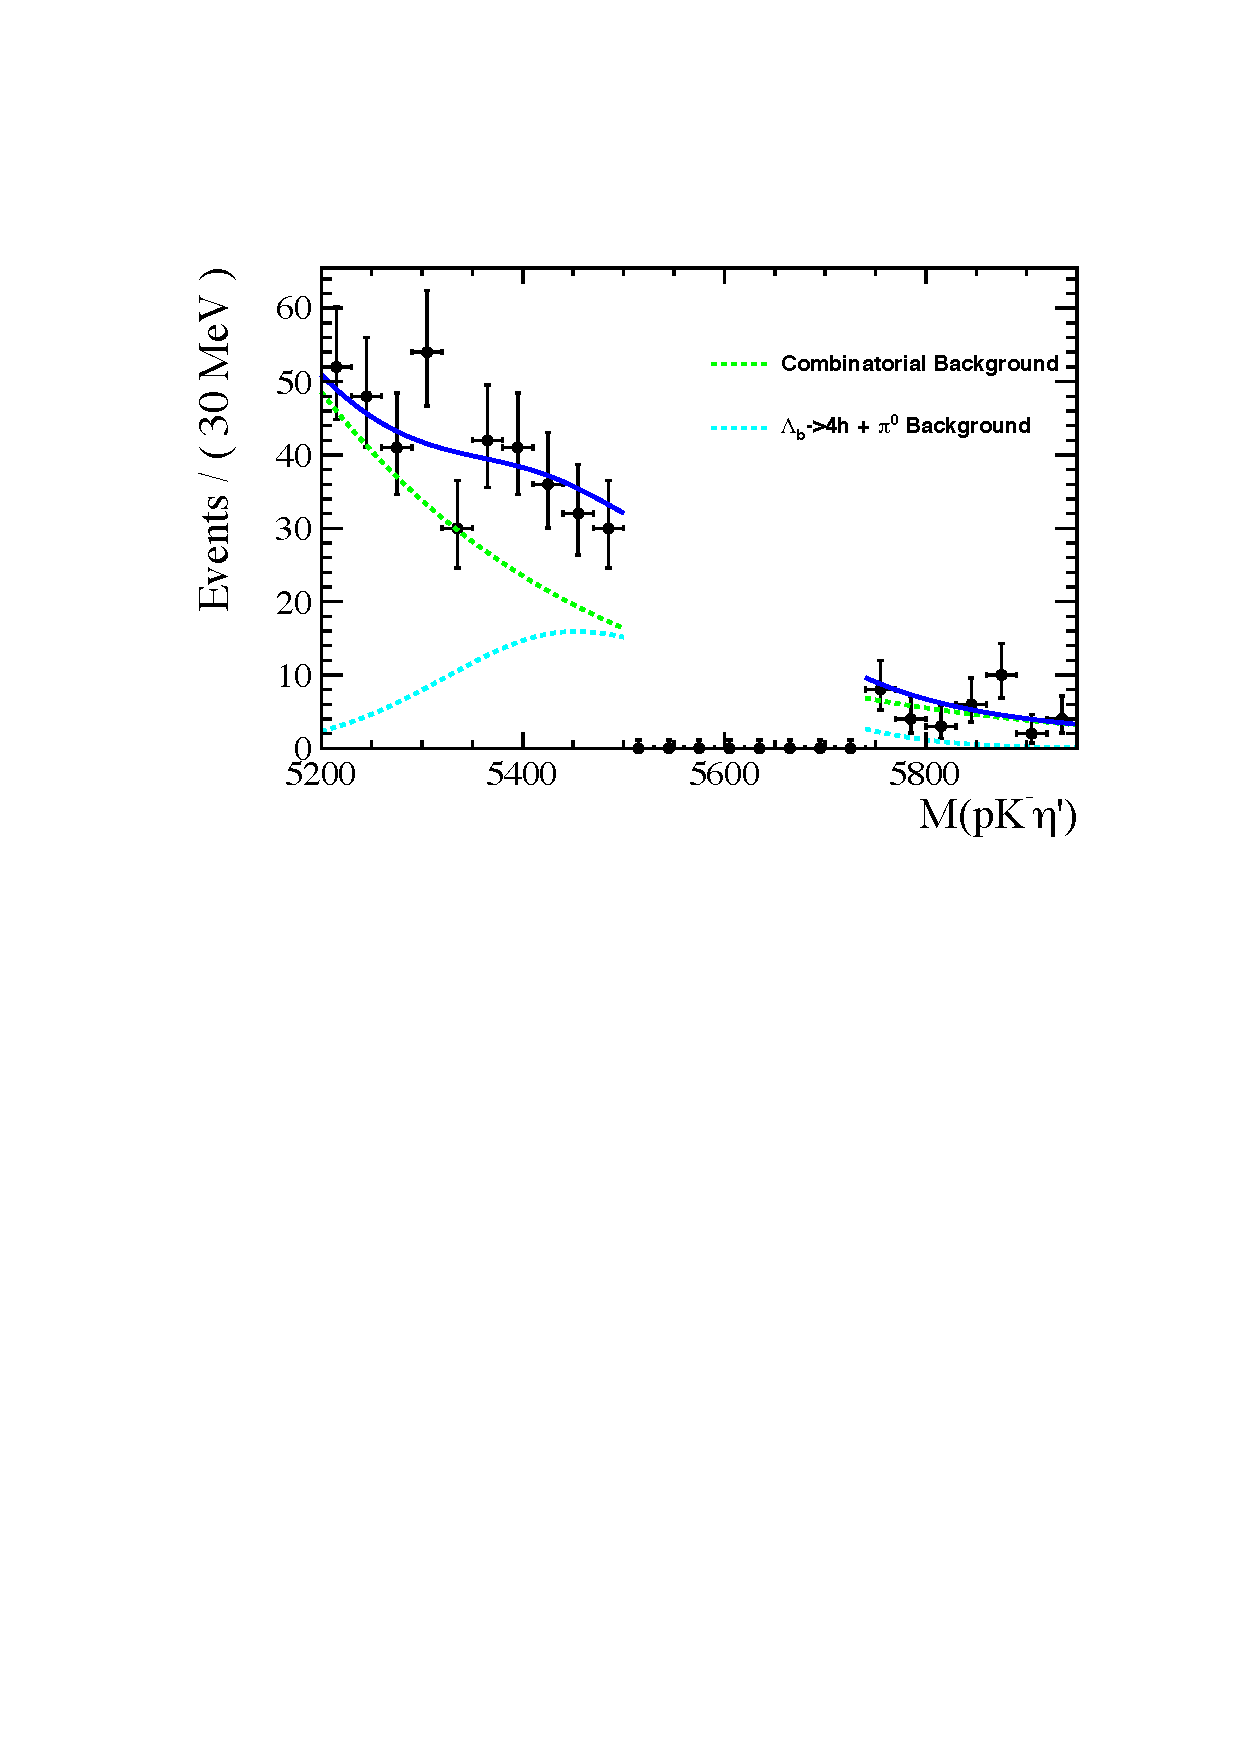
\includegraphics[width=.49\textwidth]{PiPiGFit.pdf} 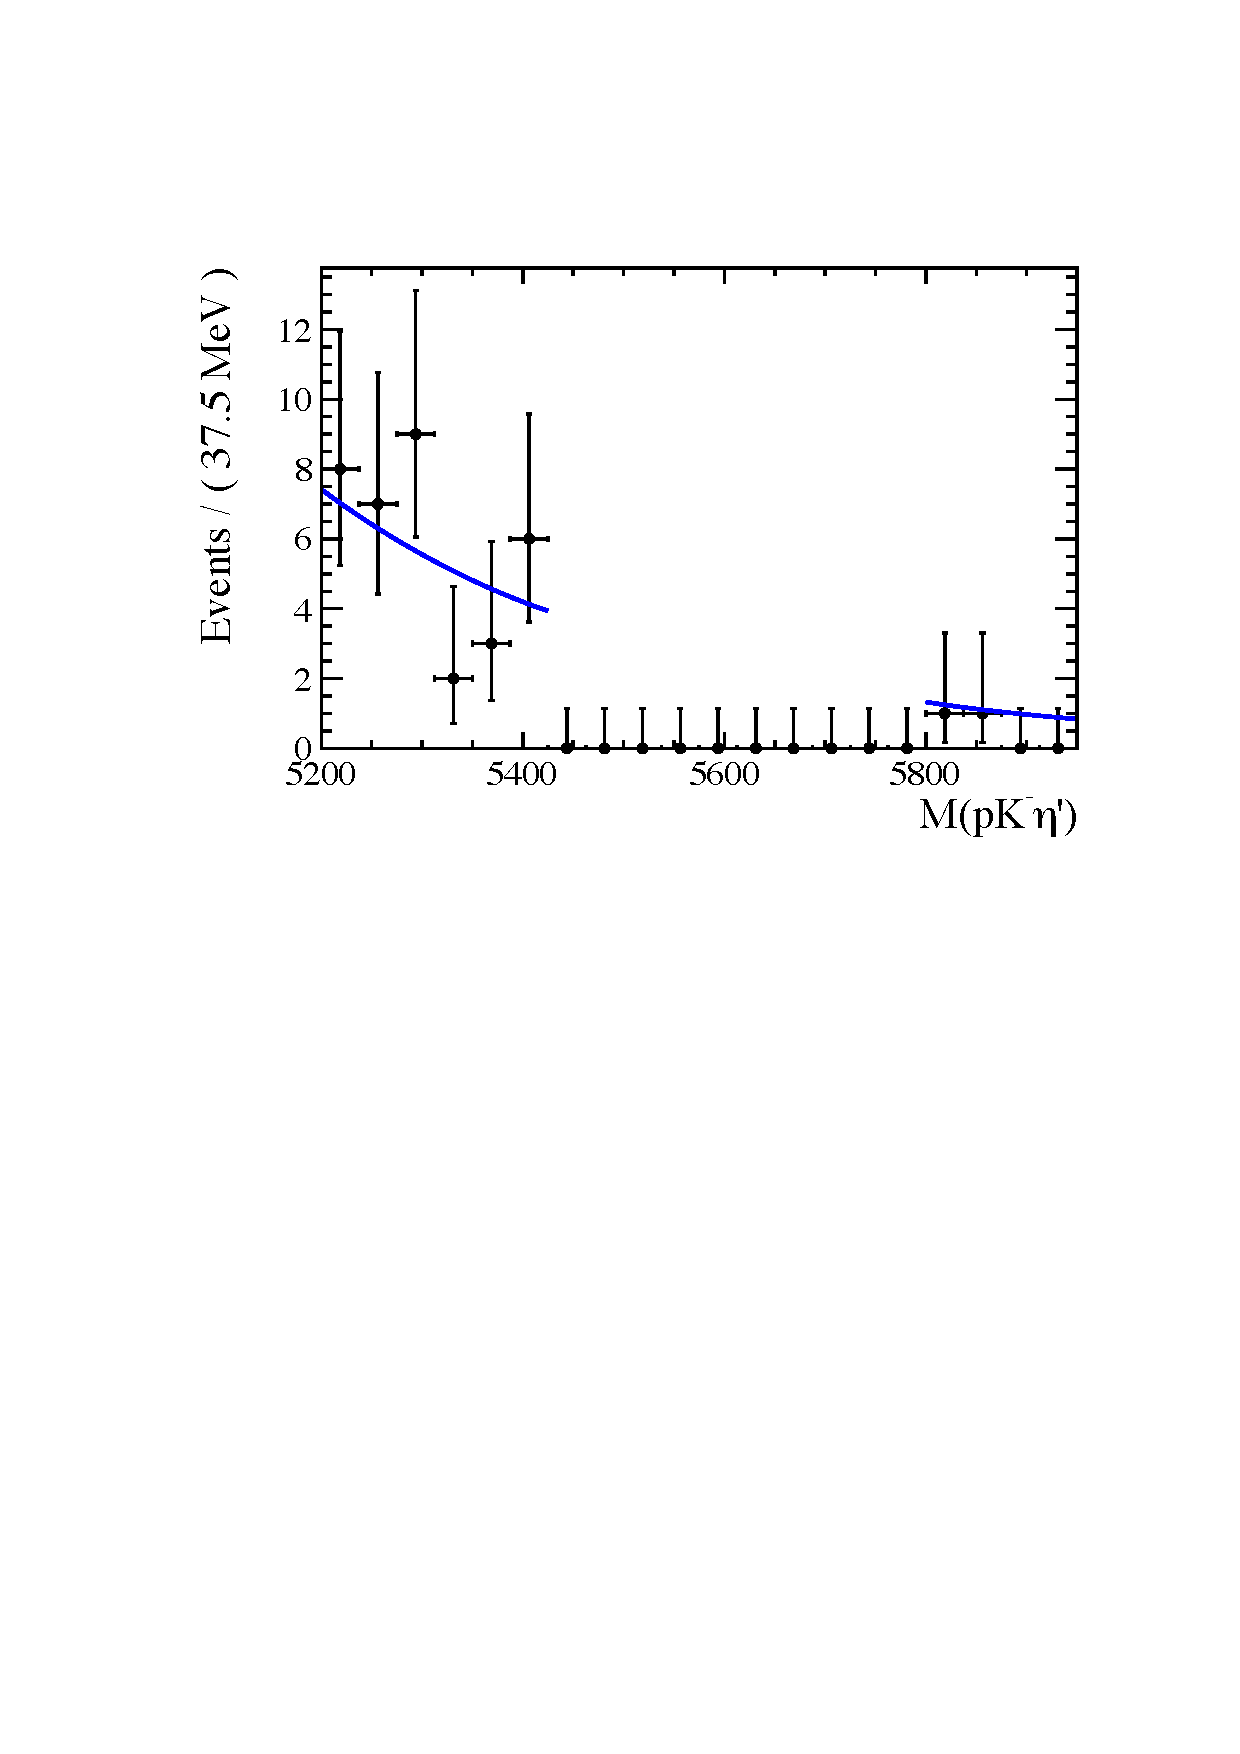
\includegraphics[width=.49\textwidth]{PiPiEta.pdf}
\end{frame}

\begin{frame}{Expected Sensitivity and Outlook}
  \begin{itemize}
  \item Toy studies have been performed for a range of \BF \xspace assumptions - statistical significance caluclated with Wilk's theorem.
    \begin{center}
      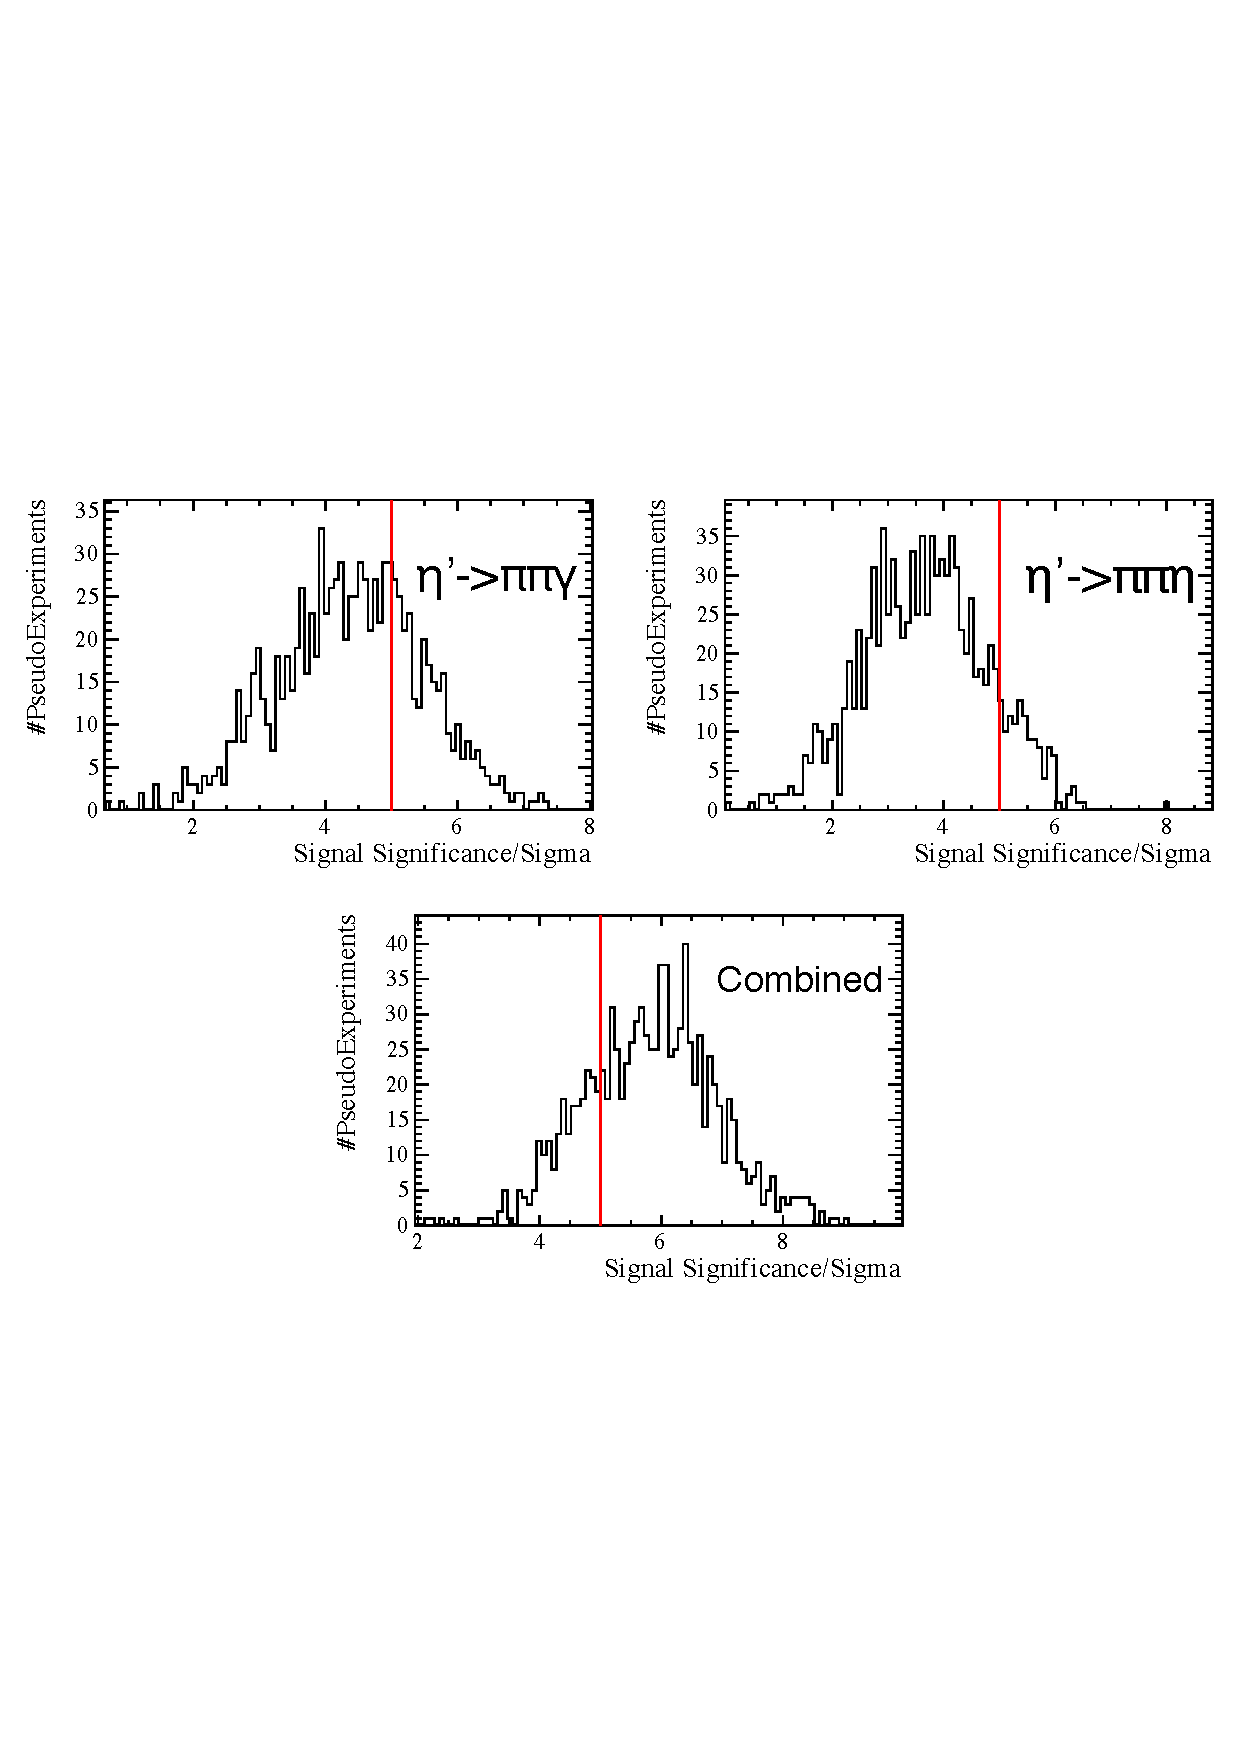
\includegraphics[width=.6\textwidth]{LbpketaprSensitivity.pdf}
    \end{center}
  \item $~77\%$ chance of $5\sigma$ observation if \BF(\LbpkEtapr)$=4\times10^{-6}$
  \item Analysis in WG review.
  \end{itemize}
\end{frame}

\begin{frame}
  \begin{block}{}
    \centering \Huge Search for CP violation in \decay{\PXi_{b}}{\proton \Kp \Km} decays.
  \end{block}
\end{frame}

\begin{frame}{Overview}
  \begin{itemize}
  \item \decay{\PXi_{b}}{\proton \Kp \Km} was observed for the first time using Run I data
  \item Next step is a search for CPV using amplitude analysis - $\geq \sim300$ events required.
    \begin{center}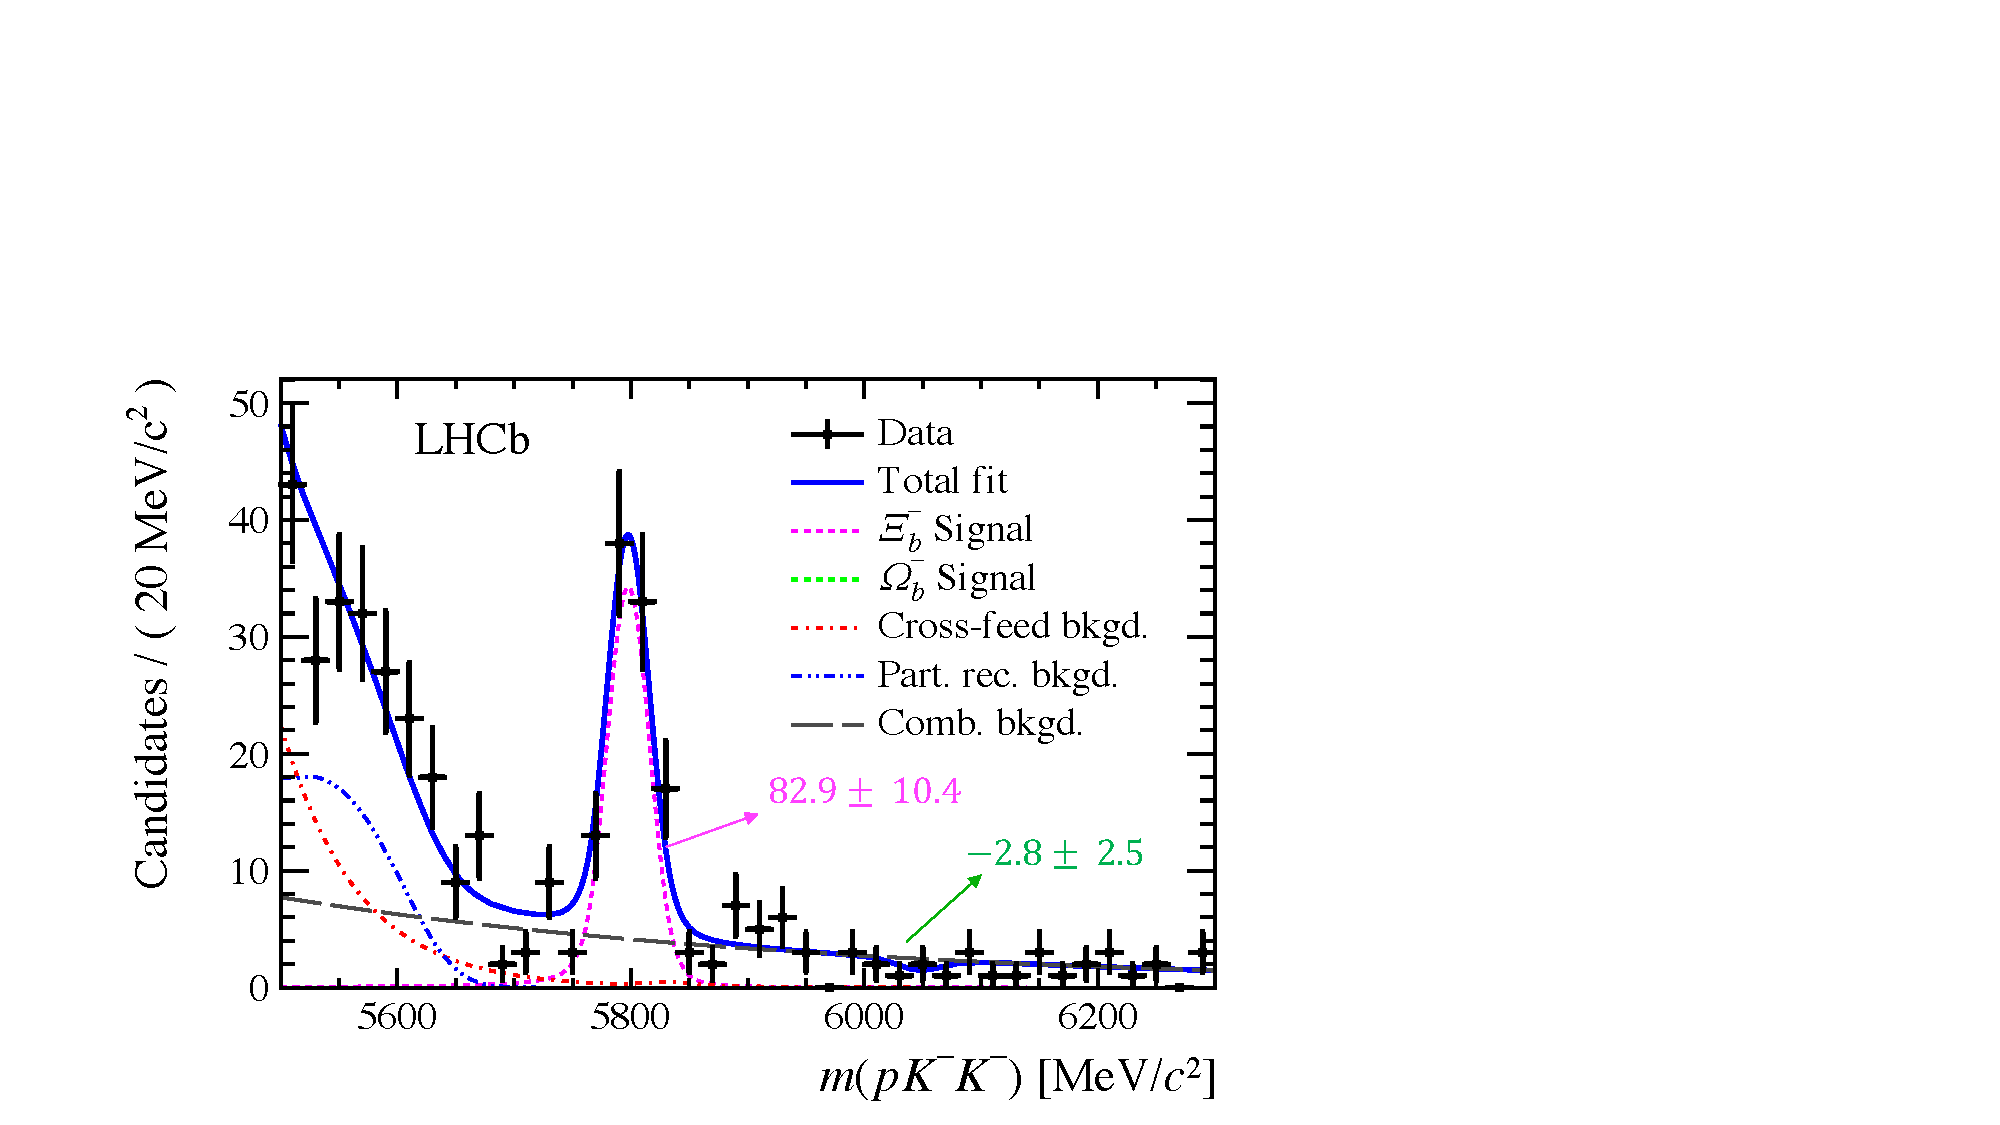
\includegraphics[width=0.6\textwidth]{XiBFit.pdf}\end{center}
  \item Plan to achieve this - Improve selection and add Run II data.
  \end{itemize}
\end{frame}

\begin{frame}{\decay{\PXi_{b}}{\proton \Kp \Km} Run I improvements}
  \small
  \begin{block}{Changes to Run I selection}
    \begin{itemize}
    \item Switch to using inclusive \texttt{Xb2phhLine} stripping line - $15\%$ improvement in stripping efficiency.
    \item Include PID in MVA, use \texttt{xGBoost} algorithm and optimise for signal significance.
    \end{itemize}
  \end{block}
  \begin{columns}
    \begin{column}{.5\textwidth}
      \begin{itemize}
      \item Very preliminary fit to Run I data shows yield of $\sim 140$ events with new selection.
      \item Should be able to observe $\geq \sim300$ signal events when Run II data is included.
      \end{itemize}
    \end{column}
    \begin{column}{.5\textwidth}
      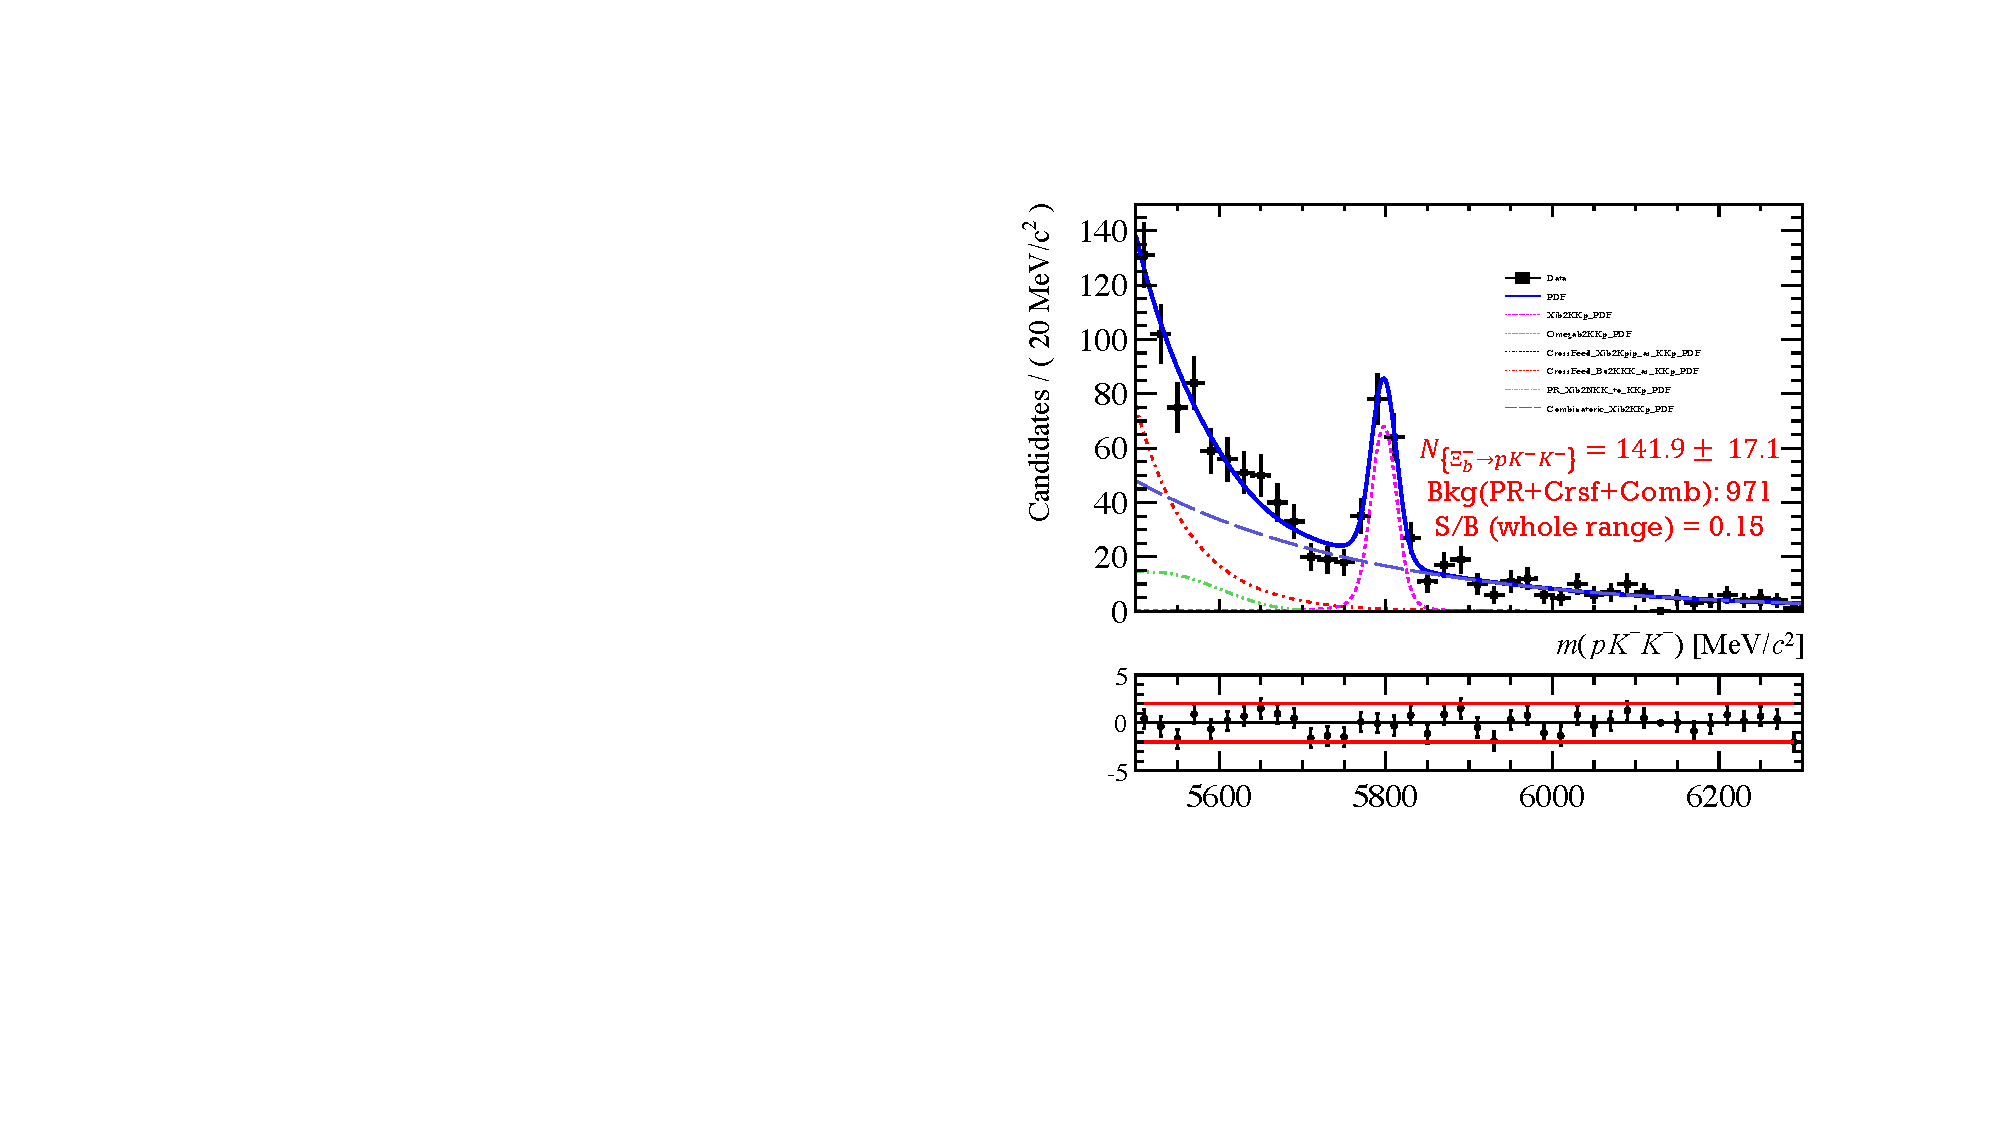
\includegraphics[width=\textwidth]{Run1ImprovedXib.pdf}
    \end{column}
  \end{columns}
\end{frame}

\begin{frame}{CPV in \decay{\Lb}{\proton h h h}}
  \begin{block}{}
    \begin{center}
      \Huge CPV in \decay{\Lb}{\proton h h h}
    \end{center}
  \end{block}
\end{frame}

\begin{frame}{Current Status}
  \small
  \begin{columns}
    \begin{column}{.4\textwidth}
      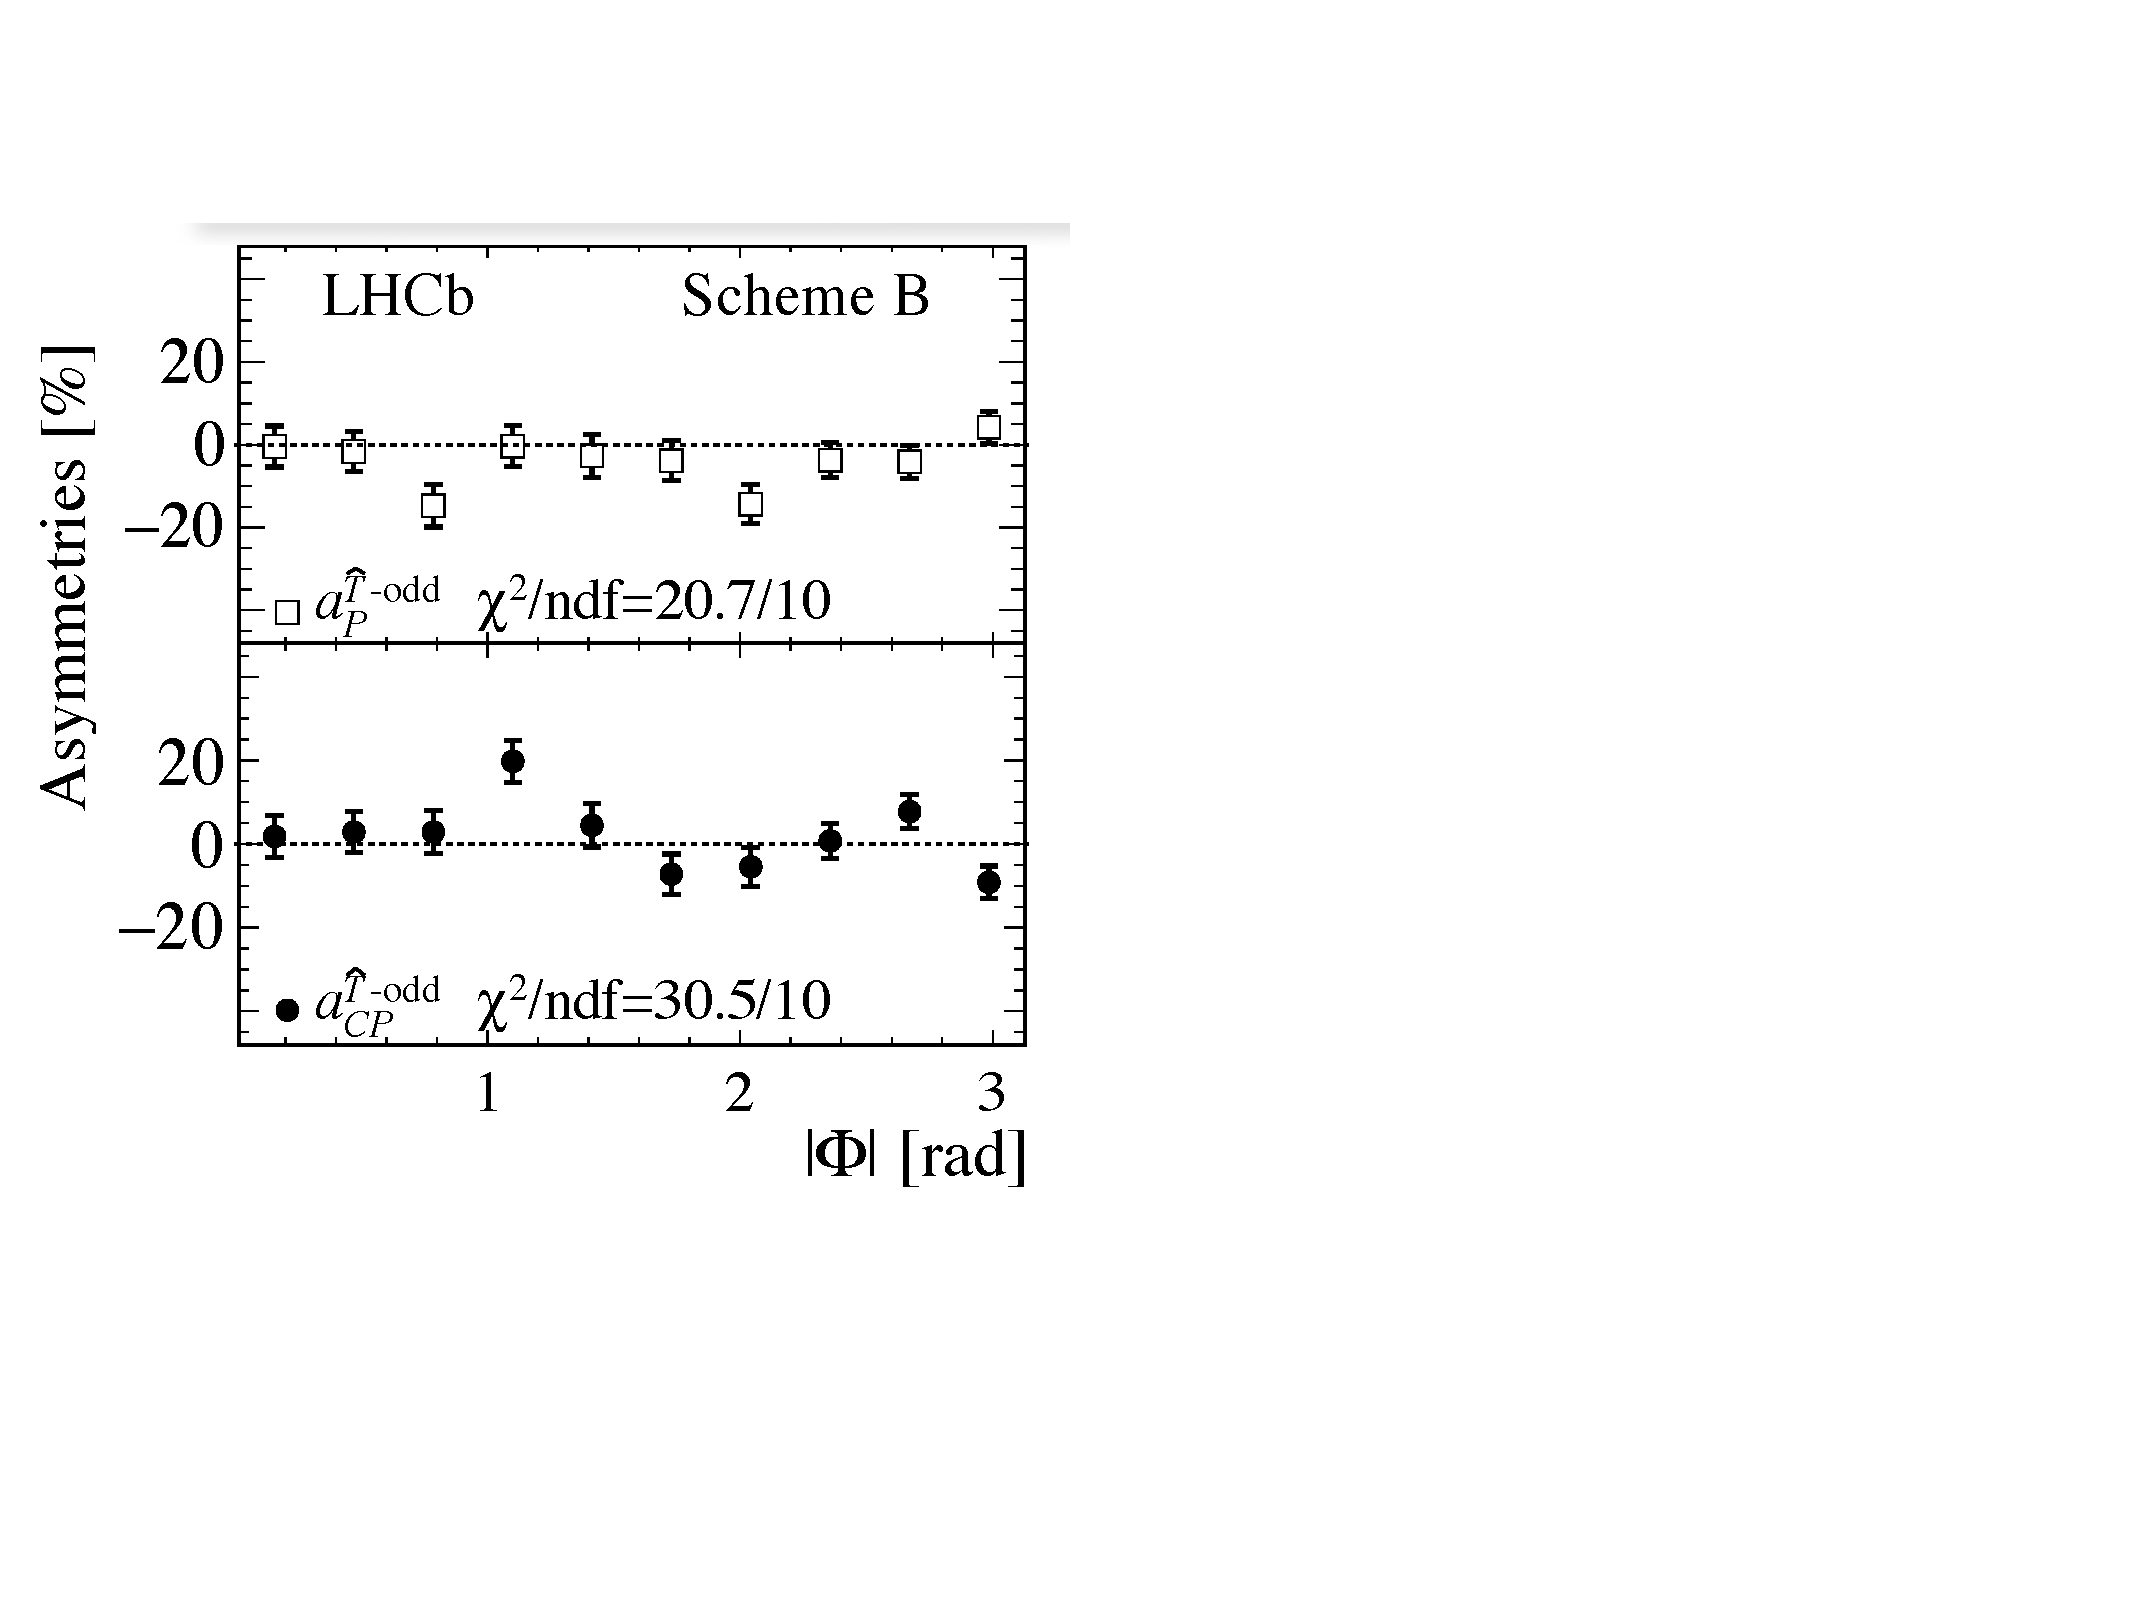
\includegraphics[width=\textwidth]{Run1CPV.pdf}
    \end{column}
    \begin{column}{.65\textwidth}
      \begin{itemize}
      \item Using Run I data $3.3\sigma$ evidence for CPV in \decay{\Lb}{\proton \pim\pip\pim} decays was observed.
      \item Used T-odd triple product asymmsetries.
      \item First evidence for CPV in a baryon decay! \href{http://www.nature.com/nphys/journal/v13/n4/full/nphys4021.html}{\textcolor{blue}{Nature Physics 13 (2017)}}
      \item More results from other deacy modes in review comittee!
      \end{itemize}
    \end{column}
  \end{columns}
  \begin{center}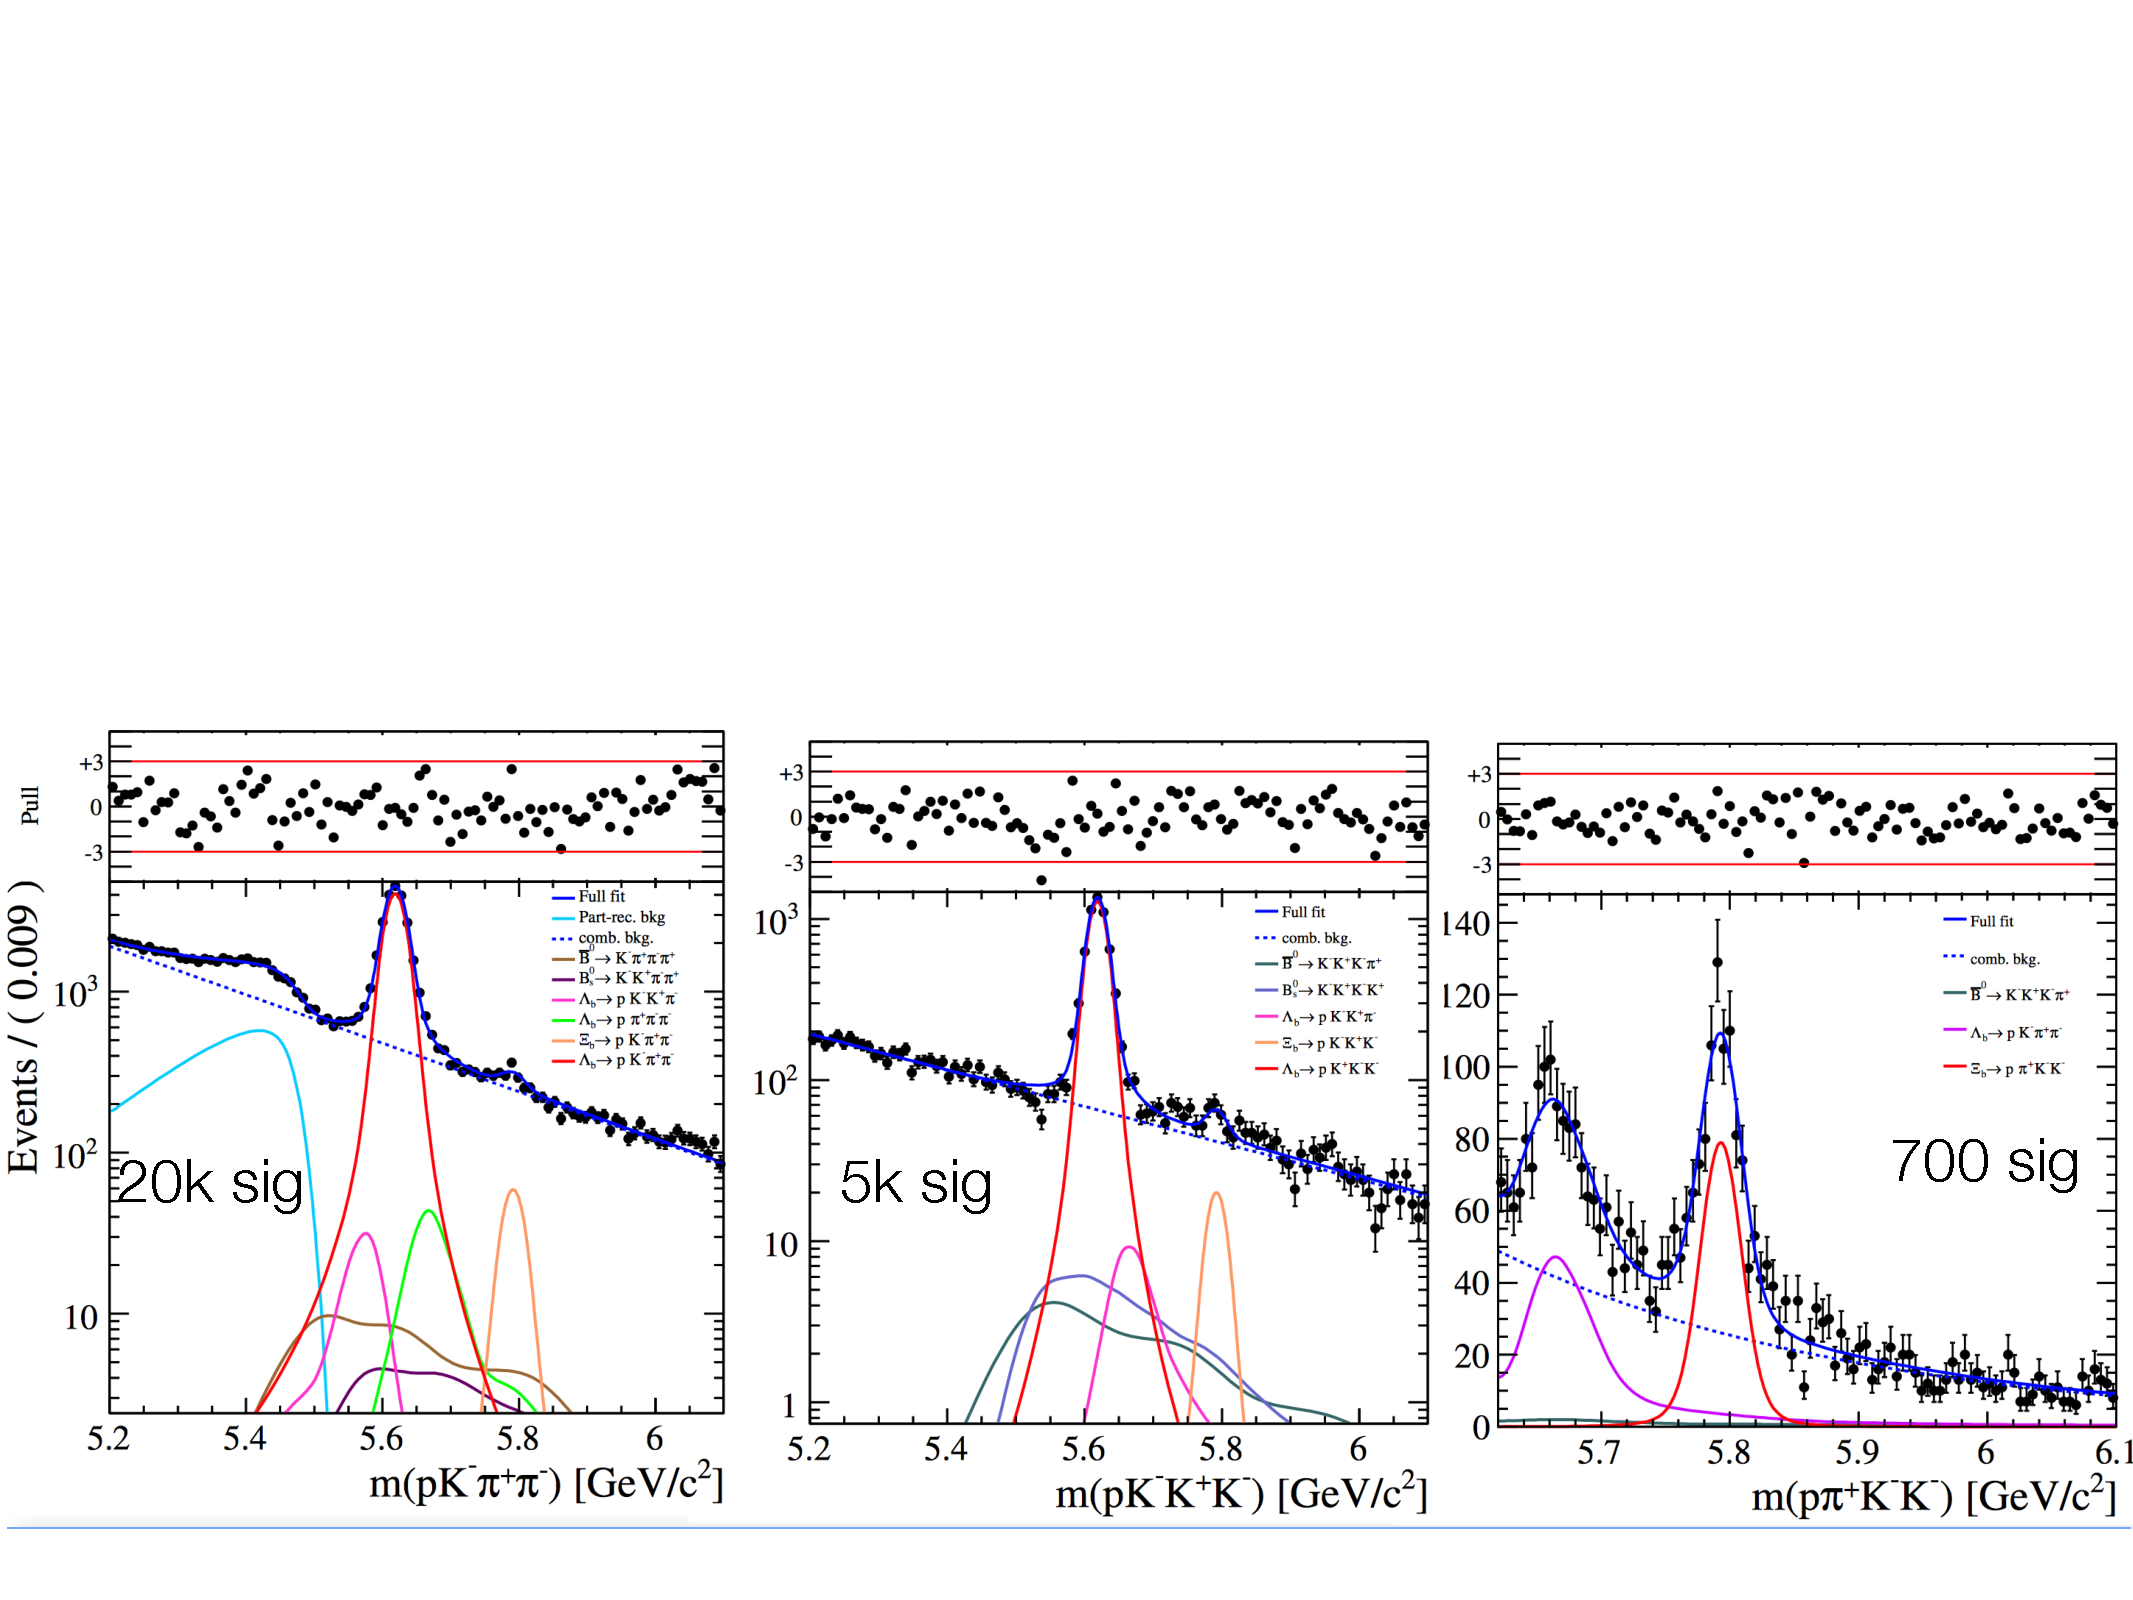
\includegraphics[width=.75\textwidth]{NewCPVChannels.pdf}\end{center}
\end{frame}

\begin{frame}{Run II Update}
  \small
  \begin{itemize}
  \item Run II update of CPV analyses planned.
  \item Expect factor $\sim3$ increase in signal yield with addition of 2016 and 2017 data
  \begin{center}
    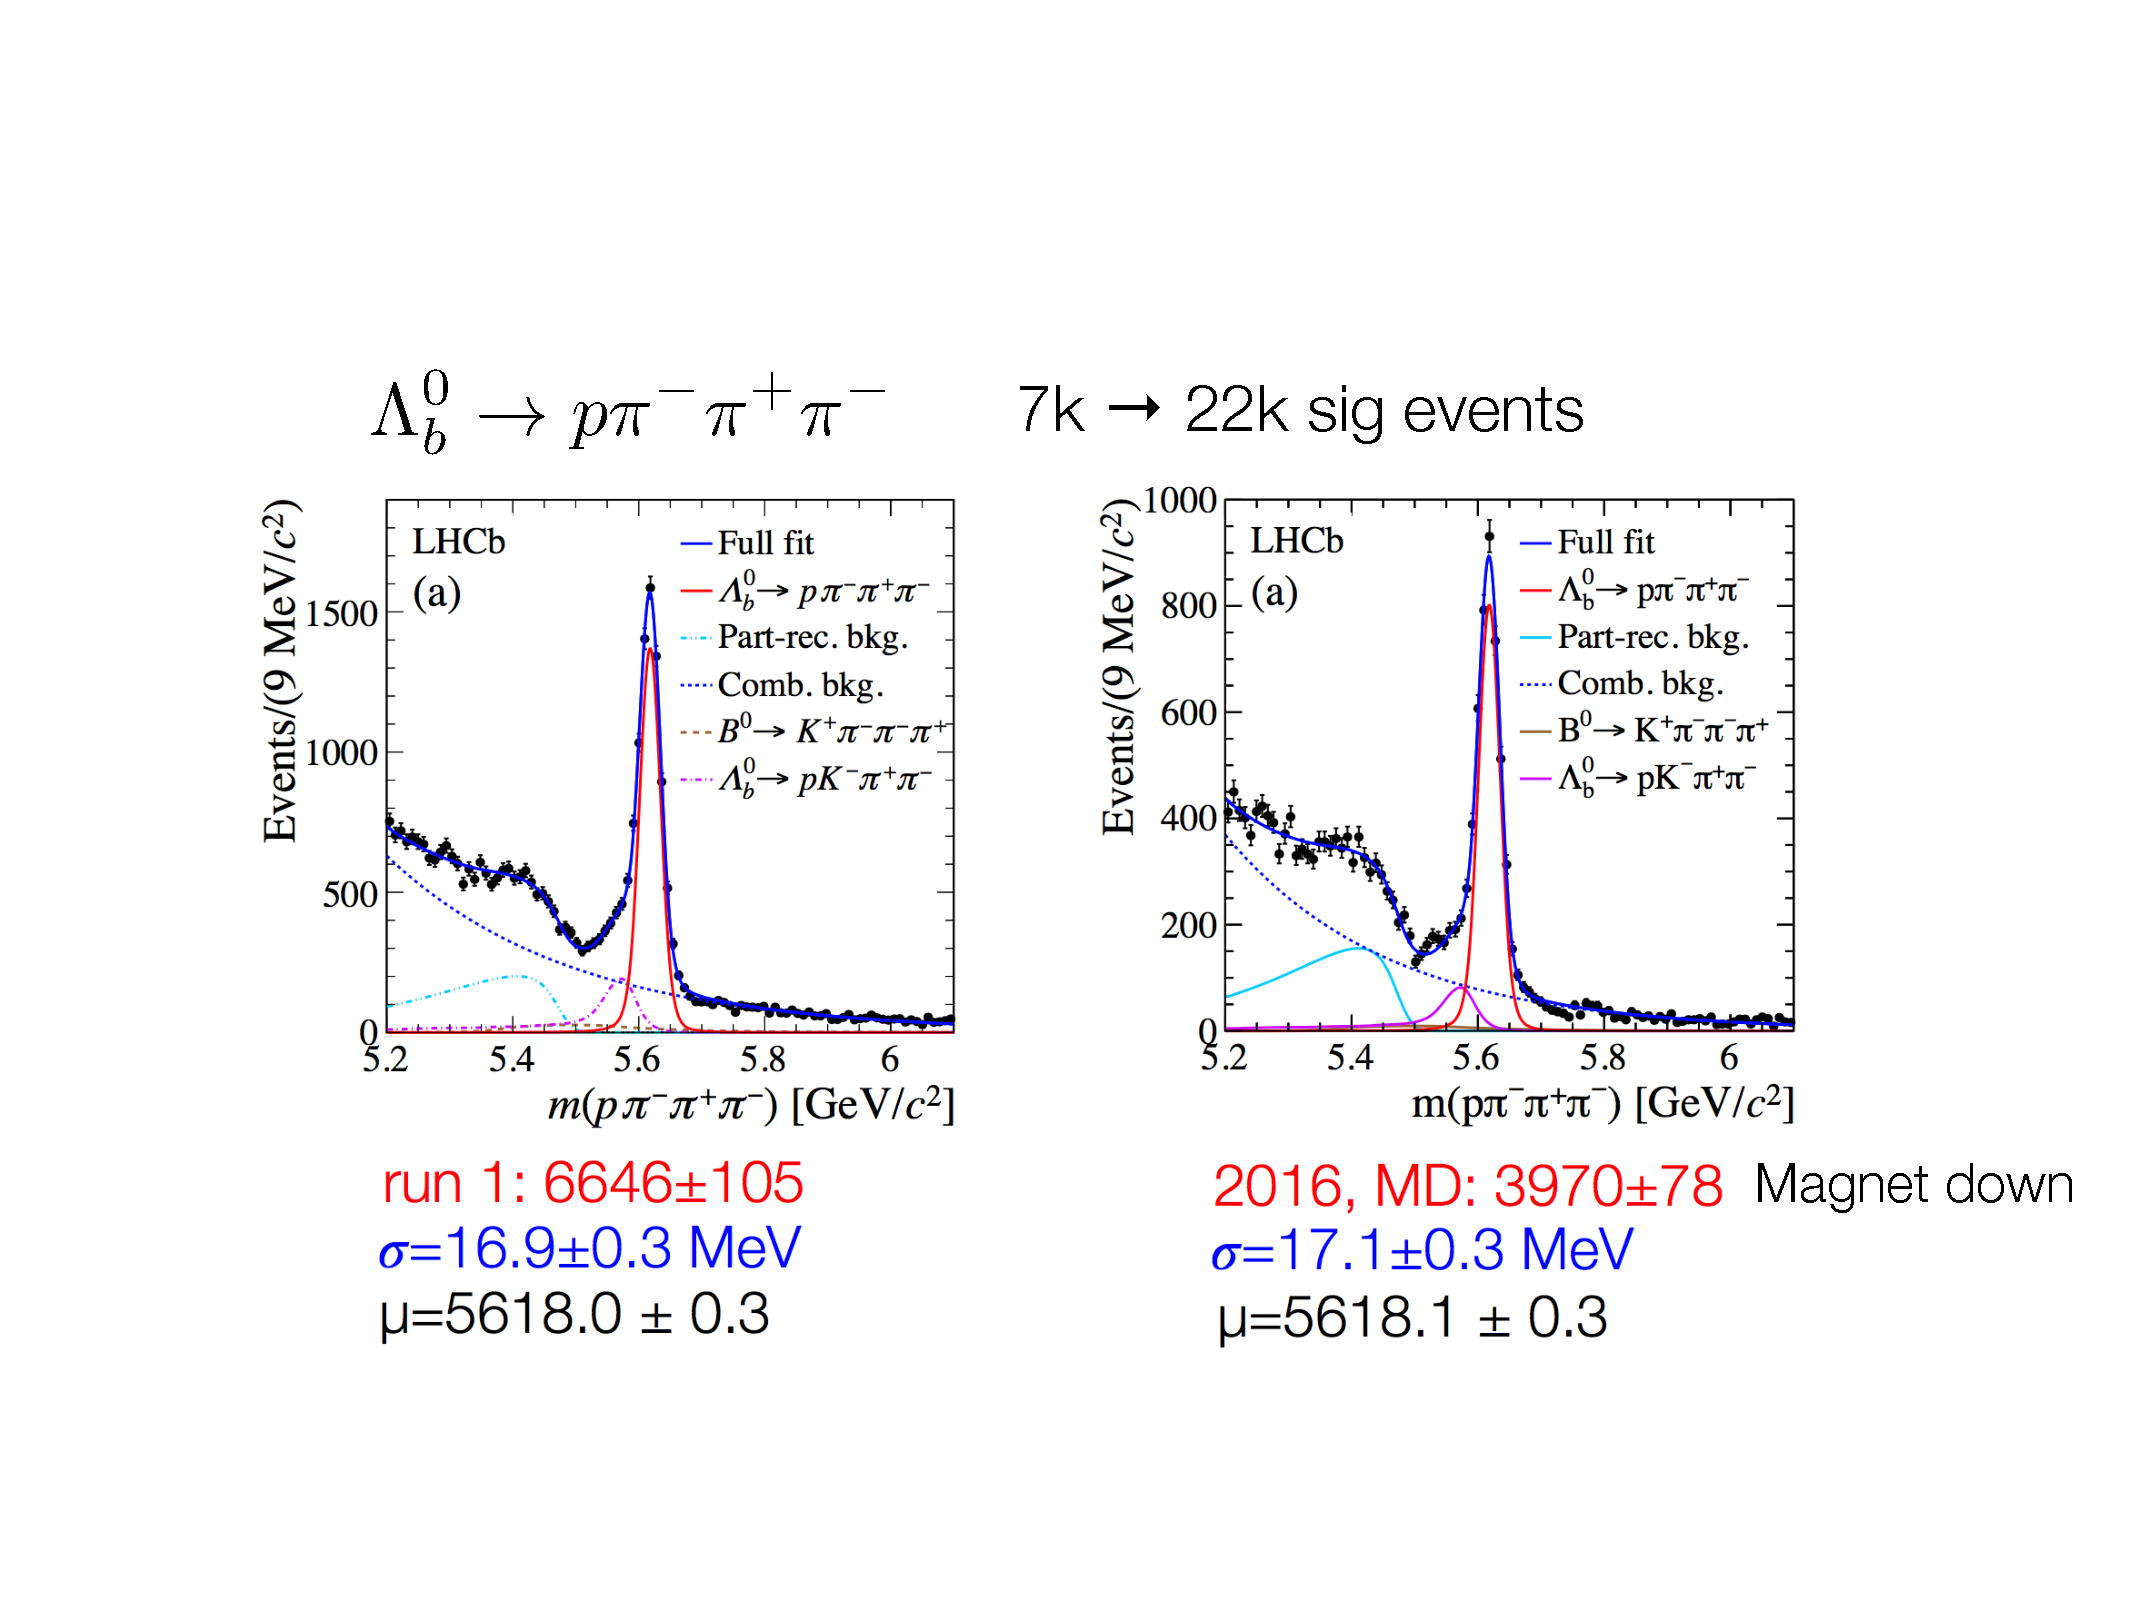
\includegraphics[width=.8\textwidth]{Run2FirstLook.pdf}
  \end{center}
  \item First look at 2016 MagDown data shows promising yield - selection not optimised and cross-feed studies needed
  \end{itemize}
\end{frame}

\begin{frame}{Energy Test}%jax2dtki
  \begin{itemize}
  \item Work under way to use energy test method to search for both P even and P odd CP violation - \href{https://arxiv.org/abs/1612.04705}{\textcolor{blue}{arxiv:1612.04705}}
  \item Define test statistic based on distances between particles and anti-particles in phase space.
  \end{itemize}
  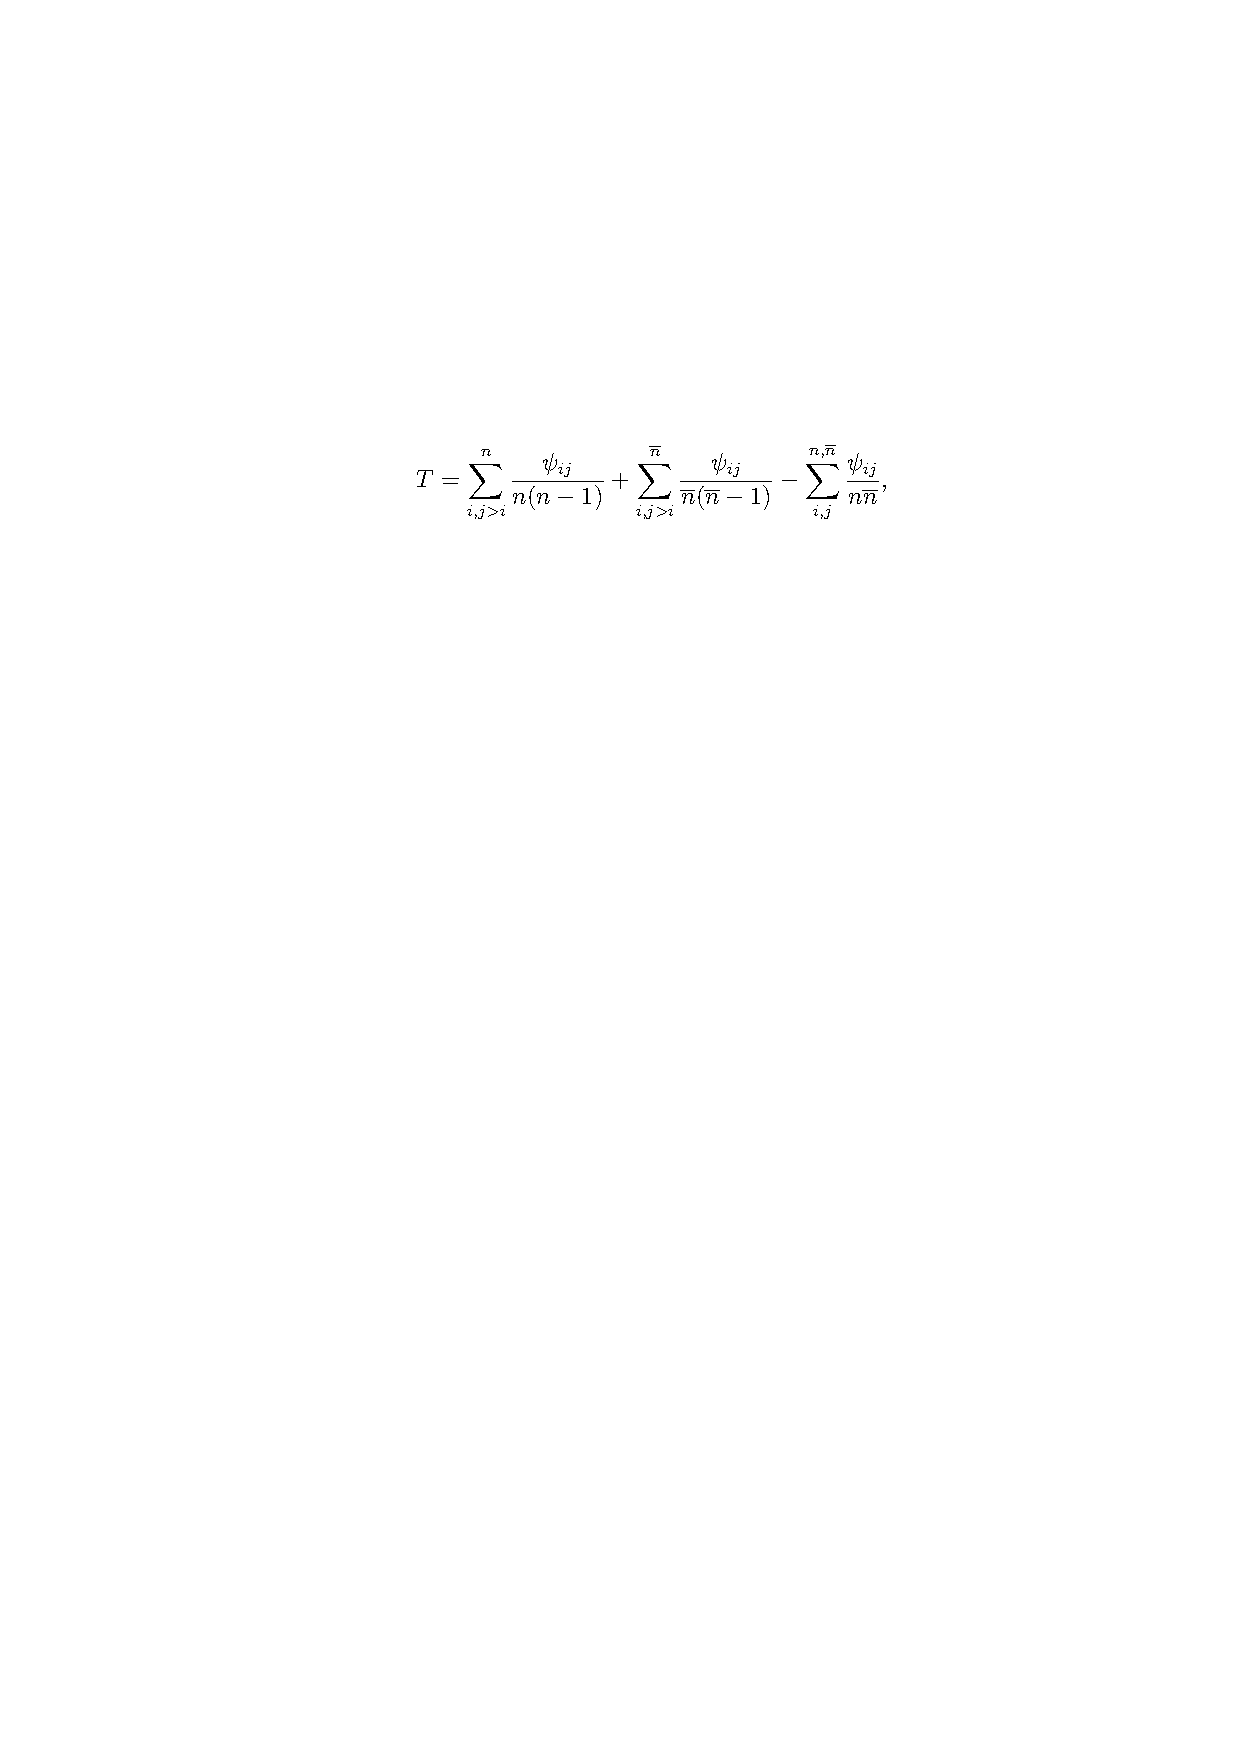
\includegraphics[width=.5\textwidth]{TestSta.pdf}\hspace{0.5cm}
\includegraphics[width=.4\textwidth]{DistanceFunc.pdf}
  \begin{columns}
    \begin{column}{.49\textwidth}
      \begin{itemize}
      \item Sensitivity studies based on RunI + 2015 +2016 data performed using cocktail of RapidSim samples, CPV artificially introduced by increasing relative fraction of $\PDelta^{+}$ events by $30\%$.
      \end{itemize}
    \end{column}
    \begin{column}{.49\textwidth}
      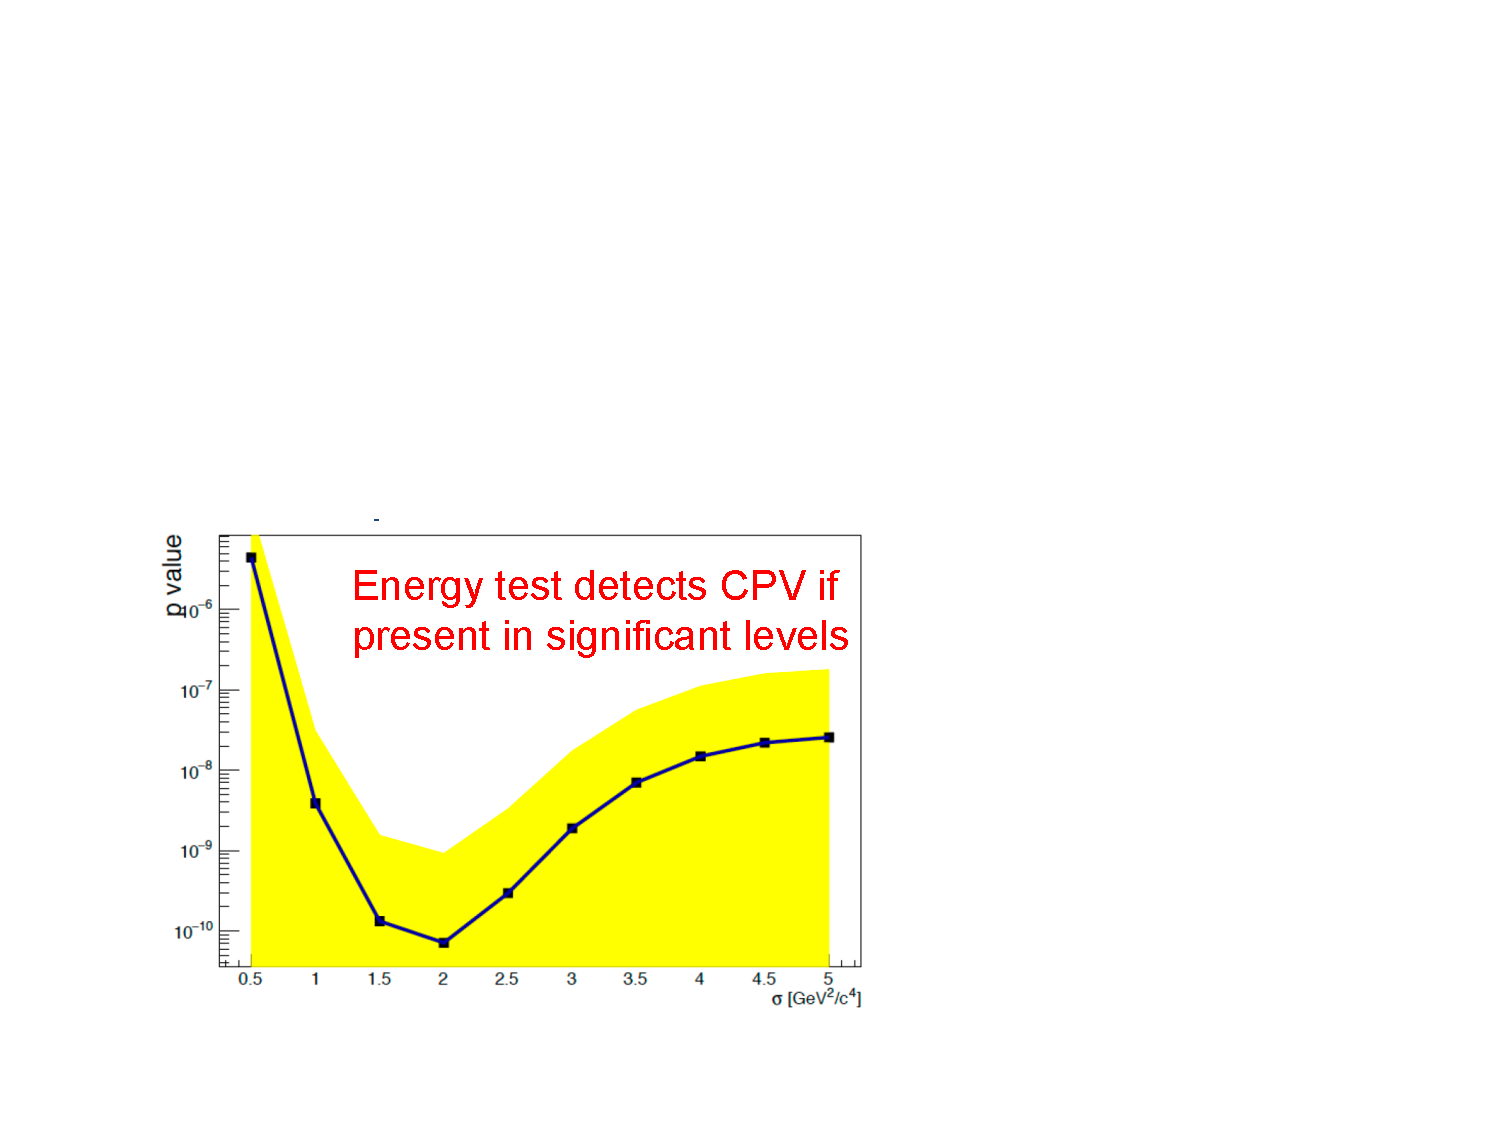
\includegraphics[width=\textwidth]{SPVSensitivity.pdf}
    \end{column}
  \end{columns}
\end{frame}

\begin{frame}{Summary of \decay{\Lb}{\proton h h h} CPV searches}
  \begin{itemize}
  \item First evidence for CP violation has been seen in \decay{\Lb}{\proton \pim \pip \pim} decays at level of $3.3\sigma$ using Run I data - Run II update planned.
  \item Run I results for \decay{\Lb}{\proton \Km \pip \pim}, \decay{\Lb}{\proton \Km \Kp \Km} and \decay{\Lb}{\proton \pip \Km \Km} decays still blind and in review comittee
  \item Work started on using energy test method to search for CP violation in \decay{\Lb}{\proton \pim \pip \pim} decays using Run I+ Run II data.
  \end{itemize}
\end{frame}

\begin{frame}{Conclusions}
  \begin{itemize}
  \item Lots of interesting work taking place in BnoC group on wide range of analyses.
  \item Several analyses in review using Run I data
  \item Many more analyses using Run II data in preperation: e.g \decay{\Bs}{\phiz \phiz} (in WG review), \decay{\Bc}{\Kp\Km\pip}, \decay{\Bs}{\KS \KS}, TD CPV in \decay{\PB^{0}_{(s)}}{hh} decays.
  \item Lookout for dedicated talks on \decay{\Bp}{\pip\pim\pip} (Thursday) and \decay{\PB^{0}_{(s)}}{\KS h h} (Today).
  \end{itemize}
\end{frame}
  
\appendix
\begin{frame}{Backup}
  Backup
\end{frame}

\end{document}
